\documentclass[9pt,nocopyrightspace, fleqn]{sigplanconf}
\usepackage{cite} % sort citations 
\usepackage{listings,amsmath,stmaryrd,pifont,aux/bussproofs,esvect}
\usepackage{aux/code,aux/math-envs,aux/math-cmds,aux/code,aux/proof}
\usepackage{pgf,pgfarrows,pgfnodes,tikz}

%%%%%%%%%%%%%%%%%%%%%%%%%%%%%%%%%%%%%%%%%%%%%%%%%%%%%%%%%%%%%%%%%%%%%%
%% mac.tex
%%
%% Umut A. Acar
%% Macros for adaptive computation paper.
%%%%%%%%%%%%%%%%%%%%%%%%%%%%%%%%%%%%%%%%%%%%%%%%%%%%%%%%%%%%%%%%%%%%%%
\newcommand{\AFL}{\textsf{AFL}\xspace}
\newcommand{\IFL}{\textsf{IFL}\xspace}
\newcommand{\MFL}{\textsf{MFL}\xspace}
\newcommand{\AMFL}{\textsf{AMFL}\xspace}
%\newcommand{\SAL}{\textsf{SAL}\xspace}
\newcommand{\SLF}{\textsf{SLf}\xspace}
\newcommand{\SLI}{\textsf{SLi}\xspace}
\newcommand{\afl}{\AFL}
\newcommand{\ifl}{\IFL}
\newcommand{\mfl}{\MFL}
\newcommand{\amfl}{\AMFL}
%\newcommand{\sal}{\SAL}
\newcommand{\slf}{\SLF}
\newcommand{\sli}{\SLI}

\newcommand{\readarrow}{\ensuremath{\Longrightarrow}}


\newcommand{\cutspace}{\vspace{-4mm}}

\newcommand{\bomb}[1]{\fbox{\mbox{\emph{\bf {#1}}}}}

%\renewcommand{\paragraph}[1]{{\bf {#1}}}
% formatting stuff
\newcommand{\codecolsep}{1ex}

%\newcommand{\todo}[1]{{\bf{[NOTE:{#1}]}}}
\newcommand{\todo}[1]{}

\newcommand{\rlabel}[1]{\mbox{\small{\bf ({#1})}}}

\newcommand{\tablerow}{\\[5ex]}
\newcommand{\tableroww}{\\[7ex]}
\newcommand{\tableline}{
\vspace*{2ex}\\
\hline\\ 
\vspace*{2ex}}

% Don't care
\newcommand{\dontcare}{\_}


%% filter and quicksort stuff
\newcommand{\ncf}[2]{C^{fil}_{\ensuremath{{#1},{#2}}}}
\newcommand{\ncq}[1]{C^{qsort}_{\ensuremath{#1}}}
\newcommand{\nuf}[3]{P^{fil}_{#1,(\ensuremath{{#2},{#3}})}}
\newcommand{\nuq}[2]{P^{qsort}_{(\ensuremath{{#1},{#2}})}}

%% shorthands
\newcommand{\ddg}{{\sc ddg}}
\newcommand{\ncpa}{change-propagation algorithm}
\newcommand{\adg}{{\sc adg}}
\newcommand{\nwrite}{\texttt{write}}
\newcommand{\nread}{\texttt{read}}
\newcommand{\nmodr}{\texttt{mod}}
\newcommand{\ttt}[1]{\texttt{#1}}
\newcommand{\nmodl}{\texttt{modl}}
\newcommand{\nnil}{\ttt{NIL}}
\newcommand{\ncons}[2]{\ttt{CONS({\ensuremath{#1},\ensuremath{#2}})}}
\newcommand{\nfilter}{\texttt{filter}}
\newcommand{\nfilterp}{\texttt{filter'}}
\newcommand{\naqsort}{\texttt{qsort'}}
\newcommand{\nqsort}{\texttt{qsort}}
\newcommand{\nqsortp}{\texttt{qsort'}}
\newcommand{\nnewMod}{\texttt{newMod}}
\newcommand{\nchange}{\texttt{change}}
\newcommand{\npropagate}{\texttt{propagate}}
\newcommand{\ndest}{\texttt{d}}
\newcommand{\ninit}{\texttt{init}}



%% Comment sth out. 
\newcommand{\out}[1] {}
\newcommand{\sthat}{\ensuremath{~|~}}

%% definitions
\newcommand{\defi}[1]{{\bfseries\itshape #1}}


% Code listings.
\newcounter{codeLineCntr}
\newcommand{\codeLine}
 {\refstepcounter{codeLineCntr}{\thecodeLineCntr}}
\newcommand{\codeLineL}[1]
 {\refstepcounter{codeLineCntr}\label{#1}{\thecodeLineCntr}}

\newenvironment{codeListing}
 {\setcounter{codeLineCntr}{0}
%  \fontsize{10}{12}
 % the first one is width the second is height
 \fontsize{9}{11}
  \vspace{-.1in}
  \ttfamily\begin{tabbing}}
  {\end{tabbing}
   \vspace{-.1in}}

\newenvironment{codeListing8}
 {\setcounter{codeLineCntr}{0}
  \fontsize{8}{10}
  \vspace{-.1in}
  \ttfamily
  \begin{tabbing}}
 {\end{tabbing}
 \vspace{-.1in}
}

\newenvironment{codeListing8h}
 {\setcounter{codeLineCntr}{0}
  \fontsize{8.5}{10.5}
  \vspace{-.1in}
  \ttfamily
  \begin{tabbing}}
 {\end{tabbing}
 \vspace{-.1in}
}


\newenvironment{codeListing9}
 {\setcounter{codeLineCntr}{0}
  \fontsize{9}{11}
  \vspace{-.1in}
  \ttfamily
  \begin{tabbing}}
 {\end{tabbing}
 \vspace{-.1in}
}

\newenvironment{codeListing10}
 {\setcounter{codeLineCntr}{0}
  \fontsize{10}{12}
  \vspace{-.1in}
  \ttfamily
  \begin{tabbing}}
 {\end{tabbing}
 \vspace{-.1in}
}


\newenvironment{codeListingNormal}
 {\setcounter{codeLineCntr}{0}
  \vspace{-.1in}
  \ttfamily
  \begin{tabbing}}
 {\end{tabbing}
 \vspace{-.1in}
}

\newcommand{\codeFrame}[1]
{\begin{center}\fbox{\parbox[t]{5in}{#1}}\end{center}
% \vspace*{-.15in}
}

\newcommand{\fixedCodeFrame}[1]
{
\vspace*{-4mm}
\begin{center}
\fbox{
\vspace*{-2mm}
\parbox[t]{0.999\columnwidth}{
\vspace*{-2mm}
#1
}
}\end{center}
\vspace*{-4mm}
}

% Footnote commands.
\newcommand{\footnotenonumber}[1]{{\def\thempfn{}\footnotetext{#1}}}

% Margin notes - use \notesfalse to turn off notes.
\setlength{\marginparwidth}{0.6in}
\reversemarginpar
\newif\ifnotes
\notestrue
\newcommand{\longnote}[1]{
  \ifnotes
    {\medskip\noindent Note:\marginpar[\hfill$\Longrightarrow$]
      {$\Longleftarrow$}{#1}\medskip}
  \fi}
\newcommand{\note}[1]{
  \ifnotes
    {\marginpar{\raggedright{\tiny #1}}}
  \fi}

% Stuff not wanted.
\newcommand{\punt}[1]{}

% Sectioning commands.
\newcommand{\subsec}[1]{\subsection{\boldmath #1 \unboldmath}}
\newcommand{\subheading}[1]{\subsubsection*{#1}}
\newcommand{\subsubheading}[1]{\paragraph*{#1}}

% Reference shorthands.
\newcommand{\spref}[1]{Modified-Store Property~\ref{sp:#1}}
\newcommand{\prefs}[2]{Properties~\ref{p:#1} and~\ref{p:#2}}
\newcommand{\pref}[1]{Property~\ref{p:#1}}


\newcommand{\partref}[1]{Part~\ref{part:#1}}
\newcommand{\chref}[1]{Chapter~\ref{ch:#1}}
\newcommand{\chreftwo}[2]{Chapters \ref{ch:#1} and~\ref{ch:#2}}
\newcommand{\chrefthree}[3]{Chapters \ref{ch:#1}, and~\ref{ch:#2}, and~\ref{ch:#3}}
\newcommand{\secref}[1]{Section~\ref{sec:#1}}
\newcommand{\subsecref}[1]{Subsection~\ref{subsec:#1}}
\newcommand{\secreftwo}[2]{Sections \ref{sec:#1} and~\ref{sec:#2}}
\newcommand{\secrefthree}[3]{Sections \ref{sec:#1},~\ref{sec:#2},~and~\ref{sec:#3}}
\newcommand{\appref}[1]{Appendix~\ref{app:#1}}
\newcommand{\figref}[1]{Figure~\ref{fig:#1}}
\newcommand{\figreftwo}[2]{Figures \ref{fig:#1} and~\ref{fig:#2}}
\newcommand{\figpageref}[1]{page~\pageref{fig:#1}}
\newcommand{\tabref}[1]{Table~\ref{tab:#1}}
\newcommand{\stref}[1]{step~\ref{step:#1}}
\newcommand{\caseref}[1]{case~\ref{case:#1}}
\newcommand{\lineref}[1]{line~\ref{line:#1}}
\newcommand{\linereftwo}[2]{lines \ref{line:#1} and~\ref{line:#2}}
\newcommand{\linerefthree}[3]{lines \ref{line:#1},~\ref{line:#2},~and~\ref{line:#3}}
\newcommand{\linerefrange}[2]{lines \ref{line:#1} through~\ref{line:#2}}
\newcommand{\thmref}[1]{Theorem~\ref{thm:#1}}
\newcommand{\thmreftwo}[2]{Theorems \ref{thm:#1} and~\ref{thm:#2}}
\newcommand{\thmpageref}[1]{page~\pageref{thm:#1}}
\newcommand{\lemref}[1]{Lemma~\ref{lem:#1}}
\newcommand{\lemreftwo}[2]{Lemmas \ref{lem:#1} and~\ref{lem:#2}}
\newcommand{\lemrefthree}[3]{Lemmas \ref{lem:#1},~\ref{lem:#2},~and~\ref{lem:#3}}
\newcommand{\lempageref}[1]{page~\pageref{lem:#1}}
\newcommand{\corref}[1]{Corollary~\ref{cor:#1}}
\newcommand{\defref}[1]{Definition~\ref{def:#1}}
\newcommand{\defreftwo}[2]{Definitions \ref{def:#1} and~\ref{def:#2}}
\newcommand{\defpageref}[1]{page~\pageref{def:#1}}
%\newcommand{\eqref}[1]{Equation~(\ref{eq:#1})}
\newcommand{\eqreftwo}[2]{Equations (\ref{eq:#1}) and~(\ref{eq:#2})}
\newcommand{\eqpageref}[1]{page~\pageref{eq:#1}}
\newcommand{\ineqref}[1]{Inequality~(\ref{ineq:#1})}
\newcommand{\ineqreftwo}[2]{Inequalities (\ref{ineq:#1}) and~(\ref{ineq:#2})}
\newcommand{\ineqpageref}[1]{page~\pageref{ineq:#1}}
\newcommand{\itemref}[1]{Item~\ref{item:#1}}
\newcommand{\itemreftwo}[2]{Item~\ref{item:#1} and~\ref{item:#2}}

% Useful shorthands.
\newcommand{\abs}[1]{\left| #1\right|}
\newcommand{\card}[1]{\left| #1\right|}
\newcommand{\norm}[1]{\left\| #1\right\|}
\newcommand{\floor}[1]{\left\lfloor #1 \right\rfloor}
\newcommand{\ceil}[1]{\left\lceil #1 \right\rceil}
  \renewcommand{\choose}[2]{{{#1}\atopwithdelims(){#2}}}
\newcommand{\ang}[1]{\langle#1\rangle}
\newcommand{\paren}[1]{\left(#1\right)}
\newcommand{\prob}[1]{\Pr\left\{ #1 \right\}}
\newcommand{\expect}[1]{\mathrm{E}\left[ #1 \right]}
\newcommand{\expectsq}[1]{\mathrm{E}^2\left[ #1 \right]}
\newcommand{\variance}[1]{\mathrm{Var}\left[ #1 \right]}
\newcommand{\twodots}{\mathinner{\ldotp\ldotp}}

% Standard number sets.
\newcommand{\reals}{{\mathrm{I}\!\mathrm{R}}}
\newcommand{\integers}{\mathbf{Z}}
\newcommand{\naturals}{{\mathrm{I}\!\mathrm{N}}}
\newcommand{\rationals}{\mathbf{Q}}
\newcommand{\complex}{\mathbf{C}}

% Special styles.
\newcommand{\proc}[1]{\ifmmode\mbox{\textsc{#1}}\else\textsc{#1}\fi}
\newcommand{\procdecl}[1]{
  \proc{#1}\vrule width0pt height0pt depth 7pt \relax}
  \newcommand{\func}[1]{\ifmmode\mathrm{#1}\else\textrm{#1}fi} %
%  Multiple cases.  
\renewcommand{\cases}[1]{\left\{
  \begin{array}{ll}#1\end{array}\right.}
  \newcommand{\cif}[1]{\mbox{if $#1$}} 

%% spacing hacks
\newcommand{\longpage}{\enlargethispage{\baselineskip}}
\newcommand{\shortpage}{\enlargethispage{-\baselineskip}}

\newcommand{\ie}{\emph{i.e.}}
\newcommand{\etal}{\emph{et al.}}
\newcommand{\chk}{\ding{51}}
\newcommand{\ex}{\ding{55}}

\lstdefinelanguage{smlnj}{morekeywords={where},}

\lstloadlanguages{ML,[Objective]caml,smlnj}
\lstset{basicstyle=\footnotesize\sffamily,
        columns=fullflexible,
        %keywordstyle=\underbar,
		basewidth=0.55em,
		language=ML,
                alsolanguage=smlnj,
		numberstyle=\tiny,
	    mathescape=true,
		%aboveskip=0pt,
		%belowskip=-10pt
                lineskip=-8pt
		}
\newenvironment{lstlistingsingle}
{\begin{singlespace}\begin{lstlisting}}
{\end{lstlisting}\end{singlespace}}

		

%!TEX root = manual.tex
%
\chapter{ASDL Syntax}
\label{chap:syntax}

This section describes the syntax of the input language to \asdlgen{}.
The syntax is described using EBNF notation.
Literal terminals are typeset in \lit{bold} and enclosed in single quotes.
Optional terms are enclosed in square brackets and terms that are
repeated zero or more times are enclosed in braces.
Each section describes a fragment of the syntax and its meaning.

\section{Lexical Tokens}

The lexical conventions for \asdl{} are given in \figref{fig:lexical-syntax}.
ASDL is a case-sensitive language and, furthermore, classifies identifiers
into initial-lower-case (\synt{lc-id}) and initial-upper-case (\synt{uc-id}) identifiers.
Type identifiers are initial-lower-case, while constructor identifiers are initial-upper-case.
Module and field identifiers can be either upper or lower-case.

\begin{figure}[t]
  \begin{quote}
    \begin{grammar}
      <upper>     ::= `A' | ... | `Z'

      <lower>     ::= `a' | ... | `z'

      <alpha>     ::= `_' | <upper> | <lower>

      <alpha-num> ::= <alpha> | `0' | ... | `9'

      <lc-id>     ::= <lower> \{ <alpha-num> \}
      
      <uc-id>     ::= <upper> \{ <alpha-num> \}

      <id>        ::= <lc-id> | <uc-id>
                  
      <typ-id>    ::= <lc-id>

      <con-id>    ::= <uc-id>

      <comment>   ::= `--' \{ <text-character> \} <end-of-line>

      <text>      ::= `:' \{ <text-character> \} <end-of-line>
               \alt{} `\%\%' \{ <text-character> | <end-of-line> \} <end-of-line> `\%\%'
    \end{grammar}
  \end{quote}
  \caption{Lexical rules for \asdl{} terminals}
  \label{fig:lexical-syntax}
\end{figure}%

Comments begin with \lit{--}
and continue to the end of the line.

Verbatim text is denoted by \synt{text} and can be specified in one of two ways.
Either by an initial \lit{:} followed by a sequence of \synt{text-character}s that
continues to the end of the line or by a \lit{\%\%} terminated by a \lit{\%\%}
at the beginning of a line by itself. 
Text included using the `\lit{:} notation will have trailing and leading 
whitespace removed.

ASDL has the following keywords:
\begin{quote}
  \lit{alias}  \lit{attributes} \lit{import}
  \lit{include} \lit{module} \lit{primitive} \lit{view}
\end{quote}%
Note that it is allowed to use a keyword as an identifier wherever a \synt{lc-id} is permitted.

\section{File Syntax}

An \asdl{} file consists of one or more \synt{definition}s possibly preceded by \lit{include}
directives.
A definition specifies either a module (see \secref{sec:module-syntax}),
primitive module (see \secref{sec:primitive-syntax}),
or view (see \secref{sec:view-syntax}).

Include directives allow one to split a large \asdl{} specification into multiple files,
while allowing \asdlgen{} to check references from one module to another.
\asdlgen{} will parse included files, but will not generate code for the definitions in included
files.
Also, included files will only be parsed once.

\begin{figure}[t]
  \begin{quote}
    \begin{grammar}
      <file>  ::=  \{ `include' <text> \} <definition> \{ <definition> \}
      
      <definition> ::= <module>
        \alt{} <primitive-module>
        \alt{} <view>
    \end{grammar}
  \end{quote}
  \caption{\asdl{} file syntax}
  \label{fig:file-syntax}
\end{figure}%

\section{Module Syntax}
\label{sec:module-syntax}

\figref{fig:module-syntax} gives the syntax for modules.
An \asdl{} module declaration consists of the keyword \lit{module}
followed by an identifier, an optional set of imported modules, and a
sequence of type definitions enclosed in braces.

\begin{figure}[t]
  \begin{quote}
    \begin{grammar}
      <module>  ::=  `module' <id> [ <imports> ] `{' \{ <type-definition> \} `}'

      <imports> ::=  `(' \{ `import' <id> [ `alias' <id> ] \} `)'
    \end{grammar}
  \end{quote}
  \caption{\asdl{} module syntax}
  \label{fig:module-syntax}
\end{figure}%

For example the
following example declares modules \lstinline[language=ASDL]!A!,
\lstinline[language=ASDL]!B!, and \lstinline[language=ASDL]!C!.
\lstinline[language=ASDL]!B! imports types from \lstinline[language=ASDL]!A!.
\lstinline[language=ASDL]!C! imports types from both \lstinline[language=ASDL]!A! and
\lstinline[language=ASDL]!B!.
Imports cannot be recursive; for example, it is an error for \lstinline[language=ASDL]!B! to
import \lstinline[language=ASDL]!C!, since \lstinline[language=ASDL]!C!
imports \lstinline[language=ASDL]!B!.
\begin{code}\begin{lstlisting}[language=ASDL]
 module A { ... } 
 module B (import A) { ... }
 module C (import A 
           import B) { ... }
\end{lstlisting}\end{code}% 

To refer to a type imported from another module the type must
\emph{always} be qualified by the module name from which it is
imported.
The following declares two different types called ``\texttt{t}.''
One in module \texttt{A} and one in module \texttt{B}.
The type ``\texttt{t}'' in module \texttt{B} defines a type ``\texttt{t}'' that
recursively mentions itself and also references the type ``\texttt{t}'' imported
from module \texttt{A}.
\begin{code}\begin{lstlisting}[language=ASDL]
module A { t = ... } 
module B (import A) { t = T(A.t, t) | N  ... }
\end{lstlisting}\end{code}% 

\section{Type Definitions}

The syntax of type definitions is given in \figref{fig:type-syntax}.
A type defintion begins with a type identifier, which is the name of the type.
The name must be unique within the module, but the order of definitions is unimportant.
When translating type definitions from a module they are placed in what would be considered a
module, package, or name-space of the same name.
If the output language does not support such features and only has one global
name space the module name
is used to prefix all the globally exported identifiers.

\begin{figure}[t]
  \begin{quote}
    \begin{grammar}
      <type-definition>  ::=  <typ-id> `=' <type>

      <type>         ::= <alias-type> | <sum-type> | <product-type>

      <alias-type>   ::= <typ-exp>
      
      <product-type> ::= <fields>

      <sum-type>     ::= <constructor> \{ `|' <constructor> \} [ `attributes' <fields> ]

      <constructor>  ::= <con-id> [ <fields> ]

      <fields>       ::= `(' \{ <field>  `,' \} <field> `)'

      <field>        ::=  <typ-exp> [ <id> ]
      
      <typ-exp>      ::= [ <id> `.' ] <typ-id> [ `?' | `*' | `!' ]
    \end{grammar}
  \end{quote}
  \caption{\asdl{} type definition syntax}
  \label{fig:type-syntax}
\end{figure}%

Type definitions are either alias types, which bind a name to a type expression;
product types, which are simple record definitions;
or sum type, which represent a discriminated union of possible values.
Unlike sum types, product types cannot form recursive type definitions, but they can
contain recursively declared sum types.

\subsection{Alias Types}

Alias types are the simplest form of type definition.
They provide a way to give a name to a type or type expression, similar
to \sml{}'s \lstinline[language=SML]@type@ and \Cplusplus{}'s
\lstinline[language=C++]@typedef@ constructs.

\subsection{Type expressions}

A type expression (\synt{typ-exp}) consists of a possibly qualified type name followed
by an optional type operator.
If the specified type is an ASDL primitive type or is defined in the current module,
then its name is not qualified; all other types defined outside the current module must
be qualified by their module name (or module alias).

The type operators are:
\begin{itemize}
  \item
    option (\lit{?}), which specifies either zero or one value of the specified type.
  \item
    sequence (\lit{*}), which specifies a sequence of zero or more values of the
    specified type, or
  \item
    shared (\lit{!}), which specifies that a value is shared across multiple points
    in the data structure (\ie{}, the structure has a DAG shape instead of just a tree).
\end{itemize}%

Note that while at most one type operator is allowed in a type expression, one can use alias
types to combine two or more operators.
For example, a sequence of optional integers could be defined by:
\begin{code}\begin{lstlisting}[language=ASDL]
int_opt = integer?
int_opt_seq = int_opt*
\end{lstlisting}\end{code}%

\subsection{ASDL Primitive Types}
There are seven pre-defined primitive types in ASDL, which are available without qualification:
\begin{description}
  \item[\normalfont\texttt{\color{\cdColor}bool}] describes Boolean values.
  \item[\normalfont\texttt{\color{\cdColor}int}] describes signed-integer values that are representable in 30 bits
    (\ie{}, in the range ${-}2^{29}$ to~\mbox{$2^{29}-1$}).
  \item[\normalfont\texttt{\color{\cdColor}uint}] describes unsigned-integer values that representable in 30 bits
    (\ie{}, in the range $0$ to~$2^{30}-1$).
  \item[\normalfont\texttt{\color{\cdColor}integer}] describes arbitrary-precision signed-integer values.
  \item[\normalfont\texttt{\color{\cdColor}natural}] describes arbitrary-precision unsigned-integer values.
  \item[\normalfont\texttt{\color{\cdColor}string}] describes length encoded strings of 8-bit characters.
  \item[\normalfont\texttt{\color{\cdColor}identifier}] describes strings with fast equality testing
    analogous to Lisp symbols.
\end{description}%

% TODO: Not implemented yet
%In addition, the \lstinline!StdTypes! module defines additional fixed-precision numeric types
%that can be used when necessary (\eg{}, \lstinline!StdTypes.int32!).

\subsection{Product Types}
Product types are defined by a non-empty  sequence of fields separated by
commas enclosed in parenthesis.
A field consists of a type expression followed by an optional label.
The fields of a product or sum type must either all be labeled or unlabeled.
We use \emph{record} to refer to products of labeled fields and \emph{tuple}
to products of unlabeled fields.
Labels aid in the readability of
descriptions and are used by \asdlgen{} to name the fields of records
and classes for languages.

For example, the declaration
\begin{code}\begin{lstlisting}[language=ASDL] 
pair_of_ints = (int, int) 
\end{lstlisting}\end{code}% 
defines the tuple type \lstinline[language=ASDL]!pair_of_ints! that consists of two integers,
whereas the declaration
\begin{code}\begin{lstlisting}[language=ASDL] 
size = (int width, int height) 
\end{lstlisting}\end{code}%
defines the record type \lstinline[language=ASDL]!size! that consists of two
labeled fields: \lstinline[language=ASDL]@width@ and \lstinline[language=ASDL]@height@.
Note that ASDL requires that if any field in a product type has a label, then all
of them must have labels.

For the \sml{} target, product types without labels are translated to tuples, while
those with labels are translated to records.

\subsection{Sum Types}

Sum types are the most useful types in ASDL. They provide concise notation
used to describe a type that is the tagged union of a finite set of other
types.  Sum types consists of a series of constructors separated by a
vertical bar. Each constructor consist of a constructor identifier followed
by an optional product type. 

Constructor names must be unique within the module in which they are
declared. Constructors can be viewed as functions who take some number of
arguments of arbitrary type and create a value belonging to the sum type in
which they are declared.
For example
\begin{code}\begin{lstlisting}[language=ASDL]
module M {
  sexpr = Int(int)
	| String(string)
	| Symbol(identifier)
	| Cons(sexpr, sexpr)
	| Nil
}
\end{lstlisting}\end{code}%
declares that values of type \lstinline[language=ASDL]!sexpr! can either be
constructed from an \lstinline[language=ASDL]!int! using the
\lstinline[language=ASDL]!Int! constructor or a \lstinline[language=ASDL]!string!
from a \lstinline[language=ASDL]!String! constructor, an
\lstinline[language=ASDL]!identifier! using the \lstinline[language=ASDL]!Symbol!
constructor, from two other \lstinline[language=ASDL]!sexpr! using the
\lstinline[language=ASDL]!Cons! constructor, or from no arguments
using the \lstinline[language=ASDL]!Nil! constructor.
Notice that the \lstinline[language=ASDL]!Cons! constructor
recursively refers to the \lstinline[language=ASDL]!sexpr! type.
\asdl{} allows sum types to be mutually recursive.
Recursion, however, is limited to sum types defined within the same module.

\subsubsection{Sum Types as Enumerations}
\label{sec:enumerations}

Sum types that consist completely of nullary constructors
are often treated specially and translated into static constants of a
enumerated value in languages that support them.
For example, the following \asdl{} specification:
%
\begin{code}\begin{lstlisting}[language=ASDL]
module Op {
  op = PLUS | MINUS | TIMES | DIVIDE 
}
\end{lstlisting}\end{code}%
%
Is translated into the following \Cplusplus{} code:
%
\begin{code}\begin{lstlisting}[language=c++]
namespace M {
    enum class op {
        PLUS = 1, MINUS, TIMES, DIVIDE
    };
}
\end{lstlisting}\end{code}%

\subsubsection{Attribute Fields}
A sum-type definition may optionally be followed by a list of attribute fields, which
provide a concise way to specify fields that are common to all of the constructors
of a sum type.
For example, the definition
%
\begin{code}\begin{lstlisting}[language=ASDL]
module M {
  pos = (string file, int linenum, int charpos)
  sexpr = Int(int)
	| String(string)
	| Symbol(identifier)
	| Cons(sexpr, sexpr)
	| Nil
        attribute(pos)
}
\end{lstlisting}\end{code}%
adds a field of type \lstinline[language=ASDL]!pos! to all the constructors
in \lstinline[language=ASDL]!sexpr!.
One can think of an \lstinline!attribute! annotation as syntactic sugar for just including
the extra fields at the \emph{beginning} of each constructor's fields.
For example, the above definition can be viewed as syntactic sugar for
%
\begin{code}\begin{lstlisting}[language=ASDL]
module M {
  pos = (string file, int linenum, int charpos)
  sexpr = Int(pos, int)
	| String(pos, string)
	| Symbol(pos, identifier)
	| Cons(pos, sexpr, sexpr)
	| Nil(pos)
}
\end{lstlisting}\end{code}%
Note that this interpretation implies that attribute fields are labeled if, and only if, all
of the constructor fields are labeled.

Attribute fields are treated specially when translating to some targets.
For example in \Cplusplus{} code, the attribute field is defined in the base class for the sum type.

\section{Primitive Modules}
\label{sec:primitive-syntax}

\begin{figure}[t]
  \begin{quote}
    \begin{grammar}
      <primitive-module> ::= `primitive' `module' <id> `{' \{ <id> \} `}'
    \end{grammar}%
  \end{quote}%
  \caption{\asdl{} primitive module syntax}
  \label{fig:prim-module-syntax}
\end{figure}%

Primitive modules (see \figref{fig:prim-module-syntax}) provide a way to introduce abstract
types that are defined outside
of \asdl{} and which have their own pickling and unpickling code.
For example, we might want to include GUIDs (16-byte globally-unique IDs) in our pickles.
We can do so by first defining a primitive module \lstinline!Prim!:
%
\begin{quote}\begin{lstlisting}[language=ASDL]
primitive module Prim { guid }
\end{lstlisting}\end{quote}%
%
Then, depending on the target language, we define
supporting code to read and write guids from the byte stream.
In \sml{}, we would define two modules:
\begin{enumerate}
  \item \lstinline[language=SML]!structure Prim! that defines the representation of the
    \lstinline[language=SML]!guid! type.
  \item
    \lstinline[language=SML]!structure PrimPickle! that defines functions
    for pickling/unpickling a GUID using an imperative stream API.
\end{enumerate}%
The \sml{} implementation of these modules could be written as follows:
\begin{code}\begin{lstlisting}[language=SML]
structure Prim : sig
    type guid
  end = struct
    type guid = GUID.guid
  end

structure PrimPickle : sig

    val read_guid : (unit -> Word8.word) -> unit -> Prim.guid
    val write_guid : (Word8.word -> unit) -> Prim.guid -> unit
    
  end = struct
  
    val guidSize = 16
    fun read_guid getByte () =
          GUID.fromBytes(Word8Vector.tabulate(guidSize, fn _ => getByte()))
    fun write_guid putByte guid = let
          Word8Vector.app putByte (GUID.toBytes guid)

   end
\end{lstlisting}\end{code}%
(assuming that the \lstinline!GUID! module implements the application's representation
of GUIDs).

For \Cplusplus{}, a primitive module requires a corresponding header file that declares
the primitive types and instances of the overloaded \lstinline[language=c++]!<<! and
\lstinline[language=c++]!>>! operators on the primitive types.  These declarations should
all be in a \lstinline[language=c++]!namespace! with the type name of the primitive module.
For example, the module from above would require the provision of a \texttt{Prim.hxx} header
file that contained something like the following code:
%
\begin{code}\begin{lstlisting}[language=c++]
#include <iostream>
#include "guid.hxx"

namespace Prim {

    typedef GUID::guid guid;

    std::istream &operator>> (std::istream &is, guid &g);
    std::ostream &operator<< (std::ostream &os, guid const &g);

}
\end{lstlisting}\end{code}%
(assuming that the \texttt{guid.hxx} header defines the application's representation
of GUIDs).
%For the \Cplusplus{} target, one should use string streams (in binary mode)
%to support pickling/unpickling of to/from memory.


\section{View Syntax}
\label{sec:view-syntax}

A view defines how an \asdl{} specification is translated to a target.
Each of the supported targets (\eg{}, \sml{} or \Cplusplus{}) has a default
view, but it is possible to customize the translation using \synt{view}
definitions.
The syntax of view declarations is given in \figref{fig:view-syntax}.
This section covers the syntax of views, but leaves the semantics to
\chapref{chap:views}.

\begin{figure}[t]
  \begin{quote}
    \begin{grammar}
      <view>        ::= `view' <id> `{' \{ <view-entry> \} `}'

      <view-entry>  ::=  <view-entities> `<=' <view-properties>
         \alt{} `<=' <id> `{' \{ <view-entity> <text> \} `}'

      <view-entities> ::= <view-entity>
         \alt{} `{' \{ <view-entity> \} `}'

      <view-entity> ::= `<file>'
         \alt{} `module' <id>
         \alt{} <id> `.' <typ-id> [ `.' `*' ]
         \alt{} <id> `.' <typ-id> `.' <con-id>

      <view-properties> ::= <id> <text>
          \alt{} `{' \{ <id> <text> \} `}'
    \end{grammar}%
  \end{quote}%
  \caption{\asdl{} view syntax}
  \label{fig:view-syntax}
\end{figure}%

\subsection{Basic View Syntax}
Views are named and consist of series of entries.
In its basic form, a view entry consists of a \synt{view-entity}, which specifies a file, module,
type, or constructor entity, and a view property, which is a name-value pair that is associated with
the entity.
%
\begin{quote}\begin{grammar}
  <view-entry>  ::= <view-entity> `<=' <id> <text>
\end{grammar}\end{quote}%
%
The meaning of an entry is to associate the specified view property with the specified view entity.
%%
%\begin{code}\begin{lstlisting}[language=ASDL]
%view Doc {
%  module  M <= doc_string
%%%
%  Types for representing LISP s-expressions.
%%%
%  M.sexpr  <= doc_string : s-expressions 
%  M.Int    <= doc_string : s-expression constructor
%  M.Symbol <= doc_string : s-expression constructor
%  M.Cons   <= doc_string : s-expression constructor
%  M.Nil    <= doc_string : s-expression constructor
%}
%
%view Java {
% M.sexpr <= source_name : Sexpr
% M.sexpr <= base_class  : MyClass
%}
%\end{lstlisting}\end{code}%
%%
%associates with the module \lstinline[language=ASDL]!M! the type
%\lstinline[language=ASDL]!M.sexpr! and the
%constructor \lstinline[language=ASDL]!M.Int!
%strings that will be added to the automatically generated documentation
%produced by the \texttt{--doc} command of \asdlgen{}.
%(\emph{In future we will probably dump them in comments in the output code too.})
%The view named \lstinline[language=ASDL]!Java! causes the type
%\lstinline[language=ASDL]!M.sexpr! to be renamed \lstinline[language=ASDL]!Sexpr! when
%generating Java output, and causes the abstract class normally generated to
%inherit from \lstinline[language=ASDL]!MyClass!. 

There can be multiple views with the same name.
The entries of two views with the same name are merged and consist of the
union of the entries in both.
It is an error, for two views of the same name to assign different values
to the same property of an entity.

\subsection{View Entry Derived Forms}
To make it easier to specify view entries, \asdl{} generalizes the basic syntax
to remove some of the redundancy of the basic syntax.
First, it is possible to specify multiple view entities on the left-hand-side of
the \lit{<=} symbol.
Likewise, it is possible to specify multiple view properties on the right-hand-side
of the \lit{<=} symbol.

It is also possible to assign different values to different entities for a fixed property
using the syntax.
%
\begin{quote}\begin{grammar}
  <view-entry> ::= `<=' <id> `{' \{ <view-entity> <text> \} `}'
\end{grammar}\end{quote}%
%
Here the property name is given first, followed by a sequence of view-entity-value pairs.

Lastly, \asdl{} allows a \lit{.*} suffix to be added to sum-type entities.
This suffix means that the entity specifies the set of all of the constructors of the type.

%Examples of the sugared notation are shown
%below in their respective order.
%\begin{code}\begin{lstlisting}[language=ASDL]
%view Doc {
% { M.Int  M.Symbol  
%   M.Cons M.Nil } <= doc_string : s-expression constructor
%
% <= doc_string {
%  module  M 
%%%
%  Types for representing LISP s-expressions.
%%%
%  M.sexpr : s-expressions 
%  }
%}
%
%view Cxx {
%  M.sexpr <= {
%    source_name : Sexpr
%    base_class  : MyClass
%  }
%}
%\end{lstlisting}\end{code}%


\bibliographystyle{plain}

% Introduction (3)
%
% (Outline)
% Module Language (1)
% Entity Calculus (4)
% Elaboration Semantics (5)
% Translation (5)
%
% Related Work (1)
% (Comparison with Shao, CMU, and Leroy)
%
% 1 column bibliography 
%
% 2 pg rule appendix

\begin{document}
	\permission{\copyright ACM, 2010. http://doi.acm.org/10.1145/nnnnnn.nnnnnn}
	\conferenceinfo{POPL '2010,} {26--28 January 2011, Austin, Texas, USA}
	\CopyrightYear{2011}
	\copyrightdata{978-1-59593-676-9/07/0010}
	
\title{A Higher-Order Module System with Generative Types}
\authorinfo{George Kuan\and David MacQueen}{University of Chicago}
  {\{gkuan,macqueen\}@cs.uchicago.edu}
\maketitle

\begin{abstract}
  Several dialects of ML have extended the module system to support
  higher-order modules, improving support for modular programming and
  elevating the module system to a full functional language. But there
  are significant differences in the semantics of higher-order modules
  embodied in these designs. With the exception of Standard ML of New
  Jersey and MLton, higher-order modules in these dialects do not obey
  natural $\beta$-reduction semantics for higher-order functor
  application (\emph{true higher-order semantics}). Most of the
  existing formal accounts of module system semantics also fall short
  of true higher-order semantics because they separate higher-order
  functors from type generativity, thus failing to account for
  interactions between higher-order modules and generative datatype
  declarations and type abstraction. Their limitations arise from an
  attempt to reconcile higher-order modules with ``true'' separate
  compilation.
          
  This paper presents a new formal account of a module system with
  true higher-order semantics, superseding the ``re-elaboration''
  semantics described in MacQueen and Tofte (ESOP 94). It is based on
  compiling the static content of a functor into a static entity
  calculus with generative effects that cleanly isolates and expresses
  the higher-order semantics. The semantics is validated by relating
  it to a translation semantics for compiling the module system to a
  variant of System F$_\omega$. It is more complete and realistic than
  other formal accounts because it corresponds closely to the
  implementation of true higher-order modules used in SML/NJ since the
  mid 1990s (Kuan and MacQueen, IFL 09).
\end{abstract}

\category{D.3.1}{Programming Languages}{Formal Definitions and Theory}
\category{D.3.3}{Programming Languages}{Language Constructs and Features}[Abstract data types, Modules] 
\category{F.3.3}{Logics and Meanings of Programs}{Studies of Program Constructs}[Type structure]

\terms 
Languages, Theory

\keywords
modularity, type theory, elaboration semantics, abstract data types, functors, generativity

\section{Introduction}

The semantics of ML module systems \cite{macqueen:popl86} has been
well studied over the past couple of decades. Many accounts have
considered recursion, first-class modules, separate compilation, and
higher-order modules. 

\section{Outline}


\section{Language Syntax}


The syntactic type system (Figure \ref{fig:typesystem}) consists of
monotypes, type constructors (\emph{tycons}), and type expressions
(\emph{aka} types). The monokind $\Omega$ and arrow kind $\Omega^n
\Rightarrow \Omega$ classify monotypes and tycons respectively. As can
be seen from the form of the arrow kind, the syntactic type system
does not support higher-kinded tycons but it does support multi-arity
tycons where the $n$ is a natural number indicating the arity of the
tycon. Furthermore, the core language does not support impredicative
polymorphism. Universal quantifiers for polymorphism are added in a
semantic type system introduced later in this chapter. In the surface
type language, the only type expressions that can occur on the right
hand side of type definitions are type variables, arrow types, and
type applications. Type functions are only introduced by the type
definition construct in the core language.

\begin{figure}
\hrule

\[
\begin{array}{rcll}
p & ::= & x~|~p.x  & \textrm{symbolic paths}\\
K & ::= & \Omega~|~\Omega^n \Rightarrow \Omega & \textrm{kinds} \\
C^s & ::= & \alpha~|~p(\vec{C^s}) & \textrm{monotypes}\\
C^\lambda & ::= & \lambda\vec{\alpha}.C^s & \textrm{closed tycons}\\
T & ::= &
\mathsf{typ}(C^s)~|~\forall\vec{\alpha}.C^s & \textrm{closed types} \\
e & ::= & p~|~\lambda x.e~|~e_1 e_2 & \textrm{terms}
\end{array}
\]

\hrule
\caption{Surface type system}
\label{fig:typesystem}
\end{figure}


The type language is a significantly simplified version of Dreyer's
language\cite{dreyerthesis}.  Basic monotype expressions of kind
$\Omega$ are constructed from type variables by application of paths
denoting n-ary type constructors (tycons).  Derived tycons are
expressed by closed lambda abstractions over monotypes, and types,
which classify core language expressions, are formed from closed
monotypes by the $\typ$ coercion or from open monotypes by closing 
them using polymorphic quantification.  Primitive types are nullary constructors.

There are standard well-kinding judgments of the form
$\Gamma,\Delta\vdash C^s : \Omega$, $\Gamma \vdash C^\lambda : K$ and
$\Gamma \vdash T : \Omega$, where a static environment $\Gamma$ maps
symbolic paths to kinds, and $\Delta$s represents the set of all bound
type variables that presumed to be in scope. Type variables are of
kind $\Omega$. The rules for the well-kinding judgements are routine
and are omitted.

% The tycon application kinding rule (\ref{eq:syntypeapp}) checks that
% the operator tycon path is well-kinded, the correct number of
% arguments is supplied and that each of the arguments is well-kinded
% with kind $\Omega$. The notation $C^s_i$ denotes the $i$th element in
% the $\vv{C^s}$ vector. The rest of the rules ensure that the types and
% tycons are closed with respect to type variables (\ie, all type
% variables are in $\Delta$).


\subsection{Core Language}

The surface language (Fig.~\ref{fig:modlang}) follows SML/NJ's
syntax with a few exceptions. The structure of expressions ($e$) is
taken for granted, and there are three forms of core level
declarations ($d^c$): value, type definition, and datatype. For type
definitions, the type parameters are written in an explicit
$\lambda$-abstraction form $\mathsf{type}~t = \lambda\vec{\alpha}.C^s$
instead of $\mathsf{type}~\vec{\alpha}~t=C^s$. Definitional type specs
use a similar notation. For simplicity, the data constructor part of
datatype declarations is omitted, since we only need to model the fact
that a datatype declaration generates a fresh atomic tycon.

%!TEX root = ../main.tex

\begin{figure}
\hrule
\[
\begin{array}{rcl}
d^c & ::= & \mathsf{val}~
x=e~|~\mathsf{type}~t=C^\lambda~|~\mathsf{datatype}~\vec{\alpha}~t\\
spec & ::= & \mathsf{structure}~x :
        sigexp~|~\mathsf{type}~\vec{\alpha}~t\\
& ~~| & \mathsf{type}~t = C^\lambda\\ 
& ~~| & \mathsf{functor}~f(x:sigexp_1) : sigexp_2\\
& ~~| & \mathsf{val}~x:T\\
specs & ::= & \emptyset_{specs}~|~spec, specs\\
sigexp & ::= &
        x~|~\mathsf{sig}~spec~\mathsf{end}~|~sigexp~\mathsf{where~
          type}~p=C^\lambda\\
%        & & ~~| & sigexp~\mathsf{where}~p_1=p_2\\
strexp & ::= & p~|~\mathsf{struct} ~d^m~\mathsf{end}
        ~|~p(strexp)\\
& ~~| & strexp:sigexp~|~strexp:>sigexp\\
d^m & ::= & \circ~|~\mathsf{structure}~x = strexp, d^m\\
& ~~| & \mathsf{functor}
       ~f(x:sigexp)=strexp, d^m~|~d^c, d^m\\
d^t & ::= & \circ~|~\mathbf{signature}~x=sigexp,d^t~|~d^m,d^t
\end{array}
\]

\caption{Surface module language}
\label{fig:modlang}
\end{figure}



% The core language is a simple one comprised of an implicitly typed
% expression language ($e$) and a simple declaration language
% ($d^c$). There are three forms of declarations in the core language,
% value declarations, type definitions, and datatype declaration. For
% simplicity's sake, datatype declarations only declare the name and
% parameters (arity) of a generative tycon.


\subsection{Module Language}

\subsubsection{Signatures} 
A signature is a skeleton of static information for a structure. To
reflect the hierarchical nesting of structures, we can view a signature
as a tree where the internal nodes are substructure
specifications (specifying a signature for a named structure
component) and the leaves are static specifications for tycons,
functors, and values. Signature declarations can only occur at top level.

% Signatures are defined as a sequence of comma separated specs. Value% 
% specs use the notation $\mathsf{val}~x:\forall\vec{\alpha}.C^s$
% instead of $\mathsf{val}~\vec{\alpha}~x=C^s$. Each sequence is
% terminated by the empty spec $\emptyset_{specs}$. Signature
% expressions include a variable form, base signature
% $\mathsf{sig}~spec~\mathsf{end}$, and a signature expression modified
% by a where type clause. Signature declarations are always at top
% level.

The base signature form ($\mathsf{sig}~spec~\mathsf{end}$) may contain
two kinds of tycon specifications: open and definitional.
\emph{Open tycon specs} (abbreviated as \emph{open specs}) only declare the
name and arity of a tycon that must be present in a matching
structure. \emph{Definitional tycon specs} (abbreviated as
\emph{definitional specs}) constrain tycons by defining them, possibly
relative to open tycons specified elsewhere in the signature.

\begin{lstlisting}
type ('a, 'b) s = 'a list * 'b (* definitional *)
type ('a,'b) t                      (* open *)
\end{lstlisting}

% Definitional specs are intended to match type definitions in
% structures. Open specs can match type definitions, datatype
% declarations, and abstract types (\ie, a type component made abstract
% by opaque ascription) in structures. A signature may be modified by a
% \emph{where type} clause that adds a definition for one of its
% internal open tycon specs.
% 
% Signature expressions may be the base form that contains specs. The
% where type form of signature expressions is a generalization of SML's
% mechanisms. The where type form adds the type definitions on the right
% hand side to the structure spec (signature expression) identified on
% the left hand side.
A signature may be modified by a \emph{where type} clause that applies
a definition to one of its internal open tycon specs, thus converting
that open tycon spec into a definitional one.\footnote{SML also supports
symmetric type sharing constraints, which are made almost (but not quite)
redundant by \emph{where type} clauses, and hence are not considered here.}

Base signature expressions may be found in signature specs, structure
ascriptions, and functor parameter specs.  Such inline base signatures
may contain references to locally bound tycons and structures, which
have to be accounted for during elaboration.

% The mechanism subsumes the structure definition spec form found in
% SML. Structure definition specs, which have the form
% \lstinline{sig structure M : sig ... end = A end} where A is a
% previously defined structure, can be encoded as
% \lstinline{sig structure M : sig ... end end where M = A}. These
% special forms of signature expressions will be discussed further in
% a later section.
 
\subsubsection{Structures}
Structure expressions include paths, base structures encapsulating a
set of declarations, functor applications (where the functor is
designated by a path) and both transparent and opaque ascriptions. The
semantics of transparent and opaque ascription follow that of Standard
ML. Signature ascription always coerces the subject structure to the
form specified in the signature. In the transparent case, open tycon
specs take on the definition of the corresponding tycon in the
structure, while for opaque ascription each open tycon spec is
instantiated to a fresh tycon.

\subsubsection{Functors}
%% say something about functors, and the lack of a special functor
%% signature form, with associated functor signature declarations

%% DBM: following two subsections probably belong in section 4
%% as they are more directly relevant to the design of semantic representations
% \subsubsection{Primary and Secondary Components}\label{sec:primaries}
% The form of a functor argument is constrained by a parameter
% signature. The open and definitional specs in functor formal parameter
% signatures are worth special mention. The tycon names declared by
% these specs may occur in the functor body. When typechecking these
% occurrences, a free instantiation (\ie, dummy instantiation) of the
% tycon is used.  Open specs correspond to these free
% instantiations. These free instantiations are called \emph{formal}
% tycons. These are exactly the flexible tycons mentioned in
% Shao~\cite{shao98}.
% 
% We also use the term \emph{primary tycon} for these formal tycons that
% are introduced to represent open specs in a parameter signature.
% \emph{Secondary} tycons for definitional specs can be derived by
% instantiating their definitions using the primary (formal) tycons.
% In essence, these primary tycons represent the essential information
% from the parameter that will be operated on by the functor in the
% static phase.
% 
% \begin{lstlisting}
% functor F(X:sig type s type t type u = s * t end) = ...
% \end{lstlisting}
% 
% In the above example, \lstinline{s} and \lstinline{t} are primary,
% and \lstinline{u} is secondary. Primary tycons are the ones that must
% be instantiated each time a functor is applied. When a functor is
% applied, the primary tycons are replaced by the corresponding tycons
% in the actual parameter structure, and these are propagated
% ``transparently'' to the functor result.
% 
%  \subsubsection{Nonvolatile and Volatile Type Constructors}\label{sec:volatile}
% It is also useful to classify tycon components of modules as \emph{volatile} or
% \emph{nonvolatile}. A volatile tycon is either a primary tycon from a
% functor formal parameter, or a datatype tycon declared in a functor body, or
% a defined tycon whose definition refers to a volatile tycon. All other
% tycons are non-volatile. A volatile tycon is a potential tycon that
% will be given a definite identity when the functor it is associated
% with is applied, and it may have multiple instantiations if the
% functor is applied multiple times. Nonvolatile tycons have a single,
% noncontingent definition (\emph{i.e.}, their definition lies outside of any
% functor). Volatile tycons associated with a functor formal parameter
% can be further classified as primary (deriving from an open tycon spec)
% or secondary (defined in terms of primary volatile tycons in this, or
% an outer, functor).
% \begin{lstlisting}
% functor F(X: sig
%     type a (* primary, volatile *)
%     type b = int (* secondary, nonvolatile *)
%     structure M0 : sig
%       type c (* primary, volatile *)
%       type d = a (* secondary, volatile *)
%     end
%   end) = struct
%   type u = X.a list (* secondary, volatile *)
%   structure M1 : sig 
%     type v (* spec, not a tycon *)
%   end = struct
%     type v = X.M0.c * int (* secondary, volatile *)
%   end
% end
% \end{lstlisting}
% The above example illustrates some of the possible forms of volatile
% types. Types \texttt{X.a} and \texttt{X.M0.c} are obviously
% volatile. Defined types \texttt{X.M0.d}, \texttt{u}, and \texttt{M1.v}
% are also volatile because they are defined in terms of volatile types.
%% DBM: it's not clear that we really need the classifications of primary/secondary
%% and volatile/nonvolatile. Have to check how they are used later.

\section{Semantic Representations}
The semantic representations of modules are based on the idea of
factoring the static information in a module into a signature, which
can be thought of as a template specifying the ``shape'' of the
module, and a complementary \emph{realization}, which further
specifies the static contents of the module. The connection between
the signature and its realization is mediated by internal names called
\emph{entity variables} (denoted $\rho$), which are introduced as a more robust
substitute for symbolic names, whose bindings can be shadowed in SML,
resulting in hidden or inexplicit tycons (tycons that occur in a static
environment but are not nameable in that environment). The use of
such internal names was suggested in ~\cite{lillibridge94}.
The realization for a structure provides actual tycons to interpret
the undefined open tycon specs in the signature, and it also provides
realizations for substructure and functor components of the structure.

The static components of a signature are assigned unique entity variables
that are generated during elaboration of the signature, and a 
realization for that signature is an environment that assigns each of
these entity variables a static \emph{entity} of the appropriate kind.
For a tycon component, the entity will be a semantic tycon (defined
in Fig.~\ref{fig:semtypesystem}.  For a structure component, the
entity is another structure realization that agrees with the specified
signature of the substructure, and for a functor component, the
realization is a \emph{functor action}, which is a function mapping
parameter realizations to result realizations. A realization is thus
an \emph{entity environment} mapping entity variables to entities.

\begin{figure}
\centering
\small
\hrule
\[
\begin{array}{rcll}
    \tau^n & \in & \mathrm{Tycs} & n\textrm{ is arity}: \Omega^n\Rightarrow \Omega\\
\\
    \mathfrak{C}^s & ::= & \alpha~|~\mathfrak{C}^\lambda(\vv{\mathfrak{C}^s}) & \textrm{semantic monotype}\\
    \mathfrak{C}^\lambda & ::= &
    \lambda\vec{\alpha}.\mathfrak{C}^s~|~\tau^n & \textrm{semantic tycon}\\
    \mathfrak{T} & ::= &
    \mathsf{typ}(\mathfrak{C}^s)~|~\forall\vec{\alpha}.\mathfrak{C}^s
    & \textrm{semantic type expression}\\
    \mathfrak{C}^{nf} & ::= &
    \alpha~|~\tau^n(\vv{\mathfrak{C}^{nf}}) & \textrm{normal form monotypes}\\
% Why both the C^s and \lambda forms? Is the C^s form necessary at
% this point? 
\end{array}
\]
\hrule
\caption{Semantic type system}
\label{fig:semtypesystem}
\end{figure}
 
In a given signature, the tycons with open specs are called
\emph{primaries}, and they will be defined in associated realizations,
while the defined tycons are called \emph{secondaries}, because their
instantiation in a structure can be derived from the primaries
(sometimes in a vacuous sense, when their definitions don't mention
the primaries).  Similarly, the types in value specifications will be
interpreted relative to the instantiations of primaries in a
realization.  The representation of semantic types and tycons
expresses these dependencies on primary tycons by referring to them by
\emph{entity paths}, denoted $\vec{\rho}$, as shown in
Fig.~\ref{fig:semtypesystem}, where the semantic interpretation of
monotypes, tycons, and types are distinguished by use of the Faktur
script.  A feature of semantic types is the use atomic tycon symbols
$\tau^n$ from a denumerable set Tyc to represent both primitive tycons
and tycons generated by datatype declarations and opaque signature
ascription.  Note that a symbolic path $p$ in a syntactic
monotype will be translated either into semantic tycon or an entity
path, depending on the context.

Semantic types and tycons are required to be closed with respect to
type variables. The semantic types form a well-kinded lambda calculus
over Tyc, and semantic monotypes are therefore strongly
normalizing. Kinds are preserved under $\beta$-reduction. The normal
forms constitute the set $\mathfrak{C}^{nf}$.  The arity of a semantic
tycon can be calculated directly: $|\tau^n| = n$ and
$|\lambda\vec{\alpha}.\mathfrak{C}^s| = |\vec{\alpha}|$.

\subsection{Entities and the Entity Calculus}
 
% We've called a signature a ``skeleton'' of the static aspect of a
% structure.  It determines the ``shape'' of the structure, but to fully capture
% the static information in the structure this shape has to be filled with
% additional content, which takes the form of actual tycons defining the
% formal, open tycon specs in the signature, which could be thought of as
% holes in a template to be filled in. We call a mapping from the open
% tycon specs of a signature to the tycons that instantiate them a
% (structure) \emph{realization}. We could identify the open tycon specs
% by their symbolic paths, and have the realization be a mapping from
% these paths to actual tycons, but instead we structure the realization
% as a tree matching the tree structure of the signature.  For each
% signature level, its realization maps its static component names to
% their realizations: tycons for tycon specs, and structure realizations
% for structure specs (we will deal with functor components below).
% So a structure realization is an environment mapping static component names
% to component realizations.  These tycons and structure realizations
% that complement a signature will collectively be called static entities, and
% later we will add functor entities.
% 
% For defined signatures, using the actual component names in the domains
% of these realization environments would work.  But because Standard ML
% allows shadowing of bindings, leading to the possibility of ``hidden''
% tycons (tycons which appear in a static environment but have no path
% naming them in that environment), using the symbolic names of
% components will not allow us to cope with inferred signatures
% of structures exhibiting tycon name shadowing.

%% DBM.  Could use an example here if space allows.

% The solution to this problem was suggested by Harper and Lillibridge 
% \cite{lillibridge94}. We need to introduce a parallel set of ``internal''
% names for static components that will be unique and not subject to
% shadowing.  Since these unique internal names will be bound to
% entities, we call them \emph{entity variables}.  So the realization
% environments will be finite mappings from entity variables to entities
% rather from symbolic component names to entities.

The entity constructs are defined in Fig.~\ref{fig:entities}.
There are four forms of static entities, corresponding to structure,
functor, atomic tycons, and defined tycons.

%!TEX root = ../main.tex
\begin{figure}
\centering
% \fixedCodeFrame{
\small
% ~\\[1mm]
\[
\begin{array}{rcll}
   \rho & \in & \mathrm{EntityVars} & \textrm{entity variables}\\

	 \Upsilon & ::= & \emptyset_{ee}~\bnfalt~\Upsilon [\rho\mapsto\upsilon] & \textrm{entity environment} \\
	R & ::= & \langle \Uloc, \Uclo \rangle& \textrm{structure entity} \\ 
	\psi & ::= & \langle
        \lambda\rho.\varphi;\Upsilon\rangle~|~\langle \lambda\rho.\Sigma;\Upsilon\rangle & \textrm{functor entity}\\ 
	\upsilon & ::= &
        \psi~|~R~|~\tau^n~|~\mathfrak{C}^\lambda & \textrm{static entity} 
\end{array}
\]
\hrulefill
\[
\begin{array}{rcll}
        \multicolumn{3}{l}{\textrm{Tycon entity expression}}\\
        \zeta & ::= & \vec{\rho}~|~\newx(n)~|~\mathbb{C}^\lambda\\
	\multicolumn{3}{l}{\textrm{Structure entity expression}}\\
	\varphi & ::= & \vec{\rho} & \textrm{entity path}\\
	     & ~~\bnfalt & \llparenthesis \eta \rrparenthesis & \textrm{entity declaration}\\
	     & ~~\bnfalt & \vec{\rho}(\varphi) & \textrm{functor application}\\
	     & ~~\bnfalt & \letx~\eta~\inx~\varphi & \textrm{local definition}\\
	\theta & ::= &
        \vec{\rho}~\bnfalt~\lambda\rho.\varphi~\bnfalt~\lambda\rho.\Sigma
        & \textrm{functor entity expression}\\
	\eta & ::= & \bullet~|~[\rho=_{tyc}\zeta]\eta~| & \\
        & ~~\bnfalt &  ~[\rho =_{str}  \varphi]\eta~|~[\rho=_{fct}\theta]\eta
        & \textrm{entity declarations}\\
          
\end{array}
\]
% }
\caption{Static entities and entity expressions}
\label{fig:entities}
\end{figure}

 
Entity environments $\Upsilon$ are sequences of bindings of an entity
variable $\rho$ to a static entity $\upsilon$. Entity environments are
used in two ways: (1) they are used to look up tycons expressed as
entity paths, and (2) they support an inverse translation from a atomic
semantic tycon ($\tau^n$) to an entity path denoting that tycon in 
a particular entity environment. The ordering of bindings is important because
the we will want a deterministic way to search the environment for
atomic tycons in (2).
    
A structure entity $\langle \Uloc,\Uclo \rangle$ is split into a local entity
environment $\Uloc$ and a closure environment $\Uclo$ to close an
associated semantic signature with respect to any entity variables not
defined in $\Uclo$, \ie, nonlocal entity variables.
\begin{lstlisting}
signature S = 
sig
  type t
  structure A = sig val x : t end
end

structure M : S =
struct
  type t = int
  structure A = struct val x = 1 end
end
\end{lstlisting}
Consider the above example. The semantic signature for \texttt{A} will
have a free occurrence of the entity variable for t, $\rho_t$, in the
spec type of x. The entity variable $\rho_t$ is not in the domain of
the entity environment for \texttt{A}. In fact, the entity environment
for \texttt{A} is empty because \texttt{A} does not contain any static
entities. Still, the structure entity for \texttt{A} must interpret
the entity path $\rho_t$ representing the type of \texttt{A.x}, so it
uses the entity environment of its enclosing structure \texttt{M} to
close its signature. So the structure entity for \texttt{A} is
$\langle \emptyset_{ee}, [\rho_t \mapsto \mathrm{int}] \rangle$.

A structure entity encodes only the volatile type information in
structure, \ie, the part that is re-instantiated with signature
matching and functor application. 

A functor specification in a signature, such as
\[
\mathsf{functor}~ f(x: \mathit{sigexp}_1) : \mathit{sigexp}_2
\]
implicitly defines a functor signature for $f$, which we might express
directly as $\mathrm{fsig}(x: \mathit{sigexp}_1) : \mathit{sigexp}_2$.
This functor signature is a kind of dependent type that relates the
signature template for the parameter, $\mathit{sigexp}_1$, to the
signature template for the result,$\mathit{sigexp}_2$.  Using the
parameter variable $x$ in definitional tycon specs in
$\mathit{sigexp}_2$ allows us to \emph{partially} specify the mapping
from argument tycons to result tycons.  But as in the case of
structure signatures, the functor signature can, in general, only
capture part of the static mapping performed by the functor, which can
involve rather complex constructions to define the result tycons
(including generative tycon declarations, local structure declarations
and internal functor applications, etc.).  So to fully represent the
static aspect of a functor, the functor signature also has to be
augmented by additional information, which we call a \emph{functor
  entity}.  This functor entity represents the \emph{functor
  action}.  We express this realization function using a
lambda-calculus of entities, called the \emph{entity calculus}.  More
specifically, a functor entity is a closure of a lambda abstraction in
the entity calculus with respect to an entity environment binding its
free variables.

There are two forms of functor entity. The standard form
$\langle\lambda\rho.\varphi;\Upsilon\rangle$ encodes the functor
action as an \emph{entity function} $\lambda\rho.\varphi$
with a closure environment $\Upsilon$. Applying such an entity
function results in a structure entity according the call-by-value
evaluation semantics of the entity calculus. The alternate form
$\langle\lambda\rho.\Sigma;\Upsilon\rangle$ represent formal functors in
functor parameters where the only information known is the
signature $\Sigma$ of the functor result. This form also requires
a closure environment to bind any nonlocal entity paths occurring in
$\Sigma$.

%% DBM: where does this figure belong, together with the associated discussion?

Fig. ~\ref{fig:semanticobjs} defines the representations of semantic
signatures, \emph{full signatures}, which are the complete static
representations of structures and functors, and static environments,
which map symbols to their static representation.  A full signature
for a structure or functor simply pairs the signature and realization
for the module, which together provide a complete static description.
The static bindings for structures and functors include the entity
variable to permit direct construction of entity paths during
signature extraction, structure path, and functor path elaboration.  

%!TEX root = ../main.tex
\begin{figure}
	\hrule
\[\begin{array}{rcll}
       s^p & ::= &  arity~|~\Sigma~|~\Sigma^f& \textrm{primary spec}\\
       \Sigma & ::= & \emptyset_{sig}~|~[x\mapsto (\rho,
       s^p)]\Sigma & \textrm{semantic signature}\\
       & ~~| & [x\mapsto \mathbb{C}^\lambda]\Sigma~|~[x\mapsto
       \mathbb{T}]\Sigma \\ 
	M & ::= & (\Sigma, R) & \textrm{full signature}\\
        \Sigma^f & ::= & \Pi\rho:\Sigma.\Sigma & \textrm{functor signature}\\
	F & ::= & (\Sigma^f, \psi) & \textrm{full functor signature}\\
        \gamma & ::= &
        \mathfrak{T}~|~\mathfrak{C}^\lambda~|~\Sigma~|~\Sigma^f & \textrm{static binding}\\
        & ~~| & (\rho, M)~|~(\rho,
        F) \\
	\Gamma & ::= & \emptyset_{se}~|~\Gamma[x\mapsto \gamma] &
        \textrm{static environment}\\
\end{array}\]
\caption{Semantic representations}
\label{fig:semanticobjs}
\end{figure}

%% Entity calculus
The entity calculus is specified in Fig.~\ref{fig:entities}.  It is
essentially a lambda calculus with records using entity variables for
field labels and the dot notation for selection. The
environment-based, call-by-value
evaluation semantics is straightforward.  But this is not a pure
language because of the $\mathsf{new}$ operation that creates new
atomic tycons. So the entity calculus is effectful, where the effect
is the generation of new tycons.  The values expressed by the 
entity calculus are the static entities (tycons, structure and functor
entities).  Although the calculus is untyped, it could be made into
a typed calculus using the kinds and signatures associated with the
entities.

Note that base structure entity expressions consist of entity
declarations enclosed by $\llparenthesis\cdot\rrparenthesis$
corresponding to the \lstinline{struct ... end} base structure form.
The let expression is used to express coercions induced by signature
matching (see sec.~\ref{sec:sigmatch}).  There is also a special
evaluation rule associated with the formal functor expression
$\lambda\rho.\Sigma$ that will be discussed in Section
~\ref{sec:formalfunctor}.

The elaborator evaluates entity expressions to static
entities as necessary during elaboration. The judgments for  entity
expression evaluation are listed below:

\vspace{1ex}
\begin{tabular}{ll}
	$\Upsilon\vdash\varphi \Downarrow_{str} R$ & structure entity expression evaluation \\
	$\Upsilon\vdash\eta \Downarrow_{decl} \Upsilon'$ & entity declaration evaluation \\
	$\Upsilon\vdash\theta \Downarrow_{fct} \psi$ & functor entity expression evaluation
\end{tabular}
\vspace{1ex}


% \subsection{Entity declarations}
% The evaluation rules for entity declarations must accumulate the entity environment across declarations in order to support occurrences of entities in value specs within inline open signatures. 
% 
% \begin{lstlisting}
% datatype d = A
% 
% structure M : sig type t val x : d * t end =
% struct
%   datatype t = B
%   val x = (A, B)
% end
% \end{lstlisting}
% 
% Observe that the type name d is a nonlocal name that must be defined
% in a prior entity declaration. The clause entity environment for M
% must contain a binding for d.

%%DBM: make sure these notations are in fact used hereafter.
\subsection{Some Notation}\label{sec:entitycalc-notation}
We extend entity environments by juxtaposing a binding:
$\Upsilon[\rho\mapsto\upsilon]$.
Concatenation of two entity environments $\Upsilon$ and $\Upsilon'$ is represented by
juxtaposition, $\Upsilon\Upsilon'$. The notation for entity
environment lookup is overloaded. $\Upsilon(\rho)$ returns the static
entity corresponding to $\rho$. The notation
$\Upsilon(\rho_0\vec{\rho})$ looks up $\rho_0$ in $\Upsilon$,
returning a structure entity $R=\langle \Uloc,\Uclo \rangle$ and then recursively
computes $\Upsilon'(\vec{\rho})$ where $\Upsilon' =
\Uclo\Uloc$. $EV(\cdot)$ denote the set of all entity variables in
$\cdot$. The notation $dom(\Upsilon)$ denotes the set of entity
variables in the domain of all mappings in $\Upsilon$, including the
nested ones.

$\Upsilon_1 \subseteq \Upsilon_2$ indicates all the bindings in
$\Upsilon_1$ are in $\Upsilon_2$. Suppose $R=\langle \Uloc,
\Uclo \rangle$.  Then $R \subseteq \Upsilon$
means $\Uclo\Uloc\subseteq \Upsilon$,  
$\Upsilon\subseteq R$ means $\Upsilon
\subseteq \Uclo\Uloc$. If $R$ is used in a
context where an entity environment is expected, then $R$ denotes
$\Uclo\Uloc$.

\subsection{Entity Evaluation Semantics}
%!TEX root = ../principles.tex
\begin{figure}

\fixedCodeFrame{
\small
~\\[0.5mm]
\fbox{$\Upsilon\vdash\varphi\Downarrow_{str} R$}

\setlength{\tabcolsep}{0ex}
\renewcommand{\arraystretch}{1.1}

\begin{equation}
	\infer{\Upsilon\vdash\vec{\rho}\Downarrow_{str}\Upsilon(\vec{\rho})}
        {\strut}
\label{eq:exppath}
\end{equation}

\begin{equation}
\infer{\Upsilon\vdash\llparenthesis\eta\rrparenthesis\Downarrow_{str}\langle\Upsilon',\Upsilon\rangle}
{\Upsilon\vdash\eta\Downarrow_{decl}\Upsilon'}
\label{eq:expdec}
\end{equation}
	
\begin{equation}
\infer{\Upsilon\vdash\vec\rho(\varphi)\Downarrow_{str}R}
{\begin{array}{c}
  \Upsilon\vdash\vec{\rho}\Downarrow_{fct}\langle\lambda\rho_{arg}.\varphi';\Uclo\rangle
  \qquad
  \Upsilon\vdash\varphi\Downarrow_{str}R_{arg}\\ 
\Uclo[\rho_{arg}\mapsto R_{arg}]\vdash\varphi'\Downarrow_{str}R
\end{array}}
\label{eq:expapp}
\end{equation}

\begin{equation}
\infer{\Upsilon\vdash\vec{\rho}(\varphi)\Downarrow_{str}\langle
  \Upsilon_{res}, \Uclo[\rho_{arg}\mapsto R_{arg}]\rangle}
{\begin{array}{c}
  \Upsilon\vdash\vec{\rho}\Downarrow_{fct}\langle\lambda\rho_{arg}.\Sigma;\Uclo\rangle
  \qquad
  \Upsilon\vdash\varphi\Downarrow_{str}R_{arg}\\ 
\Uclo[\rho_{arg}\mapsto R_{arg}]\vdash\Sigma\uparrow \Upsilon_{res}
\end{array}}
\label{eq:expappformal}
\end{equation}
	
\begin{equation}
\infer{\Upsilon\vdash\mathbf{let}~\eta~\mathbf{in}~\varphi\Downarrow_{str}R}
{\Upsilon\vdash\eta\Downarrow_{decl}\Upsilon'\qquad
\Upsilon\Upsilon'\vdash\varphi\Downarrow_{str}R}
\label{eq:explet}
\end{equation}
}
\caption{Entity expression semantics}
\label{fig:entsems}
\end{figure}

The module system evaluates entity expressions when elaborating
functor application (rule \ref{eq:strapp}), i.e when performing a
functor action.
Fig.~\ref{fig:entsems} lists the rules for evaluating structure entity
expressions. The key rules are the ones for application
(\ref{eq:expapp},\ref{eq:expappformal}), one for regular functor application
and the other for formal functor application. Rule \ref{eq:expapp} is
standard. In Rule~\ref{eq:expappformal} functor entity
expression evaluates to a formal functor closure.
The signature $\Sigma$ (\ie~the formal functor body
signature) is freely instantiated by generating new tycons for its
open tycon specs (see Sec.~\ref{sec:siginst}). The resulting structure entity
is closed by extended entity environment.

Entity declarations must be evaluated in
sequence, producing a cumulative entity environment, in the usual way.
The other evaluation rules are fairly routine; lambda abstractions for
functor expressions evaluate by forming closures.  The rule for the
new operation is of interest -- it introduces new atomic tycons with
the specified arity:
{\small
\begin{equation}
	\infer{\Upsilon\vdash\rho=_{tyc}\newx(n),\eta\Downarrow_{decl}
          [\rho\mapsto\tau^n]\Upsilon'}
	    {\begin{array}{c}
                \Upsilon[\rho\mapsto\tau^n]\vdash\eta\Downarrow_{decl}\Upsilon'\qquad
            (\tau\textrm{ is fresh in }\Upsilon)
          \end{array}} 
\label{eq:entdecnew}
\end{equation}}
When the $\rho=_{tyc}\newx(n)$ entity declaration is embedded in
the body of a functor entity, it produces a fresh atomic tycon for
$\rho$ each time the functor entity is applied,~\ie~when this
entity declaration is evaluated. This models the behavior of
generative datatype declarations under true higher-order
semantics.

%%DBM: this rule, eq:entdectypedef is incorrect in the thesis, since
%%it needs to evaluate the relativized definition tycon against the entenv.
% Rule~\ref{eq:entdectypedef} yields a corresponding type
% definition entity environment binding. Rule~\ref{eq:entdecalias} looks
% up an entity path (constructed during signature matching coercion
% rule~\ref{eq:coerceopen}) for the corresponding entity mapping. 
% 
% Fig.~\ref{fig:fctenteval} gives the rules for evaluating a functor
% entity expression. Rule~\ref{eq:fctentpath} looks up entity paths in
% the usual way. The entity function is formed by combining an entity
% $\lambda$-abstraction with the current entity environment to form a
% closure (rule~\ref{eq:fctentlam}). Rule~\ref{eq:fctentformal}
% similarly forms a closure for formal functors.

\begin{lemma}[Entity evaluation terminates]
The following evaluation relations terminate (have a finite derivation tree):
\begin{enumerate}
\item $\Upsilon\vdash\varphi\Downarrow_{str}R$
\item $\Upsilon\vdash\eta\Downarrow_{decl}\Upsilon'$
\item $\Upsilon\vdash\theta\Downarrow_{fct} \psi$
\end{enumerate}
\end{lemma}

%% DBM: hint about the proof of the above?

%% DBM: the following lemma is not necessarily true when the
%% expressions are entity paths.  It looks true for other cases.
% \begin{lemma}
% \begin{enumerate}
% \item If $\Upsilon \vdash \varphi \Downarrow_{str} R$, then
% $\Upsilon\subseteq R$.
% \item If $\Upsilon\vdash \theta \Downarrow_{fct}
% \langle\theta;\Upsilon'\rangle$, then $\Upsilon\subseteq\Upsilon'$. 
% \end{enumerate}
% \end{lemma}

%% DBM: the next three sections on relativiation are way to long and
%% wordy.  Cut down to one subsection of less than one column.
\subsection{Relativization}\label{sec:relativization}
%% This section is rather vague and obscure -- it needs to be made
%% more specific and concrete with examples.
Tycon names have a scoping policy much like other program
identifiers. Tycon names can be shadowed by later tycon
declarations. A tycon name may refer to a local tycon that is declared
in the same semantic signature or structure entity, or to a nonlocal
one that is declared as a functor parameter or in another
structure. Although signature declarations occur only at the top
level, anonymous signature expressions may be embedded as functor
parameter signatures and signature ascriptions. When signatures occur
inline, its type specifications may refer to both local and nonlocal
tycons.

Some tycon names may refer to volatile tycons which may be
instantiated multiple times possibly to new generative tycons. Each
time a functor is applied or a signature is ascribed to a structure, the
tycon name must be interpreted according to a potentially different
entity environment. When elaboration reaches these tycons we need a
way to map them back to the corresponding entity path such that we
reference the correct ``up-to-date'' volatile tycon. The necessity of
this is illustrated in fig.~\ref{fig:lifecycle}. Semantic tycons which
live in static environments and entity environments have to be
relativized when put into semantic signatures and entity
expressions. When the tycon is needed for typechecking, the tycon must
be instantiated with respect to an entity environment. This is the
primary purpose of relativization, to give an entity path that can be
interpreted according to different entity environments. Secondarily,
relativization replaces fragile symbolic names with robust entity
paths to the entity environment mapping the entity paths.

%% DBM I'm afraid this figure may not be very clear or
%% self-explanatory.  I can see how it is supposed to illustrate the
%% paragraph above, but it's not clear the point will be clear to
%% other less-clued-in readers.
\begin{figure}
\begin{center}
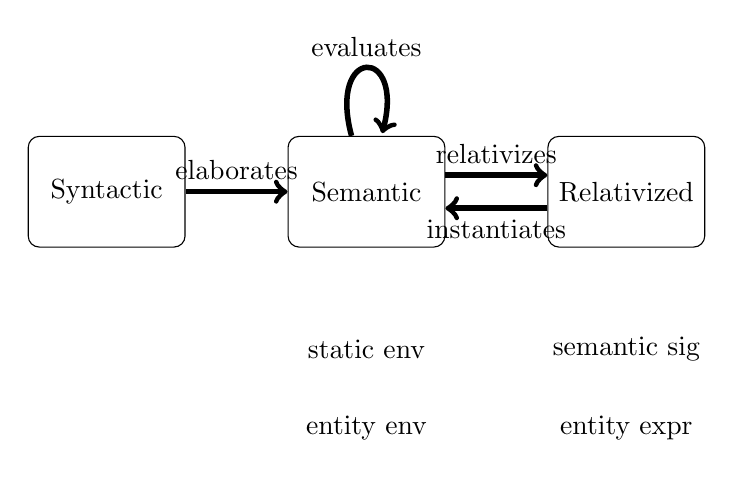
\begin{tikzpicture}[node distance= 3.3cm,auto]
\tikzstyle{block} = [rectangle, draw,  
    text width=5em, text centered, rounded corners, minimum height=4em]
\tikzstyle{arr} = [line width=2pt,->]
	\node[block] (sy) {Syntactic};
	\node[block, right of=sy] (se) {Semantic};
	\node[block, right of=se] (re) {Relativized};

	\node[node distance=2cm,below of=se] (statenv) {static env};
	\node[node distance=1cm,,below of=statenv] {entity env};
	\node[node distance=2cm,below of=re] (semsig) {semantic sig};
	\node[node distance=1cm,below of=semsig]  {entity expr};
		
	\path[arr] (sy) edge node {elaborates} (se);
	\path[arr] ([yshift=-5mm]se.north east) edge node {relativizes} ([yshift=-5mm]re.north west);
	\path[arr] (se) edge [loop above] node {evaluates} (se);
	\path[arr] ([yshift=5mm]re.south west) edge node {instantiates} ([yshift=5mm]se.south east);
	

\end{tikzpicture}
\end{center}
\caption{Life-cycle of a tycon}
\label{fig:lifecycle}
\end{figure}
%% DBM: I modified fig:semtypesystem to include entpaths as possible
%% tycons, which merges semantic tycons and relativized tycons.  The
%% relativized tycons then just become semantic tycons in which at least
%% one entpath occurs.  This simplifies things in the sense that we don't
%% need another set of tycon/type expression metavariables, but does
%% it add complications elsewhere?

\subsection{Relativized Type System}\label{sec:relativized-type-sys}
The relativized type system ($\mathbb{C}^s, \mathbb{C}^\lambda,$ and
$\mathbb{T}$) replaces all occurrences of atomic tycons with entity
paths.
%% DBM: not _all_ tycons -- only volatile ones.  Absolute, nonvolatile
%% tycons can remain in place.  Since relativized types have both
%% regular and entpath tycons, an absolute type is just an extreme
%% case of a relativized type where there are 0 entpath tycons.
%% In other words, the semantic tycons should be viewed as a subset
%% of the relativized tycons.
The purpose of relativization and this type system is described
in section~\ref{sec:volatile}. Three classes of tycons have been
introduced: syntactic, semantic, and relativized. The semantics
progressively translates syntactic tycons to the latter two. The
module system only evaluates semantic tycons. Such tycons exist in the
static and entity environments. In contrast, relativized tycons are
never reduced directly. Instead, they must be instantiated into a
semantic tycon for reduction to take place as in
fig.~\ref{fig:lifecycle}. Relativized tycons exist in semantic
signatures and static environment by way of embedded semantic
signatures.

%% DBM: too routine to mention, and redundant if we view them as a
%% subset of semantic types/tycons
% Relativized monotypes, tycons, and types must also be well-kinded as
% defined in Fig.~\ref{fig:relativized-wellkinding}. The main difference
% between this well-kinding judgment and the other well-kinding
% judgments is that rule~\ref{eq:r-k-app} uses the entity environment to
% obtain a well-kinded {\bf semantic} tycon. The rest of the semantics
% is standard. 

%% DBM: we never have to determine equivalence of uninterpreted 
%% relativized types.  For the purpose of type checking, we will
%% always be working with fully interpreted (absolute) types.
The rules in Figs.~\ref{fig:mt-tyc-equiv} and~\ref{fig:typeequiv}
define monotype and tycon equivalences and type expressions
equivalences respectively.  The module system semantics will require a
notion of relativized monotype equivalence and relativized tycon
equivalence, which are given by rules~\ref{eq:mtequiv}
and~\ref{eq:tcequiv} respectively.  Monotypes and tycons are
equivalent under the interpretation of an entity environment when they
evaluate to equivalent normal form semantic tycons modulo
$\alpha$-renaming. Rules~\ref{eq:teequiv-typ}
and~\ref{eq:teequiv-forall} describe equivalence for type expressions.

\subsection{Role of Relativization}
Relativization plays in a role in signature extraction (discussed in sec.~\ref{sec:sigextract}):
\begin{enumerate}
\item Value bindings in the static environment must be relativized. 
\item Definitional type binding in the static environment must be relativized in the inferred signature. 
\end{enumerate}
        
\begin{lstlisting}
sig
  structure M : sig type t end
  type u = M.t 
end
\end{lstlisting}

\noindent The type definition for u must be relativized because it refers not to a concrete type, but a type defined relative to a matching structure's realization.

Consider the following example:
\begin{lstlisting}
structure A =
struct
  structure B = struct datatype u end
  functor F(X:sig type t end) = 
    struct val a : X.t * B.u = ... end : sig val a : X.t * B.u end
end
\end{lstlisting}

The following are the semantic signatures for the example:
\[B \mapsto (\rho_B, \{u \mapsto (\rho_u, 0)\})\]
\[X \mapsto (\rho_X, \{t \mapsto (\rho_t, 0)\})\]
In the type for a, the tycon for X.t must be relativized to $\rho_X\rho_t$ and for B.u to $\rho_B\rho_u$. 

When inferring the signature from the body of F, we have the formal tycon X.t in the static environment. When inferring the signature from F's body, there are two static environments, the static environment produced by elaborating F's body and the contextual static environment when entering into the body. 

Static environment for F's body: $[a \mapsto \tau_t^0 * \tau_u^0 ]$ \\
Static environment for the context: $[B \mapsto (\rho_B, \{u \mapsto (\rho_u, \tau_u^0)\}, R_B)]$\\
                 $[X \mapsto (\rho_X, {t \mapsto (\rho_t, \tau_t^0)}, R_X)]$

$R_B$ and $R_X$ are the structure entities for $B$ and $X$ respectively. 


\begin{lstlisting}
structure A =
struct [$\rho_A$]
  structure B = struct [$\rho_B$] datatype t [$\rho_t$] = K end
  functor F(X [$\rho_X$]:sig type u [$\rho_u$] val a : u end) =
  struct 
    val b : X.u * B.t = (X.a, B.K)
  end : sig val b : X.u * B.t end
end
\end{lstlisting}

The relativized tycon, an entity path, can be computed from the static environment at the point of elaboration. For example, when the elaborator reaches the body of the above functor, the static environment is the following:

$[B\mapsto (\rho_B, \langle \{t \mapsto (\rho_t, 0)\}, \emptyset_{ee}\rangle)][X\mapsto (\rho_X,\langle\{u\mapsto(\rho_u,0), a\mapsto [\rho_u]\},\emptyset_{ee}\rangle)]$

The tycon for \lstinline{X.u} can be relativized by building an entity path, \emph{i.e.}, $\rho_X\rho_u$, by traversing the static environment. 

When elaborating the specified type of \lstinline{a} in the functor parameter signature, the reference to the formal tycon \lstinline{u} is relativized to an entity path $\rho_u$. 

After instantiation of the parameter signature during functor elaboration (sec.~\ref{sec:modelab}),  the elaborator must derive the canonical entity path for any newly generated tycons, structures, and functors, which will correspond to an entity variable in the parameter signature. The elaborator uses the canonical entity path when elaborating the functor result signature and functor body. 

This after-the-fact entity to entity path mapping is also needed for structure bindings to create the mappings for coerced entities produced during signature matching. Unlike in the functor case, mappings for the entities in the structure binding and the structure entity itself must be in scope for the rest of the program. 

A policy of fully reducing a tycon before relativizing 
simplifies the process of relativization. Each primary
volatile tycon has a unique declaration site and thus a unique entry in the
entity environment from which the elaborator can derive the unique
entity path leading to that tycon. 

$\Upsilon$ is a sequence of bindings of entity variables to
entities. A binding $[\rho\mapsto\upsilon]$ in $\Upsilon$
\emph{precedes} another binding $[\rho'\mapsto\upsilon']$ if it comes
earlier in the sequence. Note that since entity environments are
hierarchical, one binding can precede another even if they are not in
the same level in the hierarchy.  Let ($\sqsubseteq_{ee}, \Upsilon$) be the total ordering of
the entity paths in $\Upsilon$. Let $\vec{\rho}_1 \sqsubseteq_{ee}
\vec{\rho}_2$ only if the entity environment binding denoted by
$\vec{\rho}_1$ precedes the binding for $\vec{\rho}_2$. Let
$\inv(\Upsilon, \tau^n)$ denote the least entity path $\vec{\rho}$ with respect to
$\sqsubseteq_{ee}$ such that $\Upsilon(\vec{\rho}) = \tau^n$. 

The definition of relativization
uses an operation of the entity environment $\inv$ to
calculate the entity path. Although $\Upsilon$ technically does not
admit an inverse because multiple entity paths may map to the same
atomic tycon, this operation is intuitively similar to an inverse of $\Upsilon$ lookup. 

\begin{definition}
$\inv(\Upsilon,\tau^n)$ is defined to be the entity path associated
with the first occurrence (\ie, least binding according to $\sqsubseteq_{ee}$) of $\tau^n$ when treating the entity environment $\Upsilon$ as a sequence of bindings. 
\end{definition}

\begin{example}
Let $\Upsilon=[\rho_0\mapsto [\rho_1\mapsto \tau^0_1]][\rho_2\mapsto \tau^0_1]$. $\inv(\Upsilon,\tau^0_1) = \rho_0\rho_1$. 
\end{example}

\subsection{Semantics}

Fig.~\ref{fig:eprelativize} formally defines the relativization of
syntactic monotypes, tycons, and type expressions. 
The relativization judgments require an
entity environment $\Upsilon$ to interpret atomic tycons associated
with those symbolic paths.

Relativization is used in signature expression elaboration of where type~(\ref{eq:wheretype}), type definition spec elaboration~(rule~\ref{eq:typedefspec}), val spec elaboration~(rule~\ref{eq:valspec}), and signature extraction (rules~\ref{eq:extraval},\ref{eq:extratypedef}). 

\begin{definition}[Well-formedness of entity environments]\label{def:wellformedentenvs}
\begin{enumerate}
\item If $\Gamma,\emptyset_{knds} \vdash \vec{\rho} :: \Omega^n \to \Omega$, then $\Upsilon(\vec{\rho}) = \tau^n$ or $\Upsilon(\vec{\rho}) = \mathfrak{C}^\lambda$ such that $|\mathfrak{C}^\lambda| = n$. 

\item If $\vec{\rho}$ is a functor in $\Gamma$, then $\Upsilon(\vec{\rho}) = \psi$. 

\item If $\vec{\rho}$ is a structure in $\Gamma$, then $\Upsilon(\vec{\rho}) = R$. 
\end{enumerate}
\end{definition}

\section{Elaboration Semantics}

In a first-order module system, functor application can propagate types in the parameter to the functor result. True higher-order semantics is useful for compilation of efficient module code \cite{shao98}. More importantly, type propagation is necessary to make some sound programs typecheck. THO semantics also reflects the dependent type structure of functors. Types in the functor parameter may also be generative, as in the case of datatypes and types in opaquely ascribed substructures. These generative types have to be faithfully propagated during functor application. Functors complicate type propagation because types in the functor result may be computed from multiple sources. As in the first-order case, types may be locally defined in the result or propagated from the parameter. Applications of formal functors (\ie, functors in the functor parameter) in the functor result should also propagates types. Collectively, generation of fresh instances of generative types and formal functor applications are called \emph{functor actions}, which must be performed during elaboration of functor application to maximize type propagation.    
 
As in other accounts of module system designs, I present the THO module system as an elaboration semantics. The syntactic module language is elaborated to a semantic representation. Unlike prior accounts, this semantics will use an entity calculus that captures the functor actions in a program. The entity calculus is a third level of representation distinct from the syntactic and semantic representations. It assumes that each type is given a unique name, an entity variable. Unlike other internal languages, the entity calculus only plays a role in elaboration. Entity calculus terms are translated to IL types by the time code reaches the optimization stages of a compiler. 
      
Elaboration accomplishes the following:
\begin{enumerate}   
	\item Produces a static environment mapping variables to static descriptions of values, types, structures, functors, and signatures
	\item Produces a typed abstract syntax
	\item Produces entity expressions used in representing functor actions
	\item Typechecks the program
\end{enumerate}

For simplicity, the discussion of (2) will be postponed to chapter~\ref{ch:translation}. Fig.~\ref{fig:overview} shows the major components of the elaboration process and how they are related. 

\begin{figure}
\begin{center}
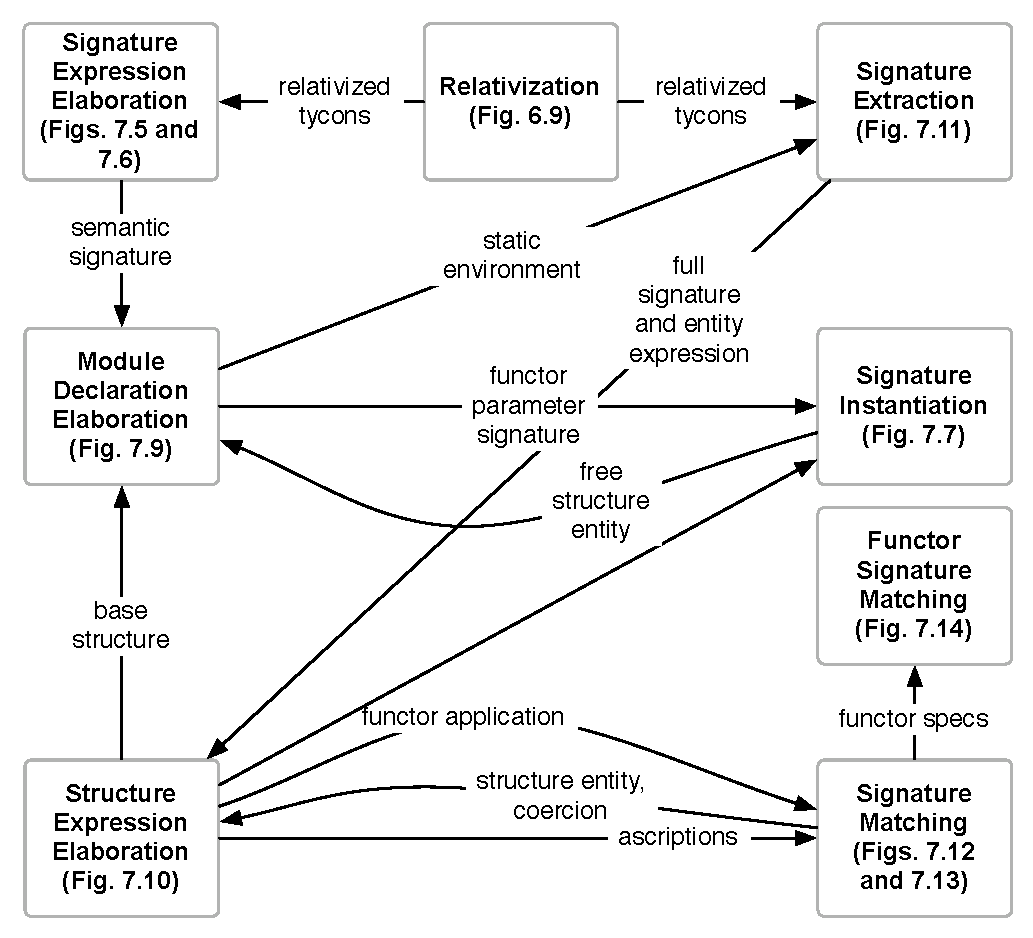
\includegraphics[scale=0.4]{../dissertation/figs/overview}
\end{center}
\caption{Map of elaboration processes}
\label{fig:overview}
\end{figure}
 
% \section{Why Higher-Order Functors?}
% The Fox project at CMU demonstrated that functors are valuable for the design and organization of extensible software systems. Shao~\cite{shao:parameterizedsigsandho}  demonstrates that higher-order functors are necessary for precisely expressing the import signature of a module that refers to externally defined functors. This idea is motivated by the \emph{fully functorized style} originally espoused by Tofte. 


\section{Elaboration Representations}
Elaboration is mainly concerned with the construction of a static environment. Secondarily, the elaborator produces typed abstract syntax, an entity environment, and an entity expression. The static environment contains the visible static information in the elaborated program. The static information comes in the form of semantic representations of signatures and type information. 

\begin{lstlisting}
sig
   type t [$\rho_t$] 
   type u = int 
   structure M [$\rho_M$] : sig type s [$\rho_s$] end
end
\end{lstlisting}
 
The entity environment contains static information that may have been occulted by shadowing and the functor actions describing the production of new static information during functor application. Much of elaboration is concerned with constructing the correct entity environment and using them to interpret entity paths. 

\subsection{Semantic Objects}
A semantic signature is a sequence of signature elements, symbol to spec bindings. Signature elements can be volatile ($s^p$), definitional ($\mathbb{C}^\lambda$), or a value spec ($\mathbb{T}$). Note that all signature spec elements must be relativized. Nonvolatile elements including definitional tycons $\mathbb{C}^\lambda$ and value specs $\mathbb{T}$ need only specify their fixed static description. Volatile primary specs ($s^p$) such open ones $arity$, structures $\Sigma$, and functors $\Sigma^f$ may be instantiated by signature matching and thus must have a corresponding binding in the entity environment indexed by entity variables. A \emph{full signature M} gives a full semantic description of a structure. It is comprised of a semantic signature $\Sigma$ and a structure entity $R$ that interprets all the open specifications in $\Sigma$. 

A semantic functor signature $\Sigma^f$ binds an entity variable for the functor parameter $\rho$ in the functor result signature. A full functor signature $F$ is comprised a semantic functor signature $\Sigma^f$ and a functor entity $\psi$ that when evaluated will interpret all the open specifications in the functor result signature. 

$\gamma$ is a static binding, to which the static environment $\Gamma$ maps identifiers. For value identifiers, the static description is a semantic type expression $\mathfrak{T}$. For tycon definitions, the static description is $\mathfrak{C}^\lambda$. There is no static binding for open tycon because all tycons are either defined or instantiated in the static environment.  For signature and functor signature identifiers, the static descriptions are semantic signatures ($\Sigma$) and semantic functor signature ($\Sigma^f$). For structure and functor identifiers, the static descriptions are full signatures and full functor signatures respectively. Some static binding (namely for structures and functors) consist of the full signature or full functor signature coupled with the entity variable for that structure or functor. The entity variable is used to construct entity paths during signature extraction and elaboration. 

Tycons in signatures and in static environments differ in that tycons
in the former will have been relativized during signature elaboration
or extraction. Unlike static environments that may be extended
throughout the elaboration process, signatures do not change. Hence to
ensure that volatile tycons in signatures have an appropriate
interpretation, they must be relativized with respect to the entity
environment. 

\begin{figure}
\begin{center}
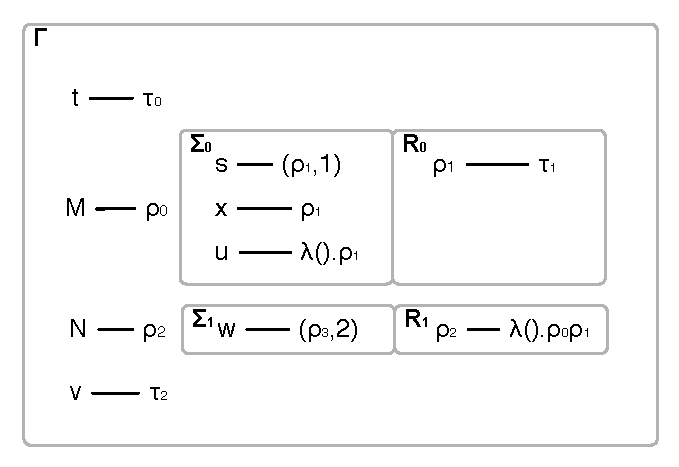
\includegraphics[scale=0.5]{../dissertation/figs/fig-staticenv-sigs}
\end{center}
\caption{Schematic of static environment}
\label{fig:staticenv-sigs}
\end{figure}

In Fig.~\ref{fig:staticenv-sigs}, the static environment depicted
exhibits the heterogeneous form of the definition. The first layer
contains semantic tycons, those types directly bound by the static
environment. The second layer consist of the tycons $s, u,$ and $w$ bound in semantic
signatures $\Sigma_0$ and $\Sigma_1$ embedded inside of the static
environment. These semantic signatures contain relativized tycons. The
full signature for structures also include the structure entity
expressions $R_0$ and $R_1$ which define the instantiation of the open
tycons in the corresponding semantic signature.  


\section{Notation}\label{sec:elabnotation}

If $p$ is a symbolic path and $\Sigma$ is a semantic signature, then $p\in\Sigma$ means that following $p$ in $\Sigma$ reaches a spec. If $p$ is a singleton, then $\Sigma$ must contain a binding $p\mapsto spec$. Otherwise, if $p$ is nonsingleton, then $p=xp'$ such that $x$ is a symbol and $p'$ is a symbolic path such that $\Sigma$ contains a binding $x\mapsto (\rho,\Sigma')$ and $p'\in\Sigma$. 

$\Sigma(p)$ is the spec reached by following $p$ in $\Sigma$. The notation $\EP(\Sigma,p)$ denotes the entity path associated with the signature spec referred to by symbolic path $p$. The entity path is comprised of the entity variables on the path to the element. For example, if the signature is $\Sigma = [A\mapsto(\rho_A,[B\mapsto (\rho_B, [t \mapsto (\rho_t, 0)])])]$, then $\Sigma_{ep}(A.B.t) = \rho_A\rho_B\rho_t$. The same notation is extended to static environments. 

Static environment lookup is expressed as $\Gamma(p)$ where $p$ is the symbolic path to the static binding. If $p$ is a singleton, then the static environment lookup would simply return the corresponding static binding. As will be demonstrated below, static environment lookup sometimes requires an entity environment lookup. This is the case when the component being looked up is a definitional tycon in a nonsingleton path. Depending on what kind of entity $p$ refers to, the lookup is handled differently:
\begin{description}
\item[tycon]~
\begin{description}
\item[singleton path $p=x$] The semantic tycon is $\Gamma(x)$.
\item[nonsingleton $p=q.x$] $\Gamma(q)$ produces a full signature ($\Sigma_q,R_q$). Let $\Upsilon_q = \Uclo\Uloc$ where $R_q = \langle \Uloc, \Uclo\rangle$. 

If $\Sigma_q(x) = (\rho_x,n)$, then $\Gamma(p) = \Upsilon_q(\rho_x)$. 

If $\Sigma_q(x) = \mathbb{C}^\lambda$, then $\Gamma(p) = $ the interpretation of $\mathbb{C}^\lambda$ under $\Upsilon_q$. 

Note that all tycons are interpreted using the structure entity closest to the occurrence. 
\end{description}
\item[full signature or a full functor signature] $\Gamma(p)$ denotes a pair $(\vec{\rho}, M)$ such that $\vec{\rho}$ is the entity path to the structure static binding and $M$ is the full signature of that structure. For example, for $\Gamma=[A\mapsto(\rho_A,([B\mapsto(\rho_B, \Sigma_B)], R_A))]$, $\Gamma(A.B) = (\rho_A\rho_B, (\Sigma_B,R_A(\rho_A\rho_B)))$. 
\end{description}

\section{Elaboration Modes}
During elaboration, entity expressions are both produced and consumed to aid in typechecking. Elaboration occurs in two simultaneous modes: the \emph{direct mode} and the \emph{entity compilation mode}. Direct mode consists of core language type checking, direct construction of entity expressions (such as tycon declaration elaboration and signature instantiation), and evaluation of entity expressions from the static information uncovered during elaboration. The main results of this mode are a static environment mapping symbolic names to static descriptions and an entity environment mapping entity variables to entities. The evaluation of entity expressions may produce new entities which added to static and entity environments. The entity compilation mode compiles functor actions into entity expressions.   

Elaboration is entirely a compile-time process. The entity language is distinct from core and module languages. The language is parallel to the semantic representation and the syntactic language. Elaboration translates core and module languages to typed abstract syntax and entity expressions. The part of elaboration that produces entity expressions and declaration is called \emph{static entity compilation}. Because the entity language is intended to describe functor actions, which are not encoded in the typed abstract syntax, the two are complementary. When the elaborator reaches a functor application in the source, the corresponding application entity expression must be evaluated to produce the static information for the result. Entity expression evaluation yields structure entities. 
   
\section{Entity Compilation Mode}
Besides the direct elaboration mode for the evaluation of entity expressions, described in chapter~\ref{ch:entitycalc}, the elaborator must have an entity compilation mode that produces the entity expressions and semantic representations of the modules from the syntax. The process of the compilation mode is the bulk of the elaboration semantics. Entity expressions for both structures and functors are compiled from the raw implicitly typed abstract syntax trees and the contextual environments used during elaboration. The compilation mode elaboration is the subject of the remainder of this chapter. 

The compilation mode elaboration compiles abstract
syntax trees to entity expressions. All of elaboration takes place
under a static environment $\Gamma$. Recall that semantic
signatures pair all static primary components with entity variables
and replace all occurrences of such primaries with a canonical entity path to the corresponding static entity in the entity environment, which is calculated by relativization. Values are classified by their type. Structures are described by their full signature consisting of a structure entity and a signature. A functor static description is a full functor signature, comprised of a functor entity expression (\ie, a $\lambda$-expression) and a functor signature. The main elaboration judgments are the following:\\
 
\begin{tabular}{ll}
        $\Gamma,\Upsilon,\Sigma\vdash C^s \Rightarrow_{mt} \mathfrak{C}^s$ & monotype elaboration\\
        $\Gamma,\Upsilon,\Sigma\vdash C^\lambda \Rightarrow_{tyc} \mathfrak{C}^\lambda$ & tycon elaboration\\
        $\Gamma,\Upsilon,\Sigma\vdash T \Rightarrow_{te} \mathfrak{T}$ & type elaboration\\
\end{tabular}\\

The above judgments produce semantic monotypes/tycons/type expressions from syntactic ones. Tycon elaboration's sole role is during elaboration of tycon declarations (rule~\ref{eq:typedefdecl}). 

\begin{tabular}{ll}       
        $\Upsilon\vdash \mathfrak{C}^s \searrow^{mt} \mathbb{C}^s$ & monotype relativization\\
        $\Upsilon,\Sigma\vdash \mathfrak{C}^\lambda \searrow^{tyc} \mathbb{C}^\lambda$ & tycon relativization\\
        $\Upsilon,\Sigma\vdash T \searrow^{te} \mathbb{T}$ & type expression relativization
\end{tabular}\\

The relativization judgment produce relativized tycons from syntactic ones. The entity environment $\Upsilon$ is used to relativize the nonlocally defined tycons. The signature $\Sigma$ is used to construct relativized entity paths for locally defined tycons. Signature extraction and elaboration rely on relativization. \\

\begin{tabular}{ll}      
$\Gamma,\Upsilon,\Sigma\vdash sigexp \Rightarrow_{sig} \Sigma'$ & signature elaboration\\
$\Gamma,\Upsilon,\Sigma\vdash fsgexp \Rightarrow_{fsg} \Sigma^f$ & functor sig elaboration\\
        $\Uclo,\Uloc\vdash \Sigma \uparrow \Uloc$ & signature instantiation\\
        $\Gamma,\Upsilon\vdash d^m \Rightarrow_{decl} (\eta,\Gamma',\Upsilon')$ & module decl elaboration\\
        $\Gamma,\Upsilon\vdash strexp \Rightarrow_{str} (M, \varphi)$ & structure expr elaboration\\
        $\Upsilon\vdash\Gamma\hookrightarrow \Sigma$ & signature extraction\\
        $\Upsilon\vdash(M,\varphi):\Sigma\Rightarrow_{m} (M_c,\varphi_c)$ & signature matching\\
        $\Upsilon\vdash F \preceq \Sigma^f \Rightarrow_{fsgm} (\psi_c, \theta_c)$ & functor signature matching
\end{tabular}

\section{Type Constructors}
The syntactic type language is a subset of the semantic tycon language. Before proceeding, the elaborator must first elaborate the syntactic types to semantic tycons. The elaboration is simply a syntax-directed recursive translation. 

The syntactic type language elaborates to the semantic type language. Elaboration interprets the symbolic paths in tycon application $p(\vv{C^s})$ and evaluates the application by standard $\beta$-reduction. Note that tycon elaboration $\Rightarrow_{tyc }$ elaborates and therefore reduces under $\lambda$-abstraction. This ensures that tycon definitions are fully reduced. Because $\lambda$s cannot be nested, this reduction is well-defined and normalizing. The normal form is defined as $\mathfrak{C}^{nf}$ in fig.~\ref{fig:semtypesystem}. 

Note that the tycon may be occuring inside a signature spec, in which case it may refer to entity paths for preceding specs. 

\begin{lstlisting}
sig 
  type t
  type u = t
end
\end{lstlisting}

During the elaboration of the above, t will be given an entity variable. When elaborating the occurrence of tycon t in the definition of u, t is not the static environment. It can only be found in the partial semantic signature produced by elaborating the open spec for t. Signature specs may contain relativized tycons, entity paths,
referencing entities declared earlier in the same semantic signature. These preceding signature specs (forming a semantic signature $\Sigma$ itself)
help construct an entity path for symbolic paths not defined in the
static environment. Rule~\ref{eq:tycapp} uses $\entpath$ to calculate the entity path using static and entity environments. In order
to fully relativize such a symbolic path, the $\entpath$ metafunction
needs to first lookup the symbolic path in the preceding signature
specs $\Sigma$, which contains all the preceding specs in the current signature and only if that fails does it look up in the static environment.  


The type elaboration judgments preserve the well-kinding defined in chapter~\ref{ch:typesystem}.

\begin{lemma}[Monotype Elaboration Preserves Kinding]
If $\Gamma,\emptyset_{knds}\vdash C^s : \Omega$ and $\Gamma,\Upsilon\vdash C^s \Rightarrow_{mt} \mathfrak{C}^s$, then $\emptyset_{knds}\vdash \mathfrak{C}^s : \Omega$. 
\end{lemma}

\begin{lemma}[Tycon Elaboration Preserves Kinding]
If $\Gamma,\emptyset_{knds}\vdash C^\lambda : \Omega^n \Rightarrow
\Omega$ and $\Gamma,\Upsilon\vdash C^\lambda \Rightarrow_{tyc}
\mathfrak{C}^\lambda$, then $\emptyset_{knds}\vdash \mathfrak{C}^\lambda : \Omega^n \Rightarrow \Omega$.
\end{lemma}

\section{Signature Elaboration}
The role of signature elaboration is to relativize tycons, to reduce where type clauses to type definitions, and to decorate all specs corresponding to static entities with  entity variables. The elaboration judgment uses static and entity environment to interpret symbolic paths in tycon definitions. However, not all symbolic paths are bound in the static environment. For example, in the following signature, the type definition for u mentions tycon t which does not have a corresponding structure entity at this point, hence tycon t will not be in static and entity environment. 

\begin{lstlisting}
sig type t type u = t end
\end{lstlisting}

Rule~\ref{eq:specs} composes the result of elaborating the individual specs. Elaborating subsequent specs in the same signature will require a context (a signature) that includes all the previously elaborated specs $\Sigma$ and the newly elaborated spec $\Sigma'$.  

Signature spec elaboration produces entity variables for each static
component (\emph{i.e.}, open type specs, structure spec, and functor
spec) and puts them in the resultant semantic
signature. Rules~\ref{eq:typedefspec} and~\ref{eq:valspec} relativize
semantic tycons and type expressions respectively. 

In particular, the signature $\Sigma$ is needed when relativizing specs in a signature $\Sigma'$ that contain symbolic paths defined within the same $\Sigma$. Latter specs can contain symbolic paths declared in earlier specs within the same signature. Because the signature is not yet fully elaborated and does not correspond to any full signature, it is neither defined in the static environment nor the entity environment, each of which only mapping paths defined outside of the signature currently being elaborated. 


Rule~\ref{eq:fctspec} elaborate the formal parameter signature $sigexp_1$ and then the functor body signature $sigexp_2$ with the signature context extended with a spec corresponding to the formal parameter. 

Let $AT(\cdot)$ denote the set of all atomic tycons ($\tau^n$) in $\cdot$. 
The following lemma guarantees that all tycons are fully relativized by the relativization judgment. 

\begin{lemma}
If $AT(\Sigma) = \emptyset$, for all $\Sigma_i\in\Gamma.AT(\Sigma_i)=\emptyset$, and $\Gamma,\Upsilon,\Sigma\vdash sigexp \Rightarrow_{sig} \Sigma'$, then $AT(\Sigma') = \emptyset$. 
\end{lemma}

\section{Signature Instantiation}\label{sec:siginst}

Signature instantiation produces a free instantiation of a given
semantic signature, where free is in the context of both a closure and
a local entity environment. Instantiation produces an entity
environment that is local, meaning exclusive of closure entity
environment bindings (see rule~\ref{eq:inst-empty}). 

Most of the
judgments ignore the signature element. The elements that matter are
the those corresponding to static entities. Rule~\ref{eq:inst-open}
produces a fresh atomic tycon $\tau^n$ of the appropriate arity
$n$. The tycon must be fresh in both closure and local entity
environments. Subsequent signature elements must be instantiated in
the context of the local entity environment extended with the binding
to the new tycon $[\rho\mapsto\tau^n]$. This new binding serves two
roles. First, it ensures that $\tau^n$ is not reused when
instantiating the rest of the signature elements. Second, the new
binding may be included as part of the closure entity environment when
instantiating a structure and functor specs.  

Rule~\ref{eq:inst-str} instantiates a structure spec by recursively
instantiating its semantic signature. The structure's semantic signature may mention
either entities in $\Uclo$ and $\Uloc$, that is,
preceding entities in the same signature. The resulting entity environment
is combined with a closure $\Uclo\Uloc$ to form a
structure entity. Rule~\ref{eq:inst-fct} instantiates a functor spec
by producing a functor entity contains a formal functor functor entity
expression $\lambda\rho_x.\Sigma_r$ and a closure entity
environment. 

\begin{lemma}[Signature Instantiation Terminates]
$\Upsilon\vdash \Sigma \uparrow \Upsilon'$ terminates.
\end{lemma}

% \section{Top Level Declaration Elaborations}

% Elaboration of top level declaration is
% straightforward. The semantics is given in Fig.~\ref{fig:toplevel}. Rule~\ref{eq:sigdec} elaborates a signature
% expression and extends the static environment with a binding of the
% signature name to the semantic signature. Rule~\ref{eq:topmoddec}
% elaborates module declarations using the $\Gamma,\Upsilon\vdash d^m
% \Rightarrow_{decl} (\eta,\Gamma',\Upsilon')$ judgment. The judgment
% can safely discard the entity declarations from the module
% declarations because top level declarations will not be wrapped in a
% functor and therefore lead to functor actions. 

\section{Signature Extraction}\label{sec:sigextract}

Fig.~\ref{fig:extractsig} gives the rules for signature extraction, the process of synthesizing a semantic signature for a structure given only the static environment produced by elaborating that structure and an entity environment. Because the signature must contain only relativized type expressions and tycons, rules~\ref{eq:extraval} and~\ref{eq:extratypedef} must relativize the semantic type expression and tycon in the static environment. Rule~\ref{eq:extraatomictyc} produces a spec from an atomic tycon binding, which specifies the arity $n$ of the tycon. The rule looks up the atomic tycon in the ``inverse'' of $\Upsilon$. This rule assumes that $\Upsilon$ and $\Gamma$ are synchronized. In particular, since $t$ is a local name in the static environment (\emph{i.e.}, its binding is not nested inside some signature in $\Gamma$), $\tau^n$ should also be local in $\Upsilon$ and therefore have a singleton entity path. 
 
\begin{lemma}[Synchronization of Static and Entity Environments]
If $\Gamma,\Upsilon \vdash d^m \Rightarrow_{decl} (\eta, \Gamma', \Upsilon')$ and $EV(\Gamma)\subseteq dom(\Upsilon)$, then $EV(\Gamma')\subseteq dom(\Upsilon')$. 
\end{lemma}

For full signatures and full functor signatures, signature extraction is simple. Rules~\ref{eq:extrastr} and~\ref{eq:extrafct} forms structure and functor specs by projecting out the entity variable and semantic signature (or semantic functor signature) from the static environment mapping for the structure and functor respectively. 

\section{Signature Matching}\label{sec:sigmatch}
Signature matching plays three principal roles during elaboration. It
coerces functor arguments to the form dictated by the functor
parameter signature in
rule~\ref{eq:strapp}. Rules~\ref{eq:transascription}
and~\ref{eq:opaqueascription} use signature matching to constrain the
full signature of the structure for transparent and opaque ascription
respectively. Figs.~\ref{fig:sigmatch} and~\ref{fig:specmtch} describe 
the signature matching judgment and its subsidiary judgment respectively. The main judgment for signature matching $\Upsilon\vdash(M,\varphi):\Sigma\Rightarrow_{match} (R_c,\varphi_c)$ forms the \emph{coercion structure entity expression} $\varphi_c$ which binds the uncoerced, original entity expression to a fresh entity variable $\rho_u$ for use by the coercion entity declarations $\eta$. In general, $\eta$ may alias components of $\varphi$ as is in the case in rule~\ref{eq:coerceopen}.  The coercion structure entity expression needs both $\varphi$ and $\eta$ because the elaborator needs to evaluate $\varphi$ at least for its functor actions and $\eta$ are the actual exported entity variables. The entity environment for signature matching is a composite of the context $\Upsilon$, actual structure local environment $\Upsilon_a$, and actual structure closure environment $\Uclo$. All three are necessary because $\Upsilon$ closes the spec signature $\Sigma_s$, $\Upsilon_a$ the actual $\Sigma_a$, and $\Uclo$ the local environment $\Upsilon_a$. 

A subsidiary judgment $\Upsilon,\Sigma_a,\rho_u\vdash \Sigma_s \Rightarrow_{coerce} (\Upsilon', \eta)$ matches actual structure components to individual specs. The actual structure signature $\Sigma_a$ is used to match against each spec. The entity variable $\rho_u$ provides access to the uncoerced structure entity expression in case the elaborator needs to alias components. The judgment will produce both a semantic signature and a local entity environment, used by the match judgment to produce a coerced full signature. 

Rule~\ref{eq:coerceempty} matches against an empty spec signature, in
which case the coercion signature, entity environment, and entity
declarations are empty. Rule~\ref{eq:coerceval} matches value specs
only when the value's type expressions are equivalent when interpreted
under the entity environment. For open tycon specs, there are two
cases. Rule~\ref{eq:coerceopen} matches an open tycon spec against an
open tycon spec in actual. In that case, the rule will use the
structure entity for the actual and an alias to the entity path for
the actual $\rho_u\rho_a$ for the entity
declaration. Rule~\ref{eq:coerceopenwithdef} matches an open tycon
spec against a definitional tycon spec in the actual. The arities of
the definitional tycon and the open tycon spec must match
up. Rule~\ref{eq:coercedefdef} matches a definitional tycon spec in
the spec signature to a definitional tycon spec in the actual. Again,
this match requires the equivalence of the spec and actual
definitional tycons interpreted under the entity
environment. Rule~\ref{eq:coercedefwithdt} matches a definition tycon
spec in the spec signature to an open tycon in the actual, which should be consistent with the tycon in entity environment $\Upsilon(\rho)$. Rules~\ref{eq:coercestr} and \ref{eq:coercefct} match structure and functor specs respectively. Being specs for entities, these rules must produce a new entity environment binding and entity declaration. Rule~\ref{eq:coercestr} forms the bindings using the full signature and structure entity expression from performing signature matching on the signature in the structure spec. The full signature the rule will match against is formed by the spec signature $\Sigma_x$ and the corresponding structure entity $\Upsilon(\rho_x)$. Rule~\ref{eq:coercefct} works similarly. 

The relationship between the resultant structure entity, the spec
signature, and actual signature is precise:

\begin{lemma}
If $\Upsilon \vdash ((\Sigma_a,R_a),\varphi) : \Sigma_s \Rightarrow_{match} (R_c,
\varphi_c)$, then for all $[x\mapsto s]\in\Sigma_s$, $[x\mapsto
s']\in\Sigma_a$ such that $R_c(s)=R_a(s')$.
\end{lemma}

An important property is that the structure entity expression
constructed by signature matching should evaluate to the coerced
entity environment up to isomorphism. The role of the structure entity
expression is to evaluate to an entity environment that instantiates
the spec signature to an actual argument structure in the current
entity environment.  

\begin{lemma}
If $\Upsilon \vdash ((\Sigma_a,R_a),\varphi) : \Sigma_s
\Rightarrow_{match} (R_c,\varphi_c)$, then $\Upsilon\vdash \varphi_c
\Downarrow_{str} R'$ such that $R_c$ is isomorphic to $R'$. 
\end{lemma}

\section{Functor Signature Matching}
Fig.~\ref{fig:fsgmtch} defines the functor signature matching judgment
$\Rightarrow_{fsgmtch}$ which is composed of a two rules,
rule~\ref{eq:fsgmtch-real} and~\ref{eq:fsgmtch-formal}. Both rules calculate a coerced functor entity
$\psi_c$ and functor entity expression $\theta_c$. To match the
functor spec, the functor spec's parameter signature $\Sigma_{spar}$
is matched against a full signature formed by the argument 
signature $\Sigma_{apar}$ and the instantiation of $\Sigma_{apar}$
plus a structure entity expression for the
argument. Rule~\ref{eq:fsgmtch-real} uses the structure entity
expression $\varphi$ for the a standard functor entity expression
$\lambda\rho.\varphi$. Rule~\ref{eq:fsgmtch-formal} only has a formal
functor entity expression $\lambda\rho.\Sigma$, 
The functor spec's result signature $\Sigma_{sres}$ is then
instantiated and that instantiation is used to form a full signature
for the functor result in order to match against the actual functor
spec's result signature $\Sigma_{ares}$. The resultant structure
entity expression can be used to form the final coerced $\psi_c$ and
$\theta_c$.  

\section{Module Elaboration}\label{sec:modelab}

The module elaboration judgment calls for a static environment and an entity environment as its context. The static environment serves to elaborate tycons and structures, by looking up symbolic paths. The entity environment plays a role in signature elaboration and instantiation of functor parameters. 

Fig.~\ref{fig:elabmod} gives the rules for elaborating module declarations. The judgment computes an entity declaration, a static environment, and an entity environment for the module declarations. The two environments will only contain bindings representing the information in the module declarations and not the closure. Each module declaration elaboration rule calculates a semantic representation of the declaration value (\emph{i.e.}, type expressions, (definitional) tycons, atomic tycons, full signatures, and full functor signatures) and binds that representation in the static environment (and the entity environment if the entity in question is primary). 

Rules~\ref{eq:valdecl} and~\ref{eq:typedefdecl} elaborate values to a
semantic type expression and syntactic tycon to semantic tycon
respectively. Rule~\ref{eq:valdecl} assumes a core expression elaboration (typechecking) judgment of the form $\Gamma\vdash e \Rightarrow_{core} \mathfrak{T}$, which is standard. Neither of these produce any entity declarations and
entity environment because they do not contain static
entities. Rule~\ref{eq:dtdecl} generates a fresh atomic tycon $\tau^n$
for a datatype. This atomic tycon is bound in both the static and
entity environments. The elaborator further produces an entity
declaration $\rho_t =_{tyc} \newx(n)$ that records the functor action
attributed to the datatype declaration. The entity declaration is
reserved for evaluation upon functor application of the possible
enclosing functor. When evaluated, it will produce another atomic
tycon distinct from the $\tau^n$ generated here. Rule~\ref{eq:strdecl}
elaborates the structure expression to a full signature and a
structure entity expression. Rule~\ref{eq:fctdecl} elaborates a
functor declaration via several steps: 
\begin{enumerate}
\item elaborate the functor parameter signature $\Sigma_x$
\item instantiate it $\Upsilon_x$
\item form a full signature using the result of the previous two steps $(\Sigma_x,R_x)$ where $R_x=\langle \Upsilon_x,\Upsilon\rangle$. 
\item elaborate the functor body using a static environment extended with this full signature and the entity environment extended with the structure entity 
\item form a full functor signature, a functor entity, and a functor entity expression using the structure entity expression from above
\end{enumerate}

Fig.~\ref{fig:strexpelab} elaborates a structure expression into a full signature and structure entity expression. Rule~\ref{eq:strpath} elaborates a structure path. The structure entity expression is an entity path, calculated by accumulating the entity variables in $\Gamma$ leading up to the element denoted by $p$. Rule~\ref{eq:basestr} must extract a semantic signature from the static environment produced by elaborating the base structure declarations. Rule~\ref{eq:strapp} elaborates a functor application in several steps:
\begin{enumerate}
\item looks up the entity path and full functor signature of the functor denoted by symbolic path $p$
\item elaborates the argument structure
\item coerces the argument structure and structure entity expression using the functor parameter signature by signature matching
\item forms the structure entity expression for the application 
\item evaluates the structure entity expression using the current entity environment
\end{enumerate}

Rule~\ref{eq:letexp} elaborates structure let expressions in the expected way. Rule~\ref{eq:transascription} elaborates transparent ascription by signature matching. Rule~\ref{eq:opaqueascription} elaborates opaque ascription by signature matching and then instantiating the spec signature to get fresh types for the open type specs. 

% Is the opaque ascription rule totally correct? It seems that using the spec signature and free instantion might be too much. 

An important invariant that must be maintained for module declaration elaboration is that all the atomic tycons in the static environment are also in the entity environment. This property guarantees that all atomic tycons can be relativized by the entity environment. 

\begin{lemma}
If $AT(\Gamma) \subseteq AT(\Upsilon)$ and $\Gamma,\Upsilon\vdash d^m \Rightarrow_{decl} (\eta,\Gamma',\Upsilon')$, then $AT(\Gamma') \subseteq AT(\Upsilon')$. 
\end{lemma}

The relationship between the semantic signature $\Sigma$ and structure
entity $R$ produced by elaboration is precisely related. $R$ is said
to \emph{interpret} $\Sigma$, which is defined as follows: 

\begin{definition}
$\Upsilon$ interprets $\Sigma$ if for all specs in $\Sigma$, one of the
following must be true:
\begin{enumerate}
\item If the spec is open$(\rho,n)$, then $\Upsilon(\rho)=\tau^n$
  or $\Upsilon(\rho)=\mathbb{C}^\lambda$ such that $\Upsilon\vdash
  \mathbb{C}^\lambda :: \Omega^n \to \Omega$. 
\item If the spec is a structure $(\rho,\Sigma')$, then $\Upsilon(\rho)=R'$ and $R'$ interprets $\Sigma'$. 
\item If the spec is a functor $(\rho,\Sigma^f)$, then 
  $\Upsilon(\rho)=\psi$. 
\end{enumerate}
\end{definition}

\begin{lemma}
If $\Upsilon$ interprets the extracted signature of $\Gamma$ and 
$\Gamma,\Upsilon\vdash strexp \Rightarrow_{str} ((\Sigma, R),
\varphi)$, then $R$ interprets $\Sigma$.
\end{lemma}

\section{Translation}

THO can be translated into an applied System
F$_\omega$ by decoupling the static and dynamic contents of modules.
Module systems that permit such decoupling are said to admit
\emph{phase separation} \cite{hmm:phasedist}. The elaboration
semantics given in the previous chapter is sufficient 
for typechecking. However, to support translation into F$_\omega$,
elaboration must annotate the abstract syntax with semantic objects. 

The translation rules assume an annotated module language that was
produced by an error-free elaboration. Since the program was
successfully elaborated, the semantics can make some assumptions about
the program, especially about what variables will or will not be accessed,
and thereby simplify the rules. %% Clarify or give example
The key information that must be retained are the entity variables,
the functor signature (particularly the semantic parameter signature),
and the full signature for arguments in functor applications. 

To translate structure expressions, we need both the semantic
signature and realization in the full signature for the
structure. Semantic signatures alone do not fully define the tycon
content of a structure, hence the realization is needed to look those
up. 

Translation of structure declarations and expressions is in the form
of the first two judgments in Fig.~\ref{fig:xlate-rules-summary}. The
third judgment constructs the kind information from the semantic
signatures corresponding to functor formal parameters. 
In the fourth judgment, the full
signature of a functor argument is needed to produce the type argument $c$
for the corresponding type application $e_\omega[c]$ because type
information lies in both the semantic signature and
realization. Similarly, the full functor signature is needed to
construct the F$_\omega$ tycon. 

\begin{figure}
\begin{tabular}{ll}
$d^m \leadsto_{dec} d$ & declarations\\
$strexp \leadsto_{exp} e_\omega$ & expressions\\
$\vdash \Sigma \leadsto_{knd} k$ & sem. signatures (kinds)\\
$\vdash M \leadsto_{tyc} c$ & full signatures\\
$\vdash F \leadsto_{fctspec} c$ & full functor signature\\
$\vdash \mathfrak{C}^{nf}
\leadsto_{type}^{nf} t$ & \\
$\Delta, \Upsilon\vdash \mathbb{C}^s
\leadsto_{type}^{tyc} t$ & \\
$\Upsilon\vdash\mathbb{T}\leadsto_{type}^{t}
t$ & \\
$\Upsilon\vdash \Sigma \leadsto_{type} lts$ & \\
\end{tabular}
\caption{Translation Rules}
\label{fig:xlate-rules-summary}
\end{figure}

% The notation $dom(d)$ here denotes the set of
% all the bound names,\ie, the $\rho$ in $\rho=e$. 

Rules~\ref{eq:transdec-str}
and~\ref{eq:transdec-fct} must produce declarations binding the entity
variable of the structure or functor instead of the syntactic
variable. % Is this necessary? Yes, structures and functors are static
          % entities but these rules only care about the dynamic
          % components for which there is no avoidance problem. 
The rule~\ref{eq:transdec-fct} will use the judgment $\vdash \Sigma
\leadsto_{sig} k$ defined in Fig.~\ref{fig:semsigtokinds} to extract
the kind information from the semantic signature for the functor
parameter. The type for the F$_\omega$ $\lambda$ abstraction is
calculated separately from the same semantic signature. 

Fig.~\ref{fig:transexp} gives the translation of the module
language expressions to F$_\omega$. Rule~\ref{eq:transexp-app} translates
structure applications. The functor being applied can be translated by
translating its entity path to the corresponding F$_\omega$ record
projection form. The actual argument structure expression is
translated to $e_\omega$, but the functor is expecting a parameter of
the form defined in full signature $M$. The associated coercion
structure expression $\letin{\rho_u=\varphi_u}{\llparenthesis \eta
  \rrparenthesis}$ can help produce coerced type and value
arguments. For the type argument, the rule translates the coercion entity
declaration to F$_\omega$ via the $\tycon$ function defined in
Fig.~\ref{fig:xlate-entdec}. For the value argument, reusing the
uncoerced expression by aliasing $\rho_{par} = \rho_u$ is sufficient
because the prior elaboration already guarantees that none of
components in $\rho_u$ that is not specified in the formal parameter
signature will be accessed. Furthermore, none of the variables are
being renamed. 

The F$_\omega$ kinds, tycons, and types for tycon content of structures, type
content of structures, and structures themselves are record kinds,
record tycons, and record types respectively. Each label-field pair is
a pair of an entity variable and the kind, tycon, and type of the
entity referred to by that entity variable. Let $lks$, $lcs$, and $lts$ be a sequence of record label-field for
kinds, tycons, and types respectively. The notation
$lks\uplus lks'$ appends two record kinds. The notation is extended in
the usual way to append tycons and types. No shadowing is expected
because all records field names will be entity variables. 

Fig.~\ref{fig:semsigtokinds} gives the rules for producing $F_\omega$
kinds from semantic signatures. Value specs and type definition specs
do not contribute to the kind (rules~\ref{eq:f-semsig-val} and~
\ref{eq:f-semsig-typedef}). Open tycon specs do
contribute. Rule~\ref{eq:f-semsig-opentype} produces the kind field
$\rho::\Omega^n \Rightarrow \Omega$ such that $n$ is the arity of the
open tycon spec. Rules~\ref{eq:f-semsig-str} and~\ref{eq:f-semsig-fct}
construct kinds for structure and functor specs from the semantic
signature and functor signature respectively. 

Fig.~\ref{fig:f-tycon-synthesis} defines the judgment that calculates
the tycons from the full signature of a structure. Again, value specs,
and type definition specs do not contribute to the tycon
(rules~\ref{eq:transspec-val} and~\ref{eq:transspec-typedef}).
Rule~\ref{eq:transspec-opentype} translates an open spec by looking up
the entity environment for the tycon entity associated with the open
tycon spec. The rule~\ref{eq:transspec-str} translates the structure
spec signature in the context of the entity environment calculated
from the structure entity
($\Upsilon(\rho)=\langle\Uloc,\Uclo\rangle=\Uclo\Uloc$).  To calculate
the tycon for a functor component, rule~\ref{eq:transspec-fct} must
supply rule~\ref{eq:trans-fctspec} the functor signature and entity
from looking up the entity environment. Rule~\ref{eq:trans-fctspec}
calculates the kind for the functor parameter using the parameter
signature and also the tycon for the functor body from the functor
body signature and closure entity environment. The judgment relies on
$\vdash \varphi \leadsto^{strexp}_{tyc} c$ which translates the
structure entity expression to the corresponding F$_\omega$ tycon
expression, which is the same because there is an embedding of the
structure entity expression language to the F$_\omega$ tycon
expression language. The above statement fully defines $\vdash \varphi
\leadsto^{strexp}_{tyc} c$.

Fig.~\ref{fig:fty-sig} gives the rules
for producing $F_\omega$ types from semantic signatures. These two
judgments decompose semantic signatures into kinds (for classifying
the static components) and types (for classifying the dynamic
components). Kind synthesis is used in rule~\ref{eq:fty-fct} to
produce the kind annotation for the polymorphic quantifier. 

Let the $\mathsf{env}(lts) = [\rho:t]$ where $\rho_i:t_i \in lts$ for
the purpose of fig.~\ref{fig:xlate-entdec}.

In the module system, subtyping in functor application may ``thin''
out an argument structure. To model this behavior in F$_\omega$, we
use a value-level coercion primitive $\coerce$. 
Fig.~\ref{fig:xlate-entdec} defines the function $\coerce$ that
coerces an F$_\omega$ expression $e_\omega$ to a record type $lts$. 
It thins out the value part by dropping components not
in the specified type. The resultant expression should have the target
type $\{lts\}\{c/\rho\}_{tyc}$ where $lts$ is parameterized by
$\rho$. The type-level coercion was already taken care of by
F$_\omega$ tycon synthesis. 

\begin{lemma}[Well-Typing of Coercions]
Let $E$ be a static environment (type and kind environment). 
If $E\vdash \rho_u : t_u$, $t_c\{c/\alpha\} = t_u$, and
$\coerce(\rho_u, c, t_c) = e_\omega$, then $E\vdash e_\omega : t_c\{c/\alpha\}$. 
\end{lemma}

\section{Soundness}

\begin{theorem}
If a closed structure expression $strexp$ elaborates to $(M, \_)$ and $strexp$
translates to $e_\omega$, then $\vdash e_\omega : t$ and $\vdash M \leadsto_{type} t$. 
\end{theorem}

The proof of the above lemma is sketched out in more detail in the
proof appendix. It relies on much of the same machinery as Shao's
proof~\cite{shao98}. The proof diverges in Shao's memoization of
pre-translated F$_\omega$ tycon and types in the functor
representation during elaboration of the functor. Furthermore, this
proof must deal with the coercive signature matching semantics which
is not present in Shao's main elaboration-translation semantics. 

\section{Type Generativity}

Shao's calculus and many of the related accounts of the module system
do not fully support the type generativity present in ML. Type
generativity stems from two constructs, opaque ascription and datatype
declarations. 

Seemingly benign examples that feature datatype declarations are not supported. 

\begin{lstlisting}
structure M = 
struct 
  datatype t
  val id : t -> t = fn x:t => x
end
\end{lstlisting}

\begin{lstlisting}
functor F() = 
struct
  datatype t
  val id : t -> t = fn x:t => x
end
\end{lstlisting}

Datatype declarations are an interesting case because unlike the rest
of the static content of a module, datatype declarations translate to
F$_\omega$ tycons that are not referentially transparent. Whereas all
other forms of F$_\omega$ tycons can be duplicated and be supplied as
arguments to type applications, the tycons from datatype declarations
cannot. This is because the identity of the tycon from a datatype must
be maintained. The tycon cannot be copied. Consequently, such a tycon
must be bound (by the special let tyc form) to a type variable that is
in the scope of all subsequent occurrences. It turns out that in
general, the expressions constructing these tycons are exactly the
entity expressions from the module system. The referentially
transparent static content such as type definitions can continue to be packaged together in a tycon record to which $\Lambda$ type abstractions can
be directly applied. 

Another difference between datatype declarations and type definitions
is what is translated into F$_\omega$. For datatype declarations, the
entity expression is translated. For type definitions, the full
signature is directly translated to an F$_\omega$ tycon. 

Translation decomposes functors into a tycon part and a value
part. The hat notation $\widehat{x}$ denotes the variable is a type
variable that refers to the type part of a structure or functor x. Let
$k$ represent $\Omega^0 \to \Omega$. 

\begin{lstlisting}
functor f(x:sig type s type t end) = 
struct datatype w type v = x.t end
\end{lstlisting}
\[\lettycline{\widehat{f}=\lambda \widehat{x}::\{s::k,t::k\}.\{w =
  \newx(0), v=\widehat{x}.t \}}
{\letin{f = \Lambda\widehat{x}::\{s::k, 
t:: k
    \}.\lambda x:\{\}.\{\}}
 {\ldots}}
\]

For the above example functor $f$, the primary tycon part is a tycon
function $\lambda \widehat{x}
. \{w = \newx(0) \}$, which is exactly a straightforward
translation of the structure entity expression for the functor
body. The value part is $\Lambda\widehat{x}::\{s::k, 
t :: k \}.\lambda x.\{\}.\{\}$. The
secondary tycon part $v = \widehat{x}.t$ corresponds to the type definitions
\lstinline{type v = x.t}.

The above translation is sufficient in absence of value components,
whose type annotations may refer to tycons (the type part of the
functor). The value components in the functor parameter may refer to
tycons in the functor parameter. The value components in the functor
body may refer to tycons in either the functor parameter or
body. However, since the tycons in the functor body are not accessible
until the type part of the functor is applied, the value part of the
functor must take an extra type parameter, the result of applying the
type part of the functor. 

\begin{lstlisting}
functor f(x:sig type s end) = 
struct datatype w val n : w -> w = fn z : w => z end
\end{lstlisting}

\[\lettycline{\widehat{f}=\lambda\widehat{x}::\{s::k\}.\{ w = \newx(0) \}}
  {~\letx~f = \Lambda \widehat{x}::\{s::k\}.\Lambda
      \widehat{f_{res}}::\{ w :: k \} . \lambda x::\{\}.\\
      ~~~~~~~~~~~~~~~~~~\{n = \lambda z:\widehat{f_{res}}.w\}\\
    \inx~\ldots}
\]

The first curried type abstraction $\Lambda\widehat{x}::\{s::k\}$ is
the type part of the functor parameter. The second type
abstraction $\Lambda \widehat{f_{res}}::\{ w :: k \}$ is for the
result of applying the type part $\widehat{f}$ to the same type part
of the functor argument $\widehat{x}$. The type annotation in the
body of the value part $n$ can refer to the tycon $w$ through
$\widehat{f_{res}}.w$. 
 
Functor application must coerce both the tycon and value parts
of the argument structure. 

\begin{lstlisting}
structure m = f(struct datatype s type t = s end)
\end{lstlisting}
\[\begin{array}{l}
  \letx~\tyc~\widehat{u} = \{s'=\newx(0) \}\\
  \inlet~\tyc~\widehat{m} = \widehat{f}(\{s = \widehat{u}.s', t =
  \widehat{u}.s' \})\\
  \inlet~m = f[\{s = \widehat{u}.s', t =
  \widehat{u}.s'\}](\{ \})\\
  \inx~\ldots
 \end{array}\]

In the above example, the translation first decomposes the argument
structure into a
primary tycon part $\{s'=\newx(0)\}$, a value part $\{ \}$, and a
secondary tycon part $t = \widehat{u}.s'$. Note that the entity
variable for the argument structure $s'$ that is distinct from
the entity variable in the formal parameter $s$. The entity
variable $\widehat{u}$ binds the raw, uncoerced primary tycon part of the
argument structure. The raw, uncoerced secondary tycon part is
directly inlined because the syntactic functor application inlines the
argument structure. The tycon part of $\widehat{f}$ is applied to the coerced
tycon part of the argument structure, $\widehat{f}(\{s=\widehat{u}.s',
t=\widehat{u}.s'\})$ where $\widehat{f}$ here refers to the tycon
function bound in the previous example. The value part of $f$ is
applied to the coerced tycon and value parts of the argument
structure, $f[\{s=\widehat{u}.s',t=\widehat{u}.s'\}]
(\{\})$.

Since the tycon part of functor is a translation of the functor entity
expression, the tycon part also represents the nested functors in the
functor body. 

\begin{lstlisting}
functor f() = struct functor g() = struct datatype t end end
\end{lstlisting}
\[ \begin{array}{l}
\letx~\tyc~\widehat{f} = \lambda().\{\widehat{g} = \lambda().\{ t =
\newx(0) \} \}\\
   \inlet~f = \Lambda()::\{\}.\lambda():\{\}.\{\}
\end{array}
\]

The tycon part of the nested functor $g$ is $\lambda().\{t =
\newx(0)\}$. Thus, the tycon part $\widehat{f}$ must be the first line in the
example above. In this example, the value part is degenerate since
there are no value components. 

Formal functors are handled in the same way as above. 

\begin{lstlisting}
functor f(x:sig functor g(y: sig type t end) : sig type v end end) =
struct end

structure m = f(struct 
                  functor g(y: sig type t end) = 
                    struct type v = y.t end 
             end)
\end{lstlisting}

The above example translates to the following F$_\omega$ program.
\[\begin{array}{l}
\letx~\tyc~\widehat{f} = \lambda\widehat{x}::\{\widehat{g}::\{\widehat{y}::\{t :: k\}\}\to\{ v :: k \}\}.\{\}\\
\inlet~f = \Lambda\widehat{x}::\{ \widehat{g}::\{\widehat{y}::\{t :: k\}\}\to\{ v :: k \}
\}.\\
~~~~~~~~~~~~~~~~~\lambda x:\{ g : \forall\widehat{y}::\{ t ::
k \}\to \{ v :: k \}\}. \{\} \}\\
\inlet~\tyc~\widehat{u} = \{ \rho_g' = \lambda\rho_y'.\{ \} \}\\
\inlet~u = \{ g' = \Lambda \widehat{y'}::\{ \widehat{g'} :: \{ t'
:: k\} \to
\{ v' :: k\} \}.\lambda y'.\{ \} \}\\
\inlet~\tyc~\widehat{m} = \widehat{f}(\{\widehat{g} = u.\widehat{g'} \})\\
\inlet~m = f[\{ \widehat{g} = \lambda \widehat{y'} :: \{ \}  . \{ v' =
\widehat{y'}.t  \} \}](\{ g = u.g' \})
\end{array}\]

The arrow kinds are given to the tycon abstractions representing the formal functor, reflective of how functors can be viewed as type operators. 
The tycon and value parts
of the uncoerced functor argument are $\{\widehat{g'}=\lambda \widehat{y'}. \{
\}\}$ and
$\{g'=\lambda y'.\{\}\}$ respectively.  

Support for type generativity requires some modification of the
translation rules for functor declaration and functor application.

        \begin{equation}
          \infer{
            \begin{array}{c}
              \mathbf{functor}~f\an{\rho,F,\Upsilon_{ins}}(X:sigexp)=strexp\\
            \leadsto_{dec} \rho=_{tyc} \theta, \rho=\Lambda \rho_x::k.\lambda
            \rho_x:t.e_\omega
          \end{array}}
          {\begin{array}{c}
              F=(\Pi\rho_x:\Sigma_{par}.\Sigma', \langle\theta; \Uclo\rangle)\qquad
            \vdash \Sigma_{par} \leadsto_{knd} k\\ \Upsilon_{ins}\vdash \Sigma_{par}
            \leadsto_{type} t\qquad
             strexp \leadsto_{exp}  e_\omega
          \end{array}}
       \end{equation}

     \begin{equation}
       \infer{ \begin{array}{c}
         \structure~x\an{\rho_x}=p\an{\vec{\rho},\rho_{par}}
         (strexp\an{M_c,\rho_u}) \\
         \leadsto_{exp}
         \letx~\tyc~\rho_x= \vec{\rho}(\coerce_{tyc}(\rho_u,c))\\
          \inx~\letx~\rho_x=
         \vec{\rho}(\coerce_{tyc}(\rho_u,c)),
         \letin{\rho_u=e_{\omega_u}}{\vec{\rho}[c](e_{\omega_c})}
       \end{array}}
       {\begin{array}{c}  
           strexp \leadsto_{exp} e_\omega\qquad
           M_c \leadsto_{tyc}  c\qquad M_c=(\Sigma, R) \\
           R\vdash \Sigma\leadsto_{type} lts_c\qquad
           e_{\omega_c} = \coerce(\rho_u,c,\{lts_c\})
         \end{array}}
     \end{equation}

\bibliography{modules}

\appendix 
% \section{Module Language}
% \begin{figure}
\hrule

\[
\begin{array}{rcll}
p & ::= & x~|~p.x  & \textrm{symbolic paths}\\
K & ::= & \Omega~|~\Omega^n \Rightarrow \Omega & \textrm{kinds} \\
C^s & ::= & \alpha~|~p(\vec{C^s}) & \textrm{monotypes}\\
C^\lambda & ::= & \lambda\vec{\alpha}.C^s & \textrm{closed tycons}\\
T & ::= &
\mathsf{typ}(C^s)~|~\forall\vec{\alpha}.C^s & \textrm{closed types} \\
e & ::= & p~|~\lambda x.e~|~e_1 e_2 & \textrm{terms}
\end{array}
\]

\hrule
\caption{Surface type system}
\label{fig:typesystem}
\end{figure}

% %!TEX root = ../main.tex

\begin{figure}
\hrule

\[\begin{array}{rcll}
Path & = & \textrm{set of all symbolic paths}\\
Tyc_{syn} & = & \textrm{set of all closed syntactic tycons}\\
\Delta & ::= &\emptyset_{knds}~|~\Delta[\alpha] & \textrm{kind environment}\\
\Gamma & : & Path \rightharpoonup Tyc_{syn} & \textrm{static environment}
 \end{array}
\]

\fbox{$\Gamma,\Delta\vdash C^s : \Omega$}

\begin{equation}
\infer{\Gamma,\Delta \vdash \alpha : \Omega}{\alpha \in \Delta}
\label{eq:syntypevar}
\end{equation}

\begin{equation}
\infer{\Gamma,\Delta \vdash p(\vec{C^s}) : \Omega}
{\Gamma, \Delta \vdash
  \Gamma(p) :  \Omega^n \Rightarrow \Omega
  \qquad |\vec{C^s}| = n \qquad \Gamma,\Delta\vdash C^s_i : \Omega
  ~\forall i\in [1,n]}
\label{eq:syntypeapp}
\end{equation}

\fbox{$\Gamma,\Delta\vdash C^\lambda : \Omega^n \to \Omega$}

\begin{equation}
\infer{\Gamma,\Delta \vdash \lambda\vec{\alpha}.C^s :
  \Omega^n\Rightarrow \Omega}{\Gamma,\Delta
  [\alpha_1]\ldots[\alpha_n] \vdash C^s : \Omega}
\label{eq:syntypelam}
\end{equation}

\fbox{$\Gamma\vdash T : \Omega$}

\begin{equation}
\infer{\Gamma\vdash \mathsf{typ}(C^s) : \Omega}{\Gamma,\emptyset_{knds} \vdash
  C^s : \Omega}
\label{eq:syntypeinj}
\end{equation}

\begin{equation}
\infer{\Gamma \vdash \forall\vec{\alpha}.C^s :
  \Omega}{\Gamma,[\alpha_1]\ldots[\alpha_n]
  \vdash C^s : \Omega}
\label{eq:syntypeforall}
\end{equation}

\hrule
\caption{Well-kinding of syntactic tycons}
\label{fig:kindingsyntactic}
\end{figure}
     
% \begin{figure}
\centering
\small
\hrule
\[
\begin{array}{rcll}
    \tau^n & \in & \mathrm{Tycs} & n\textrm{ is arity}: \Omega^n\Rightarrow \Omega\\
\\
    \mathfrak{C}^s & ::= & \alpha~|~\mathfrak{C}^\lambda(\vv{\mathfrak{C}^s}) & \textrm{semantic monotype}\\
    \mathfrak{C}^\lambda & ::= &
    \lambda\vec{\alpha}.\mathfrak{C}^s~|~\tau^n & \textrm{semantic tycon}\\
    \mathfrak{T} & ::= &
    \mathsf{typ}(\mathfrak{C}^s)~|~\forall\vec{\alpha}.\mathfrak{C}^s
    & \textrm{semantic type expression}\\
    \mathfrak{C}^{nf} & ::= &
    \alpha~|~\tau^n(\vv{\mathfrak{C}^{nf}}) & \textrm{normal form monotypes}\\
% Why both the C^s and \lambda forms? Is the C^s form necessary at
% this point? 
\end{array}
\]
\hrule
\caption{Semantic type system}
\label{fig:semtypesystem}
\end{figure}
% \begin{figure}
\hrule

\fbox{$\Delta\vdash \mathfrak{C}^s : \Omega$}

\begin{equation}
\infer{\Delta \vdash \alpha : \Omega}{\alpha \in \Delta}
\label{eq:semtypevar}
\end{equation}

\begin{equation}
\infer{\Delta \vdash \mathfrak{C}^\lambda(\vec{\mathfrak{C}^s}) : \Omega}
{\Delta \vdash
  \mathfrak{C}^\lambda :  \Omega^n \Rightarrow \Omega
  \qquad |\vec{\mathfrak{C}^s}| = n \qquad \Delta\vdash \mathfrak{C}^s_i : \Omega
  ~\forall i\in [1,n]}
\label{eq:semtypeapp}
\end{equation}

\fbox{$\vdash \mathfrak{C}^\lambda : \Omega^n \to \Omega$} 

\begin{equation}
\infer{\vdash \lambda\vec{\alpha}.\mathfrak{C}^s :
  \Omega^n\to \Omega}
{
  [\alpha_1]\ldots[\alpha_n] \vdash \mathfrak{C}^s : \Omega}
\end{equation}

\begin{equation}
\infer{\vdash \tau^n : \Omega^n \to \Omega}
{\strut}
\label{eq:semtypeatomic}
\end{equation}

\fbox{$\vdash \mathfrak{T} : \Omega$} 

\begin{equation}
\infer{\vdash \mathsf{typ}(\mathfrak{C}^s) : \Omega}
{\emptyset_{knds} \vdash  \mathfrak{C}^s : \Omega}
\label{eq:semtype-typ}
\end{equation}

\begin{equation}
\infer{ \vdash \forall\vec{\alpha}.\mathfrak{C}^s :
  \Omega}
{[\alpha_1]\ldots[\alpha_n]
  \vdash \mathfrak{C}^s : \Omega}
\label{eq:semtype-fa}
\end{equation}

\hrule
\caption{Well-kinding of semantic tycons}
\label{fig:kindingsemantic}
\end{figure}

% 
\begin{figure}
\centering
\hrule 
\small
\setlength{\tabcolsep}{0ex}
\renewcommand{\arraystretch}{1.1}
~\\[1mm]
\begin{equation}
\infer{(\lambda\vec{\alpha}.\mathfrak{C}^s)(\vv{\mathfrak{C}^s}) \Downarrow_{mt} \mathfrak{C}^{nf}_2}
{\vv{\mathfrak{C}^s}\Downarrow_{mt} \vv{\mathfrak{C}^{nf}_1}\qquad\mathfrak{C}^s\{\vv{\mathfrak{C}^{nf}_1}/\vec{\alpha}\} \Downarrow_{mt} \mathfrak{C}^{nf}_2} 
\end{equation}
\hrule
\caption{Semantic tycon evaluation}
\label{fig:semtyceval}
\end{figure}

\pagebreak 

\section{Elaboration}
% %!TEX root = ../main.tex
\begin{figure}
	\hrule
\[\begin{array}{rcll}
       s^p & ::= &  arity~|~\Sigma~|~\Sigma^f& \textrm{primary spec}\\
       \Sigma & ::= & \emptyset_{sig}~|~[x\mapsto (\rho,
       s^p)]\Sigma & \textrm{semantic signature}\\
       & ~~| & [x\mapsto \mathbb{C}^\lambda]\Sigma~|~[x\mapsto
       \mathbb{T}]\Sigma \\ 
	M & ::= & (\Sigma, R) & \textrm{full signature}\\
        \Sigma^f & ::= & \Pi\rho:\Sigma.\Sigma & \textrm{functor signature}\\
	F & ::= & (\Sigma^f, \psi) & \textrm{full functor signature}\\
        \gamma & ::= &
        \mathfrak{T}~|~\mathfrak{C}^\lambda~|~\Sigma~|~\Sigma^f & \textrm{static binding}\\
        & ~~| & (\rho, M)~|~(\rho,
        F) \\
	\Gamma & ::= & \emptyset_{se}~|~\Gamma[x\mapsto \gamma] &
        \textrm{static type environment}\\
\end{array}\]
The static bindings for structures and functors include the entity
variable to permit direct construction of entity paths during
signature extraction, structure path, and functor path elaboration.  
\hrule
\caption{Semantic representations}
\label{fig:semanticobjs}
\end{figure}
\begin{figure}
\centering
\fixedCodeFrame{
\small
\setlength{\tabcolsep}{0ex}
\renewcommand{\arraystretch}{1.1}
~\\[2mm]
\fbox{$\Gamma,\Sigma\vdash C^s \Rightarrow_{mt} \mathfrak{C}^s$}

\begin{equation}
\Gamma,\Sigma\vdash \alpha \Rightarrow_{mt} \alpha
\label{eq:alpha}
\end{equation}

\begin{equation}
\infer{\Gamma,\Sigma\vdash p(\vv{C^s}) \Rightarrow_{mt}
 \mathfrak{C}^s_a}
{\begin{array}{c}
\Gamma,\Sigma\vdash C^s_i \Rightarrow_{mt} \mathfrak{C}^s_i~\forall i\in[1,|\vv{C^s}|]\\
(\mathsf{entpath}(\Gamma,\Sigma,p))(\vv{\mathfrak{C}^s}) \Downarrow_{tyc} \mathfrak{C}^s_a
\end{array}}
\label{eq:tycapp}
\end{equation}

\fbox{$\Gamma,\Sigma\vdash C^\lambda 
\Rightarrow_{tyc} \mathfrak{C}^\lambda$}

\begin{equation}
\infer{\Gamma,\Sigma\vdash \lambda\vec{\alpha}.C^s
  \Rightarrow_{tyc}\lambda\vec{\alpha}.\mathfrak{C}^s}
  {\Gamma,\Sigma\vdash C^s \Rightarrow_{mt} \mathfrak{C}^s}
% This rule is necessary to permit relativization of type definitions
% that area always enclosed by a single lambda. 
\end{equation}

\fbox{$\Gamma,\Sigma\vdash T \Rightarrow_{te} \mathfrak{T}$}

\begin{equation}
\infer{\Gamma, \Sigma\vdash \mathsf{typ}(C^s) 
\Rightarrow_{te} \mathsf{typ}(\mathfrak{C}^s)}
{\Gamma, \Sigma\vdash C^s \Rightarrow_{mt} \mathfrak{C}^s}
\end{equation}

\begin{equation}
\infer{\Gamma, \Sigma\vdash \forall\vec{\alpha}.C^s \Rightarrow_{te}
  \forall\vec{\alpha}.\mathfrak{C}^s}
{\Gamma, \Sigma\vdash C^s \Rightarrow_{mt} \mathfrak{C}^s}
\end{equation}

\begin{equation*}
\mathsf{entpath}(\Gamma,\Sigma,p) = \left\{ \begin{array}{ll}
\mathsf{EP}(\Sigma,p)& \textrm{if }p\in\Sigma\\
 \Gamma_{ep}(p) & \textrm{o.w.}
\end{array}
\right. 
\end{equation*}
}
\caption{Monotype and tycon elaboration}
\label{fig:tyconelab}
\end{figure} 
%!TEX root = ../principles.tex
\begin{figure}
\centering
\fixedCodeFrame{
\small
\setlength{\tabcolsep}{0ex}
\renewcommand{\arraystretch}{1.1}
~\\[2mm]
\fbox{$\Gamma,\Upsilon,\Sigma\vdash sigexp \Rightarrow_{sig} \Sigma'$}
	
\begin{equation}
\infer{\Gamma,\Upsilon,\Sigma\vdash x \Rightarrow_{sig} \Gamma(x)}
{\strut} 
\label{eq:emptysig}
\end{equation}

\begin{equation}
\infer{\Gamma,\Upsilon,\Sigma\vdash sigexp~\textbf{where type}~p = C^\lambda\Rightarrow_{sig}\mathsf{rebind}(p,\mathbb{C}^\lambda,\Sigma')}
	{\begin{array}{c}
	  \Gamma,\Upsilon,\Sigma\vdash sigexp\Rightarrow_{sig}\Sigma'\qquad
	  \Sigma'(p) = (\rho,n)\\ \Gamma,\Upsilon\vdash C^\lambda \Rightarrow_{tyc} \mathfrak{C}^\lambda\qquad 
          \Gamma,\Upsilon,\Sigma\Sigma'\vdash C^\lambda \searrow^{tyc} \mathfrak{C}^\lambda \\
          \Upsilon\vdash \mathfrak{C}^\lambda \searrow^{tyc} 
          \mathbb{C}^\lambda\qquad |\mathbb{C}^\lambda|=n
	 \end{array}} 
\label{eq:wheretype}
\end{equation}

\begin{equation}
\infer{\Gamma,\Upsilon,\Sigma\vdash \textbf{sig } specs \textbf{ end} \Rightarrow_{sig} \Sigma'}
	{\begin{array}{c}
	\Gamma,\Upsilon,\Sigma\vdash specs \Rightarrow_{specs} \Sigma'
	\end{array}} 
\label{eq:sigspecs}
\end{equation}

$\mathsf{rebind}(p,\mathbb{C}^\lambda,\Sigma)$ replaces the
binding $[x\mapsto (\rho,n)]$ in $\Sigma$ with $[x \mapsto 
\mathbb{C}^\lambda]$ where $p$ ends in $x$. 

\fbox{$\Gamma,\Upsilon,\Sigma\vdash specs \Rightarrow_{specs} \Sigma$}
\begin{equation}
\infer{\Gamma,\Upsilon,\Sigma\vdash \emptyset_{specs} \Rightarrow_{specs} \emptyset_{sig}}
{\strut}
\end{equation}

\begin{equation}
\infer{\Gamma,\Upsilon,\Sigma\vdash spec,specs \Rightarrow_{specs} \Sigma'\Sigma''}
{\Gamma,\Upsilon,\Sigma\vdash spec \Rightarrow_{spec} \Sigma' \qquad \Gamma,\Upsilon,\Sigma\Sigma'\vdash specs \Rightarrow_{specs} \Sigma''}
\label{eq:specs}
\end{equation}

}
\caption{Signature elaboration}
\label{fig:elabsig}
\end{figure}

\begin{figure}
	\centering
	\fixedCodeFrame{
	\small
	~\\[2mm]
	\fbox{$\Gamma, \Upsilon, \Sigma \vdash spec \Rightarrow_{spec} \Sigma'$}
\begin{equation}
\infer{\Gamma,\Upsilon,\Sigma\vdash\textbf{type
                  }\vec{\alpha}~t\Rightarrow_{spec} [t\mapsto (\rho,|\vec{\alpha}|)]}
{(\rho\textrm{ fresh in }\Gamma\textrm{ and
                  }\Upsilon)} 
\end{equation}
% Do we need to extend the static environment during elaboration of
% the subsequent specs? The only reason we might need to is to support
% relativization. I think we have to. 
\begin{equation}
\infer{\Gamma,\Upsilon,\Sigma\vdash\textbf{type }t=C^\lambda\Rightarrow_{spec} [t\mapsto \mathbb{C}^\lambda]}
{\Gamma,\Upsilon\vdash C^\lambda \Rightarrow_{tyc} \mathfrak{C}^\lambda\qquad \Upsilon,\Sigma\vdash \mathfrak{C}^\lambda \searrow^{tyc}
 \mathbb{C}^\lambda}
\label{eq:typedefspec}
\end{equation}

\begin{equation}
              \infer{\Gamma,\Upsilon,\Sigma\vdash\textbf{val }x:T
                 \Rightarrow_{spec} [x\mapsto\mathbb{T}]}
{\Gamma,\Upsilon\vdash T \Rightarrow_{te} \mathfrak{T}\qquad \Upsilon,\Sigma\vdash \mathfrak{T} \searrow^{tyc} \mathbb{T}}
\label{eq:valspec}
\end{equation}

\begin{equation}
\infer{\begin{array}{c}
    \Gamma,\Upsilon,\Sigma\vdash\textbf{structure }x :
                  sigexp
                  \Rightarrow_{spec} [x\mapsto
                  (\rho,\Sigma')]
\end{array}}
		{\begin{array}{c}
                    \Gamma,\Upsilon,\Sigma\vdash sigexp
                    \Rightarrow_{sig}
                    \Sigma'\qquad
                    (\rho~\textrm{fresh in }\Gamma\textrm{ and
                    }\Upsilon) 
              \end{array}}
\end{equation}

\begin{equation}
\infer{\begin{array}{c}
\Gamma,\Upsilon,\Sigma\vdash\textbf{functor }f(X: sigexp_1):sigexp_2\\
   \Rightarrow_{spec} [f\mapsto(\rho,\Pi\rho_x:\Sigma_1.\Sigma_2)]
\end{array}}
		{\begin{array}{c}
\Gamma,\Upsilon,\Sigma\vdash sigexp_1 \Rightarrow_{sig}
\Sigma_1 \qquad
(\rho_x\textrm{ and }\rho~\textrm{fresh in }\Gamma\textrm{ and }\Upsilon )\\
\Gamma,\Upsilon,\Sigma[X\mapsto(\rho_x,\Sigma_1)]\vdash
sigexp_2 \Rightarrow_{sig} \Sigma_2\\
% \qquad \psi=\langle\lambda\rho_x.\Sigma_2 ;
%  \Upsilon\rangle % [4/8/10] Is this the correct closure environment? Can \Sigma_2 mention local entities? Yes, but those are local, therefore, they should be interpreted locally and not by the closure, which only interpret nonlocal entities.  
\end{array}}
\label{eq:fctspec}
\end{equation}

	}
	\caption{Signature spec elaboration}
	\label{fig:elabspec}
\end{figure}    
\begin{figure}
\centering
\fixedCodeFrame{
\small
\setlength{\tabcolsep}{0ex}
\renewcommand{\arraystretch}{1.1}
~\\[2mm]
\fbox{$\Upsilon^{clo}, \Upsilon^{lcl}_1\vdash \Sigma \uparrow \Upsilon^{lcl}_2$}
% Instantiation only returns the local entity environment for the
% realization 

\begin{equation}
\infer{\Upsilon^{clo},\Upsilon^{lcl}\vdash \emptyset_{sig} \uparrow \emptyset_{ee}}
{\strut} 
\label{eq:inst-empty}
\end{equation}

\begin{equation}
\infer{\Upsilon^{clo},\Upsilon^{lcl} \vdash [x \mapsto \mathbb{C}^\lambda]\Sigma \uparrow
  \Upsilon'}
{\Upsilon^{clo},\Upsilon^{lcl}\vdash \Sigma\uparrow\Upsilon'
 }
\end{equation}

\begin{equation}
\infer{\Upsilon^{clo},\Upsilon^{lcl}\vdash [x \mapsto \mathbb{T}]\Sigma \uparrow \Upsilon'}
{\Upsilon^{clo},\Upsilon^{lcl}\vdash \Sigma \uparrow \Upsilon'}
\end{equation}

\begin{equation}
\infer{\Upsilon^{clo},\Upsilon^{lcl} \vdash [x \mapsto (\rho, n)]\Sigma \uparrow
  [\rho \mapsto \tau^{n}]\Upsilon'}
{\Upsilon^{clo},\Upsilon^{lcl}[\rho\mapsto\tau^n]\vdash \Sigma \uparrow \Upsilon'\qquad(\tau\textrm{ is fresh
    in }\Upsilon^{clo}\textrm{ and }\Upsilon^{lcl})} 
\label{eq:inst-open}
 \end{equation}

\begin{equation}
\infer{\Upsilon^{clo},\Upsilon^{lcl}\vdash [x \mapsto (\rho,\Sigma')]\Sigma \uparrow
  [\rho\mapsto \langle \Upsilon', \Upsilon^{clo}\Upsilon^{lcl} \rangle]\Upsilon''}
{\Upsilon^{clo},\Upsilon^{lcl}\vdash \Sigma'\uparrow\Upsilon'\qquad
\Upsilon^{clo},\Upsilon^{lcl}[\rho\mapsto\langle\Upsilon',\Upsilon^{clo}\Upsilon^{lcl}\rangle]\vdash
\Sigma\uparrow\Upsilon''}
\label{eq:inst-str}
\end{equation}

% The closure entity environment here includes local entities. Will
% this give the incorrect realizations? 
\begin{equation}
\infer{\Upsilon^{clo},\Upsilon^{lcl}\vdash [x \mapsto (\rho, \Pi \rho_x:\Sigma_x.\Sigma_r)]\Sigma \uparrow
  [\rho\mapsto \langle \lambda \rho_x.\Sigma_r ; \Upsilon^{clo}\Upsilon^{lcl}\rangle]\Upsilon'}
{\Upsilon^{clo},\Upsilon^{lcl}[\rho\mapsto \langle \lambda \rho_x.\Sigma_r ; \Upsilon^{clo}\Upsilon^{lcl}\rangle]\vdash \Sigma\uparrow\Upsilon'}
\label{eq:inst-fct}
\end{equation}

}
\caption{Signature instantiation}
\label{fig:siginst}
\end{figure}

\begin{figure}
\centering
\fixedCodeFrame{
\small
\setlength{\tabcolsep}{0ex}
\renewcommand{\arraystretch}{1.1}
~\\[2mm]

\fbox{$\Gamma,\Upsilon\vdash^{top} d^t~\mathsf{ok}$}

\begin{equation}
\infer{\Gamma,\Upsilon\vdash^{top} \circ~\mathsf{ok}}
{\strut}
\label{eq:topempty}
\end{equation}

\begin{equation}
\infer{\Gamma,\Upsilon\vdash^{top} \mathbf{signature}~x=sigexp,d^t~\mathsf{ok} }
{\Gamma,\Upsilon,\emptyset_{sig}\vdash sigexp \Rightarrow_{sig}
  \Sigma\qquad \Gamma[x\mapsto\Sigma],\Upsilon\vdash^{top} d^t~\mathsf{ok} }
\label{eq:sigdec}
\end{equation}

\begin{equation}
\infer{\Gamma,\Upsilon\vdash^{top} d^m, d^t~\mathsf{ok} }
{\Gamma,\Upsilon\vdash d^m \Rightarrow_{decl}
  (\eta,\Gamma',\Upsilon')\qquad \Gamma',\Upsilon'\vdash^{top} d^t~\mathsf{ok} }
\label{eq:topmoddec}
\end{equation}
}
\caption{Top level declarations}
\label{fig:toplevel}
\end{figure}

%!TEX root = ../principles.tex
\begin{figure}
\centering
\fixedCodeFrame{
\small
\setlength{\tabcolsep}{0ex}
\renewcommand{\arraystretch}{1.1}
~\\[2mm]
\fbox{$\Gamma,\Upsilon\vdash d^m \Rightarrow_{decl} (\eta, \Gamma', \Upsilon')$}

	\begin{equation} 
          \infer{\Gamma,\Upsilon\vdash \circ
            \Rightarrow_{decl} (\bullet, \emptyset_{se},
            \emptyset_{ee})}{\strut}  
          \label{eq:emptydecl}
        \end{equation}

        \begin{equation}
          \infer{\Gamma,\Upsilon\vdash \mathbf{val}~x=e,d^m
            \Rightarrow_{decl} (\eta, [x\mapsto\mathfrak{T}]\Gamma', \Upsilon')}
          {\Gamma \vdash e \Rightarrow_{core} \mathfrak{T} \qquad
            \Gamma[x\mapsto\mathfrak{T}], \Upsilon \vdash d^m \Rightarrow_{decl}
            (\eta, \Gamma', \Upsilon')}
          \label{eq:valdecl}
        \end{equation}

	\begin{equation} 
          \infer{\begin{array}{l} 
              \Gamma,\Upsilon\vdash \mathbf{type}~t=C^\lambda,d^m
              \Rightarrow_{decl}(\eta,[t\mapsto \mathfrak{C}^\lambda]\Gamma',\Upsilon')
	\end{array}}
	{\begin{array}{c}
            \Gamma,\Upsilon \vdash C^\lambda \Rightarrow_{tyc} \mathfrak{C}^\lambda\qquad
            \Gamma[t\mapsto \mathfrak{C}^\lambda],\Upsilon\vdash
            d^m\Rightarrow_{decl}(\eta,\Gamma',
            \Upsilon')
          \end{array}} 
        \label{eq:typedefdecl}
      \end{equation}

        \begin{equation} 
       \infer{\begin{array}{c}
           \Gamma,\Upsilon\vdash
         \mathbf{datatype}~\vec{\alpha}~t,d^m\\
         \Rightarrow_{decl}([\rho_t =_{tyc} \newx(n)]\eta, [t\mapsto
         \tau^n]\Gamma', [\rho_t\mapsto \tau^n]\Upsilon')
       \end{array}}
{\begin{array}{c}
    n=|\vec{\alpha}|\qquad
    \Gamma[t\mapsto\tau^n],\Upsilon[\rho_t\mapsto \tau^n]\vdash d^m \Rightarrow_{decl} (\eta, \Gamma',
    \Upsilon')\\ (\rho_t\textrm{ and }\tau\textrm{ are fresh})
\end{array}}
      \label{eq:dtdecl}
        \end{equation}

\begin{equation} 
          \infer{\begin{array}{c}
              \Gamma,\Upsilon\vdash \mathbf{structure}~X=strexp,d^m\\
  \Rightarrow_{decl} ([\rho=_{str}\varphi]\eta, [X\mapsto (\rho, M)]\Gamma',
  [\rho\mapsto R]\Upsilon')
\end{array}}
	{\begin{array}{c}
\Gamma,\Upsilon\vdash strexp\Rightarrow_{str} (M, \varphi)\qquad 
M = (\Sigma,R)\qquad (\rho~\textrm{fresh})\\
\Gamma[X\mapsto (\rho, M)],\Upsilon[\rho\mapsto R]\vdash d^m\Rightarrow_{decl}(\eta, \Gamma', \Upsilon')
	\end{array}} 
      \label{eq:strdecl}
\end{equation}


	\begin{equation} 
          \infer{\begin{array}{c}
              \Gamma,\Upsilon\vdash
              \mathbf{functor}~f(X:sigexp)=strexp,d^m \\
              \Rightarrow_{decl} ([\rho=_{fct}\theta]\eta, [f\mapsto(\rho,(\Pi\rho_x:\Sigma_x.\Sigma_{res},\psi))]\Gamma',
              [\rho\mapsto\psi]\Upsilon')
            \end{array}}
	        {\begin{array}{c} 
                    \Gamma,\Upsilon, \emptyset_{sig} \vdash
                    sigexp\Rightarrow_{sig} \Sigma_x\qquad
                    \Upsilon,\emptyset_{ee}\vdash \Sigma_x \uparrow
                    \Upsilon_x \\
                    R_x = \langle \Upsilon_x,\Upsilon \rangle\\
                    \Gamma[X\mapsto(\rho_x, (\Sigma_x,
                   R_x))],\Upsilon[\rho_x\mapsto R_x]\vdash
                    strexp\Rightarrow_{str}((\Sigma_{res},\_),\varphi)\\
                    % \Upsilon_\Delta is out of scope at the
                    % declaration level, so it is dropped. 
        \theta =
        \lambda\rho_x.\varphi\qquad \psi =
        \langle\theta;\Upsilon\rangle\\
	\Gamma [f\mapsto(\rho,(\Pi
        \rho_x:\Sigma_x.\Sigma_{res},\psi))],
        \Upsilon[\rho\mapsto\psi]\vdash
        d^m \Rightarrow_{decl}(\eta,\Gamma',\Upsilon')\\
        % No need for extending entity environment because \rho_F
        % won't be looked up
	(\rho_x,\rho~\textrm{fresh})\\
        %\Gamma, \Upsilon \vdash \emptyset_{se}\gamma \hookrightarrow (M_{ext}, \eta_{ext})
	         \end{array}} 
               \label{eq:fctdecl}
        \end{equation}
}
\vspace{1em}
The resultant $\Upsilon$ must be the local entity environment in order
for the structure expression judgment for struct $d^m$ end to properly
construct a structure realization. 
\caption{Module declaration elaboration}
\label{fig:elabmod}
\end{figure}

\begin{figure}
\centering
\fixedCodeFrame{
\small
~\\[2mm]
\fbox{$\Gamma,\Upsilon\vdash strexp \Rightarrow_{str} (M,\varphi)$}
	\begin{equation} 
\infer{\Gamma,\Upsilon\vdash p \Rightarrow_{str} (M, \vec{\rho})}
	          {\Gamma(p)=(\vec{\rho}, M)} 
\label{eq:strpath}
\end{equation}

	\begin{equation} 
\infer{\Gamma,\Upsilon\vdash \mathbf{struct}~d^m~\mathbf{end}
  \Rightarrow_{str} ( (\Sigma,\langle \Uloc,\Upsilon\rangle),\llparenthesis\eta\rrparenthesis)}
	{\begin{array}{c}
\Gamma,\Upsilon\vdash d^m\Rightarrow_{decl}(\eta,\Gamma', \Uloc)\qquad
\Upsilon \Uloc \vdash\Gamma'\hookrightarrow \Sigma
\end{array}} 
\label{eq:basestr}
\end{equation}

% [4/8/2010] How do local environments work with functor entities? 
\begin{equation} 
\infer{\begin{array}{c}
\Gamma,\Upsilon\vdash p(strexp)\Rightarrow_{str}
((\Sigma_{body},R_{app}),\varphi_{app})
\end{array}}
	{\begin{array}{c}
\Gamma(p) = (\vec{\rho}, (\Pi X:\Sigma_{par}.\Sigma_{body}, \langle\theta; \Upsilon'\rangle))\\
\Gamma,\Upsilon\vdash strexp\Rightarrow_{str}
(M,\varphi)\\ 
\Upsilon\vdash (M,\varphi) : \Sigma_{par} \Rightarrow_{match} (R_{c},\varphi_{c})\\
\varphi_{app} = \vec{\rho}(\varphi_{c})\qquad \Upsilon\vdash \varphi_{app} \Downarrow_{str} R_{app}
\end{array}}
\label{eq:strapp}
\end{equation}

	\begin{equation} 
\infer
	{\Gamma,\Upsilon\vdash \mathbf{let}~d^m~\mathbf{in}~strexp\Rightarrow_{str}(M,\mathbf{let}~\eta_{def}~\mathbf{in}~\varphi)}
	{\begin{array}{c}\Gamma,\Upsilon\vdash d^m\Rightarrow_{decl}(\eta_{def},\Gamma_{def},\Upsilon_{def})\\ \Gamma_{def},\Upsilon_{def}\vdash strexp\Rightarrow_{str}(M, \varphi)
\end{array}} 
\label{eq:letexp}
\end{equation}

\begin{equation} 
\infer{\begin{array}{c}
\Gamma,\Upsilon\vdash strexp : sigexp
 \Rightarrow_{str} ((\Sigma_{spec},R_c),\varphi_c)
\end{array}}
{\begin{array}{c}
	   \Gamma,\Upsilon,\emptyset_{sig}\vdash sigexp \Rightarrow_{sig} \Sigma_{spec} \qquad
	   \Gamma,\Upsilon\vdash strexp \Rightarrow_{str} (M_{u},\varphi_{u})\\
	   \Upsilon\vdash (M_{u},\varphi_u) : \Sigma_{spec} \Rightarrow_{match} (R_c,\varphi_{c})
\end{array}} 
\label{eq:transascription}
\end{equation}
     
 \begin{equation} 
\infer{\begin{array}{c}
\Gamma,\Upsilon \vdash strexp :> sigexp 
\Rightarrow_{str}
   ((\Sigma_{spec},\langle\Upsilon_{spec},\Upsilon\rangle),
   \varphi_{c})
\end{array}}
{\begin{array}{cc}
\Gamma,\Upsilon,\emptyset_{sig}\vdash sigexp
     \Rightarrow_{sig} \Sigma_{spec}\qquad
   \Gamma,\Upsilon\vdash strexp \Rightarrow_{str} (M_u, \varphi_u)\\
  \Upsilon\vdash (M_u,\varphi_u) : \Sigma_{spec}
  \Rightarrow_{match} (R_{c},\varphi_{c})\\
  \Upsilon, \emptyset_{ee} \vdash \Sigma_{spec} \uparrow \Upsilon_{spec}
% Does it matter whether we return the uncoerced or coerced varphi?
% The compiler returns the coerced version.  
\end{array}
}
\label{eq:opaqueascription}
\end{equation}

}
\caption{Structure expression elaboration}
\label{fig:strexpelab}
\end{figure}


%!TEX root = ../principles.tex

% Observation: Don't need the entire static environment as context
% because all symbolic names should have already been reduced
% away. The place where the entire static environment does play a role
% is in relativization of type expressions for values and (derived) tycon
% expressions. 

% There are some fundamental flaws in the rules as given. First, there
% is no base case, for the empty static environment. That would
% establish what the realization part of the resultant full signature
% really is. Second, none of the rules extend the realization part of
% the full signature at this point. Thus, I expect the resultant
% realization to end up empty anyway. 

\begin{figure}
	\centering
	\fixedCodeFrame{
	\small
        ~\\[2mm]
	\fbox{$\Upsilon\vdash \Gamma \hookrightarrow \Sigma $}
               \begin{equation}
                 \infer{\Upsilon\vdash\emptyset_{se}\hookrightarrow
                   \emptyset_{sig}}
                 {\strut}
               \end{equation}

		\begin{equation} 
                  \infer{\Upsilon\vdash
                    [x\mapsto \mathfrak{T}]\Gamma \hookrightarrow
                  [x\mapsto \mathbb{T}]\Sigma_r
                  }
		{\begin{array}{c}
                  \Upsilon\vdash \mathfrak{T} \searrow^{te}
                  \mathbb{T}\qquad
                  \Upsilon\vdash \Gamma \hookrightarrow \Sigma_r
                \end{array}} 
\label{eq:extraval}
            \end{equation}
% The value binding rule doesn't add any entity decl. It merely adds a value spec with a relativized version of value binding's type.

% There are no open tycon bindings in the static environment. All tycons in the static environment are defined or instantiated. 
% Perhaps combine \upharpoonright and C_{ep}() notation together because one is just an extension to type expressions
              %\begin{equation} \infer{\begin{array}{c} C_{ep},C_{elab}\vdash
               % [q\mapsto[=t]]\Gamma\\ \hookrightarrow
                %(([q\mapsto (\rho, \mathsf{arity}(t))]\Sigma, \Upsilon),
                %\eta)\end{array}}
              %{C_{ep},C_{elab}\vdash\Gamma\hookrightarrow((\Sigma,\Upsilon),
               % \eta)\qquad C_{ep}(t)=[\rho]} & \\[5mm]
              \begin{equation} 
\infer{\Upsilon\vdash [t\mapsto \mathfrak{C}^\lambda]\Gamma \hookrightarrow [t\mapsto \mathbb{C}^\lambda]\Sigma_r}
{\Upsilon\vdash \mathfrak{C}^\lambda
  \searrow^{tyc} \mathbb{C}^\lambda\qquad \Upsilon\vdash \Gamma \hookrightarrow
  \Sigma_r}
\label{eq:extratypedef}
\end{equation}

% SML/NJ's representation of tycon entities included type definitions
% (represented by an entity path). In this new semantics, there is no
% need for any form other than new(arity). 
% The question remains, what is the relationship between the scoping
% in the entity environment and in the static environment. That is to
% say, do we expect \Upsilon^{-1}(\tau^n) to be anything other than
% singleton? If so, what is an example?
\begin{equation} 
\infer{\Upsilon\vdash[t\mapsto\tau^n]\Gamma \hookrightarrow [t\mapsto (\rho, n)]\Sigma_r}
{\inv(\Upsilon,\tau^n)=\rho\qquad\Upsilon\vdash
  \Gamma \hookrightarrow\Sigma_r} 
\label{eq:extraatomictyc}
\end{equation}

% The interesting part about producing a tycon spec is how we compute the entity variable. The tycon definition may be local, in which case we can reuse that tycon's (RHS) entity variable. Otherwise, we need to produce a new entity variable and a corresponding entity declaration mapping this new entity variable to a CONSTtyc or a VARtyc for new and nonlocal tycons respectively. 
% What we need is a judgment that produces an entity variable, entity environment, and entity declarations from a static entity.
\begin{equation}
  \infer{\begin{array}{c}
      \Upsilon\vdash[x\mapsto (\rho, (\Sigma_1,R_1))]\Gamma_r\hookrightarrow [x\mapsto
                (\rho,\Sigma_1)]\Sigma_r
              \end{array}}
              {\begin{array}{c}
                  \Upsilon\vdash\Gamma_r\hookrightarrow \Sigma_r
                \end{array}}
\label{eq:extrastr}
            \end{equation}

% The structure binding rule first looks up the entity path for the full signature 
% If the structure has an entity path which is a singleton, then it uses that as entity variable in the structure spec we are producing. 
% If the entity path is not singleton, then the entdec is a structure e_new = ep such that ep is the non-singleton entity path. It is this e_new that is used in the structure spec. 
% Otherwise, no entity path exists yet so we produce a CONSTstr with the realization from the full signature, mapping a e_new to it. 
% In the latter two cases, the entity is not local so we need to add a
% local version of the entity to the entity environment, mapping e_new
% to rlzn.  
              \begin{equation} 
                \infer{\Upsilon\vdash[f\mapsto (\rho, (\Sigma^f_1,\psi))]\Gamma_r \hookrightarrow [f\mapsto (\rho,\Sigma^f_1)]\Sigma_r}
              {\begin{array}{c}
                 \Upsilon\vdash\Gamma_r\hookrightarrow\Sigma_r
              \end{array}} 
\label{eq:extrafct}
              \end{equation}

              % Ignoring signature and functor signature
              % bindings. Since this is the cumulative static
              % environment, it may contain top-level declared
              % signatures and functor signatures. 
             %\begin{equation}
             %\infer{\Upsilon\vdash[x\mapsto \Sigma]\Gamma\hookrightarrow \Sigma'}
             %{\Upsilon\vdash\Gamma\hookrightarrow \Sigma'}
             %\end{equation}

             %\begin{equation}
             %\infer{\Gamma_0,\Upsilon\vdash[x\mapsto\Sigma^f]\Gamma\hookrightarrow (M,\eta)}
             %{\Gamma_0,\Upsilon\vdash\Gamma\hookrightarrow (M,\eta)} 
             %\end{equation}

	}
\caption{Signature extraction}
\label{fig:extractsig}
\end{figure}
\begin{figure}
\centering
\fixedCodeFrame{
\small
\setlength{\tabcolsep}{0ex}
\renewcommand{\arraystretch}{1.1}

~\\[2mm]

\fbox{$\Upsilon\vdash (M, \varphi) : \Sigma \Rightarrow_{match} (R_c,\varphi_{c})$}

\begin{equation}
\infer{\Upsilon\vdash
  ((\Sigma_{a},\langle\Upsilon_{a},\Upsilon^{clo}\rangle), \varphi) : \Sigma_{s}
  \Rightarrow_{match} (
  \langle\Upsilon',\Upsilon\rangle,\letx~\rho_u=\varphi~\inx~\llparenthesis \eta \rrparenthesis)}
{\begin{array}{c}
    (\rho_u\textrm{ is fresh in }\Upsilon)\qquad
    \Upsilon_{a}\Upsilon^{clo}\Upsilon, \Sigma_{a},\rho_u \vdash \Sigma_{s}
    \Rightarrow_{coerce} (\Upsilon', \eta)
 \end{array}}
\label{eq:sigmatch}
\end{equation}
}
\caption{Signature matching elaboration}
\label{fig:sigmatch}
\end{figure}
\begin{figure}
\centering
\fixedCodeFrame{
\small
\setlength{\tabcolsep}{0ex}
\renewcommand{\arraystretch}{1.1}
~\\[2mm]
\fbox{$\Upsilon,\Sigma_a,\rho_u\vdash \Sigma_s \Rightarrow_{coerce}
  (\Upsilon', \eta)$}

\begin{equation}
\infer{\Upsilon,\Sigma_a, \rho_a \vdash
  \emptyset_{sig} \Rightarrow_{coerce} (\emptyset_{ee}, \bullet)}
{\strut}
\label{eq:coerceempty}
\end{equation}

\begin{equation}
\infer{\Upsilon,\Sigma_a, \rho_a \vdash [x\mapsto
  \mathbb{T}]\Sigma_s \Rightarrow_{coerce} (\Upsilon', \eta)}
{\begin{array}{c}
\Upsilon \vdash \Sigma_a(x) \equiv \mathbb{T}\\
\Upsilon ,\Sigma_a, \rho_a \vdash \Sigma_s  \Rightarrow_{coerce}
(\Upsilon', \eta)
\end{array}}
\label{eq:coerceval}
\end{equation}


\begin{equation}
\infer{\begin{array}{c}
\Upsilon,\Sigma_a,\rho_u\vdash 
  [t\mapsto(\rho, n)]\Sigma_s\\
 \Rightarrow_{coerce}
 ([\rho\mapsto\Upsilon(\rho_a)]\Upsilon',[\rho=_{def}\rho_u\rho_a]\eta)
\end{array}}
{\begin{array}{c}
\Sigma_a(t) = (\rho_a, n')\qquad
\Upsilon, \Sigma_a, \rho_a \vdash \Sigma_s
  \Rightarrow_{coerce} (\Upsilon',\eta)\qquad n = n'
  \end{array}
}
\label{eq:coerceopen}
\end{equation}

\begin{equation}
\infer{\Upsilon,\Sigma_a,\rho_u\vdash
  [t\mapsto(\rho,n)]\Sigma_s 
  \Rightarrow_{coerce} ( 
  [\rho\mapsto\mathfrak{C}^\lambda]\Upsilon', [\rho=_{def}\mathbb{C}^\lambda]\eta)}
{\begin{array}{c}
\Sigma_a(t) = \mathbb{C}^\lambda\qquad |\mathbb{C}^\lambda| = n\qquad \Upsilon\vdash \mathbb{C}^\lambda = \mathfrak{C}^\lambda\\
\Upsilon, \Sigma_a, \rho_u \vdash \Sigma_s \Rightarrow_{coerce} (\Upsilon', \eta)
\end{array}}
\label{eq:coerceopenwithdef}
\end{equation}

\begin{equation}
\infer{\Upsilon,\Sigma_a,\rho_u \vdash [t\mapsto\mathbb{C}^{\lambda}_s]
  \Sigma_s \Rightarrow_{coerce} (\Upsilon',\eta)}
{\begin{array}{c}
\Sigma_a(t) = 
\mathbb{C}^{\lambda}_a\qquad
\Upsilon \vdash \mathbb{C}^{\lambda}_a \equiv \mathbb{C}^{\lambda}_s \\
\Upsilon,\Sigma_a,\rho_u \vdash \Sigma_s
\Rightarrow_{coerce} (\Upsilon',\eta)
\end{array}}
\label{eq:coercedefdef}
\end{equation}

\begin{equation}
\infer{\Upsilon,\Sigma_a,\rho_u \vdash [t\mapsto\mathbb{C}^{\lambda}_s]
  \Sigma_s \Rightarrow_{coerce} (\Upsilon',\eta)}
{\begin{array}{c}
\Sigma_a(t) = (\rho,n)\qquad
n=|\mathbb{C}^{\lambda}_s|\qquad\Upsilon\vdash\mathbb{C}^\lambda_s\equiv\Upsilon(\rho) \\
\Upsilon,\Sigma_a,\rho_u \vdash \Sigma_s
\Rightarrow_{coerce} (\Upsilon',\eta)
\end{array}}
\label{eq:coercedefwithdt}
\end{equation}

\begin{equation}
\infer{\Upsilon,\Sigma_a,\rho_u \vdash
  [x\mapsto (\rho_s,\Sigma_s)]\Sigma_s \Rightarrow_{coerce}
  (\Upsilon',[\rho_s = \varphi_c]\eta' )}
{\begin{array}{c}
\Sigma_a(x) = (\rho_x,\Sigma_x)\\
\Upsilon\vdash ((\Sigma_x, \Upsilon(\rho_x)), \rho_u\rho_x) : 
\Sigma_s \Rightarrow_{match} ((\Sigma_{c},R_{c}), \varphi_c)\\
\Upsilon[\rho_s\mapsto R_c],\Sigma_a,\rho_u\vdash \Sigma_s \Rightarrow_{coerce}
(\Upsilon',\eta')
\end{array}}
\label{eq:coercestr}
\end{equation}

\begin{equation}
\infer{\Upsilon,\Sigma_a,\rho_u \vdash
  [f\mapsto(\rho_s,\Sigma^f_s)]\Sigma_s \Rightarrow_{coerce}
  ([\rho_s \mapsto \psi_c]\Upsilon',[\rho_s = \theta_c]\eta)}
{\begin{array}{c}
\Sigma_a(f) = (\rho_a,\Sigma^f_a)\\ \Upsilon \vdash
((\Sigma^f_a, \Upsilon(\rho_a)),  \rho_u\rho_a ) : \Sigma^f_s
\Rightarrow_{fsgmtch} (\psi_c, \theta_c)\\
\Upsilon[\rho_s\mapsto \psi_c],\Sigma_a,\rho_u\vdash \Sigma_s
\Rightarrow_{coerce} (\Upsilon',\eta)\\
\end{array}
}
\label{eq:coercefct}
\end{equation}
}
\caption{Structure signature matching}
\label{fig:specmtch}
\end{figure}
\begin{figure}
\centering
\fixedCodeFrame{
\small
\setlength{\tabcolsep}{0ex}
\renewcommand{\arraystretch}{1.1}
~\\[2mm]
\fbox{$\Upsilon\vdash F : \Sigma^f \Rightarrow_{fsgmtch} (\psi_c, \theta_c)$}
\begin{equation}
\infer{
\begin{array}{c}
\Upsilon\vdash (\rho_f,
\Pi\rho:\Sigma_{apar}.\Sigma_{ares},\langle\lambda\rho.\varphi;\Upsilon^{clo}\rangle)
: (\Pi\rho':\Sigma_{spar}.\Sigma_{sres})\\
 \Rightarrow_{fsgmtch} (\langle\theta_c;\Upsilon\rangle, \theta_c)
\end{array}
}
{\begin{array}{c}
\Upsilon^{clo},\Upsilon\vdash \Sigma_{apar} \uparrow \Upsilon_{apar}\\
  \Upsilon\vdash ((\Sigma_{apar}, \langle\Upsilon_{apar},\Upsilon^{clo}\Upsilon\rangle), \rho) :
  \Sigma_{spar} \Rightarrow_{match} (M_c, \varphi_c)\\
M_c = (\Sigma_c, \Upsilon_c) \\
\Upsilon^{clo},\Upsilon[\rho'\mapsto\langle\Upsilon_c,\Upsilon^{clo}\Upsilon\rangle]\vdash \Sigma_{sres} \uparrow \Upsilon_{sres}\\
 \Upsilon\vdash ((\Sigma_{sres},
 \langle\Upsilon_{sres},\Upsilon^{clo}\Upsilon\rangle), \varphi) :\Sigma_{ares}\\
 \Rightarrow_{match} (M_c', \varphi_c')\\
\theta_c = \lambda\rho'.\varphi_c'
\end{array}
}
\label{eq:fsgmtch-real}
\end{equation}

\begin{equation}
\infer{
  \begin{array}{c}
      \Upsilon\vdash (\rho_f, \Pi\rho : \Sigma_{apar}. \Sigma_{ares},
      \langle \lambda\rho.\Sigma_{fb}; \Upsilon^{clo} \rangle) : 
      (\Pi \rho' : \Sigma_{spar}.\Sigma_{sres})\\
      \Rightarrow_{fsgmtch} (\langle \theta_c; \Upsilon\rangle,
      \theta_c)
   \end{array}}
{\begin{array}{c}
\Upsilon^{clo},\Upsilon\vdash \Sigma_{apar} \uparrow \Upsilon_{apar}\\
  \Upsilon\vdash ((\Sigma_{apar}, \langle\Upsilon_{apar},\Upsilon^{clo}\Upsilon\rangle), \rho) :
  \Sigma_{spar}\\ \Rightarrow_{match} (M_c, \varphi_c)\\
M_c = (\Sigma_c, \Upsilon_c) \\
\Upsilon^{clo},\Upsilon[\rho'\mapsto\langle\Upsilon_c,\Upsilon^{clo}\Upsilon\rangle]
\vdash \Sigma_{sres} \uparrow \Upsilon_{sres} \\
\Upsilon[\rho\mapsto\langle\Upsilon_{apar},\Upsilon^{clo}\Upsilon\rangle] \vdash \Sigma_{fb} \uparrow \Upsilon_{fb}\\
 \Upsilon\vdash ((\Sigma_{sres},
 \langle\Upsilon_{sres},\Upsilon^{clo}\Upsilon\rangle), ) :\Sigma_{ares}
 \Rightarrow_{match} (M_c', \varphi_c')\\
\theta_c = \lambda\rho'.\varphi_c'
\end{array}
}
\label{eq:fsgmtch-formal}
\end{equation}
}

\caption{Functor signature matching}
\label{fig:fsgmtch}
\end{figure}  
          
\pagebreak 

\section{Translation}
Fig.~\ref{fig:annotatedlang} gives the grammar for the module language
annotated with semantic objects (enclosed by double angle brackets
$\an{}$). 

\subsection{Annotated Module Language}
Translation of functor application makes argument coercions
explicit by projecting the appropriate subset of components as
required by the functor parameter signature. 



Functor
must further be annotated with the  
formal parameter entity variable used to produce the necessary
coercions to get the type and value  
content of an argument structure into the proper form. 

The argument
structure should be annotated with its coercion full signature and coercion
structure entity expression. The associated entity variable should
annotate both structure and functor declarations. The functor
declaration further requires the annotation of a full functor
signature and free instantiation entity environment. All this
information is readily available during the elaboration process. Thus,
annotating is straightforward. Below, I show a select modified rule:  

\begin{equation} 
\infer{
\begin{array}{c}
\Gamma,\Upsilon\vdash p(strexp)
\\ \Rightarrow_{str}
(p\an{\vec{\rho},\rho_{par}}(strexp\an{M_{c},\rho_u}),(\Sigma_{body},R_{app}),\varphi_{app})
\end{array}}
	{
\begin{array}{c}
\Gamma(p) = (\vec{\rho}, (\Pi \rho_{par}:\Sigma_{par}.\Sigma_{body},
\langle\theta; \Upsilon'\rangle)) \\
\Gamma,\Upsilon\vdash strexp\Rightarrow_{str}
(M,\varphi)\\ 
\Upsilon\vdash (M,\varphi) : \Sigma_{par} \Rightarrow_{match}
(M_{c},\letin{\rho_u=\varphi}{\llparenthesis \eta \rrparenthesis})\\
\varphi_{app} = \vec{\rho}(\varphi_{c})\qquad \Upsilon\vdash \varphi_{app} \Downarrow_{str} R_{app}
\end{array}}
%\label{eq:annotating-strapp}
\end{equation}

As shown in the above rule, the entity path for the functor and the
functor parameter entity variable are in the
static environment at elaboration time. 
%The coercion full signature
%$M_c$ and entity variable $\rho_u$ for the uncoerced argument
%structure. 

\subsection{Target Language: System F$_\omega$}
Fig.~\ref{fig:fomega} gives the grammar for the applied
System F$_\omega$. The language is nearly identical to the one Shao
used~\cite{shao98}. It is an F$_\omega$ core enriched with record
types and declarations. 

An F$_\omega$ kind $k$ is either a monokind or an arrow kind. A tycon
$c$ can be a type variable, an atomic tycon $\mathsf{inj}(\tau^n)$, an
explicitly kinded tycon-level $\lambda$ abstraction, and a tycon
application. The tycon for a record is represented as
$\{l_0 : c_0,\ldots,l_n : c_n\}$ where $l_i$'s are record field labels and
$c_i$'s are the tycons for the fields corresponding to those
labels. The tycon form $c.l$ can project out the field type of field
$l$ assuming that $c$ is a record type containing a field of that
label. Type expressions $t$ are either a tycon or an explicitly quantified
and kinded polymorphic type $\forall\alpha::k.t$. Unlike the version of
the F$_\omega$ type system given by Shao, this type
system includes atomic tycons. Also, this type system simplifies
Shao's by subsuming base types (int) and arrow types $\tau\to\tau'$ using an atomic tycon
and type application $\to^2(\tau)(\tau')$. Types $t$ omit arrow and
record types from Shao's version. 

F$_\omega$ expressions include variables, an explicitly-typed
$\lambda$-abstractions, applications of expressions, an explicitly-kinded type
abstraction $\Lambda\alpha::k.e_\omega$, and type application
$e_\omega[c]$. An expression can also be a record expression
$\{l_0=e_{\omega_0},\ldots,l_n=e_{\omega_n}\}$, a record field
projection $e_\omega.l$, or a let expression. Within let expressions
are declarations, which are sequences of variables bound to
expressions terminated by $\cdot$, the empty declaration. The same
environment is used for both kinding $\alpha::k$ and typing $x:t$. Note that the
abstraction ($\lambda x:t.e_\omega$) and type application
$e_{\omega}[t]$ both permit application to polymorphic types
$\forall\alpha::k.t$. This is necessary because functors and
functor applications in the module language support abstraction over
polymorphic types ($\mathsf{functor}~F(X:\mathsf{sig~val}~id :
\forall\alpha.\alpha\to\alpha~\mathsf{end})=\mathsf{struct~end}$) and
application to such types. When these are translated to F$_\omega$,
the polymorphism must be maintained. 

\subsection{Kind System}
Fig.~\ref{fig:fomega-kinding} describes well-kinding of F$_\omega$
tycons. The kind system is standard. The judgment relies only on the
kind part of the environment. Rule~\ref{eq:f-k-at} gives the curried
kind for the $n$-ary atomic tycon. The resultant kind is curried $n$
times.  Rules~\ref{eq:f-k-rec}
and~\ref{eq:f-k-proj} kind record tycons and record projection tycons
respectively in the usual way. 

\subsection{Type System}
Fig.~\ref{fig:fomegatype} gives the type system for
F$_\omega$. $\vdash t~\mathsf{type}$ is an axiom. In particular
$\vdash k~\mathsf{type}$ is not true. Type application
(rule~\ref{eq:ftapp}) assumes that the left-hand side has a type
$\lambda\alpha.k.t'$. The type of the type application is
$t'\{t/\alpha\}$. Rule~\ref{eq:frec} gives the record tycon
$\{l_0:c_0,\ldots,l_n:c_n\}$ for a
record expression $\{l_0=e_0, \ldots, l_n=e_n\}$ as long as all its
field expressions have the correct type,\ie, $e_i : t_i$. 

The notation $\{c/\alpha\}_{tyc}$ denotes tycon substitution. This
kind of substitution does not act on values that may coincidentally
share the same name $\alpha$. This distinct form of substitution is
necessary because tycons and values will have distinct namespaces. 
      

% %!TEX root = ../main.tex

\begin{figure}
\hrule
\[
\begin{array}{lrcl}
\textrm{Decls} & d^c & ::= & \mathsf{val}~x=e~
|~\mathsf{type}~t=C^\lambda\\
 & & ~~| & \mathsf{datatype}~\vec{\alpha}~t\\
        & spec & ::= & \mathsf{structure}~x :
        sigexp~|~\mathsf{type}~\vec{\alpha}~t\\
        & & ~~| & \mathsf{type}~t = C^\lambda\\ 
	& & ~~| & \mathsf{functor}~f(x:sigexp_1) : sigexp_2\\
        & & ~~| & \mathsf{val}~x:T\\
        & specs & ::= & \emptyset_{specs}~|~spec, specs\\
	& sigexp & ::= &
        x~|~\mathsf{sig}~specs~\mathsf{end}\\
        & & ~~| & sigexp~\mathsf{where~
          type}~p=C^\lambda\\
	& strexp & ::= & p\an{\vec{\rho}}~|~\mathsf{struct} ~d^m~\mathsf{end}\\
        & & ~~| & p\an{\vec{\rho},\rho_{par}}(strexp\an{M,\rho_u})\\
        & & ~~| & strexp:sigexp\\
        & & ~~| & strexp:>sigexp\\
\textrm{Mod decls}	& d^m & ::= & \circ~|~\mathsf{structure}~x\an{\rho} = strexp,
d^m\\
       & & ~~| & \mathsf{functor}\an{\rho,F,\Upsilon}
       ~f(x:sigexp)\\
       & &  & =strexp, d^m\\
       & & ~~| & d^c, d^m\\
\textrm{Top decls} & d^t & ::= &
\circ~|~\mathsf{signature}~x=sigexp,d^t\\ 
& & ~~| & d^m,d^t

\end{array}
\]
\hrule
\caption{Annotated module language}
\label{fig:annotatedlang}
\end{figure}


 
\begin{figure}
	\centering
	\fixedCodeFrame{
	\small
        ~\\[2mm]
        \[
        \begin{array}{rcll}
           k & ::= & \Omega~|~k\to k~|~\{l_0::k_0,\ldots,l_n::k_n\} & \textrm{kinds}\\
           c & ::= &
           \alpha~|~\inj(\tau^n)~|~\newx(n)~|~\lambda\alpha:k.c~|~c(c)~& \textrm{tycons}\\
           & ~~| & \{l_0=c_0,\ldots,l_n=c_n\}~|~c.l\\
 
           t & ::= & \mathsf{ty}(c)~|~\forall\alpha::k.t~|~\{l_0:t_0,\ldots,l_n:t_n\} & \textrm{types}\\
            e_{\omega} & ::= & x~|~\lambda
            x:t.e_{\omega}~|~e_{\omega}(e_{\omega})~|~\Lambda\alpha::k.e_{\omega}~|~e_{\omega}[c]\\
            &~~| & ~\{l_0=e_{\omega},\ldots,l_n=e_{\omega}\}~|~e_{\omega}.l\\
            & ~~| & \mathrm{let}~d~\mathrm{in}~e_{\omega}~|~\lettyc{\alpha=c}{e_\omega} & \textrm{exprs}\\
            v & ::= & \lambda x:t.e_{\omega}~|~\Lambda\alpha::k.e_{\omega} &
            \textrm{values} \\
            d & ::= & \emptyset_{\omega dec}~|~x=e_\omega;d & \textrm{decl}\\
            E & ::= & \emptyset_{\omega env}~|~E,\alpha::k~|~E,x:t &
            \textrm{environs} 
        \end{array}
        \]\\
        Let $t \to t'$ be shorthand for $\to^2(t,t')$. 
      }
      \caption{System F$_{\omega}$} 
      \label{fig:fomega}
\end{figure}
 
\begin{figure}
	\centering
	\fixedCodeFrame{
	\small
        ~\\[2mm]

        \fbox{$E\vdash c :: k$}
          \begin{equation}
              \infer{E\vdash \alpha :: E(\alpha)}
              {\strut}
              \label{eq:f-k-var}
          \end{equation}

          \begin{equation}
              \infer{E \vdash \inj(\tau^n) :: \Omega_1 \to \ldots \Omega_n \to \Omega}
              {\strut}
              \label{eq:f-k-at}
          \end{equation}

          \begin{equation}
              \infer{E \vdash \newx(n) :: \Omega_1 \to \ldots \Omega_n
                \to \Omega}
              {\strut}
              \label{eq:f-k-new}
          \end{equation}

          \begin{equation}
              \infer{E \vdash (\lambda\alpha::k.c) :: k \to k'}
              {E[\alpha::k]\vdash c :: k'}
              \label{eq:f-k-lam}
          \end{equation}

          \begin{equation}
              \infer{E \vdash c_1(c_2) :: k_2}
              {E\vdash c_1 :: k_1 \to k_2\qquad E\vdash c_2 :: k_1}
              \label{eq:f-k-app}
           \end{equation}

           \begin{equation}
             \infer{E \vdash \{l_1=c_1,\ldots,l_n=c_n\} 
               :: \{l_1::k_1,\ldots,l_n::k_n\}}
             {E\vdash c_1::k_1\ldots E\vdash c_n::k_n}
             \label{eq:f-k-rec}
           \end{equation}

           \begin{equation}
             \infer{E\vdash c.l :: k}
             {E\vdash c :: \{lks\}\qquad l::k\in\{lks\}}
             \label{eq:f-k-proj}
           \end{equation}
            
        }
        \caption{F$_\omega$ well-kinding}
        \label{fig:fomega-kinding}
\end{figure}

 

\begin{figure}
	\centering
	\fixedCodeFrame{
	\small
        ~\\[2mm]
        \fbox{$E\vdash e_\omega : t$}

        \begin{equation}
          \infer{E\vdash x : E(x)}{\vdash E(x)~\mathsf{type}}
        \label{eq:fvar}
        \end{equation}
        
        \begin{equation}
          \infer{E\vdash (\lambda x:t.e_\omega) : t\to t'}
          {E[x:t]\vdash e_\omega : t'}
          \label{eq:flam}
          \end{equation}

          \begin{equation}
            \infer{E\vdash e_{\omega_1}(e_{\omega_2}) : t_2}
            {E\vdash e_{\omega_1} : t_1 \to t_2\qquad E\vdash e_{\omega_2} : t_1 }
            \label{eq:fapp}
          \end{equation}

          \begin{equation}
            \infer{E\vdash (\Lambda\alpha::k.e_\omega) : (\forall\alpha::k.t)}
            {E[\alpha::k]\vdash e_\omega : t}
            \label{eq:ftfun}
            \end{equation}
            
            \begin{equation}
              \infer{E\vdash e_\omega[c] : t'\{c/\alpha\}}
              {E\vdash e_\omega : \forall\alpha::k.t'\qquad 
                E\vdash c :: k }
              \label{eq:ftapp}
              \end{equation}
            
           \begin{equation}
              \infer{E\vdash
                \{l_0=e_{\omega_0},\ldots,l_n=e_{\omega_n}\} : 
                \{l_0:t_0,\ldots,l_n:t_n\} }
              {E\vdash e_{\omega_0} : t_0 \ldots E\vdash e_{\omega_n} : t_n }
              \label{eq:frec}
           \end{equation}

           \begin{equation}
             \infer{E\vdash e_\omega.l_i : t_i}
             {E\vdash e_\omega : \{\ldots,l_i:t_i,\ldots\}}
             \label{eq:fproj}
             \end{equation}

           \begin{equation}
             \infer{E\vdash \letin{d}{e_\omega} : t}
             {E\vdash d :_{dec} E'\qquad E'\vdash e_\omega : t}
             \label{eq:flet}
           \end{equation}

           \begin{equation}
             \infer{E \vdash \lettyc{\alpha = c}{e_\omega} :: t}
             {E\vdash c :: k\qquad E[\alpha::k]\vdash e_\omega :: t}
             \label{eq:flettyc}
           \end{equation}

           %%%%%
           \fbox{$E\vdash d :_{dec} E'$} 
           %%%%%

           \begin{equation}
             \infer{E\vdash \emptyset_{\omega dec} :_{dec} E}{\strut}
             \label{eq:fdecempty}
           \end{equation}

           \begin{equation}
             \infer{E\vdash x=e;d :_{dec} E'}
             {E\vdash e : t\qquad E[x:t]\vdash d :_{dec} E'}
             \label{eq:fdecrest}
             \end{equation}

       }
        \caption{F$_\omega$ Type System}
        \label{fig:fomegatype}
\end{figure}
 
\begin{figure}
	\centering
	\fixedCodeFrame{
	\small
        ~\\[1mm]

           \[\begin{array}{rcl} decl & ::= &
            \mathbf{val}~x=e~|~\mathbf{type}~t=C^\lambda~|~\dt~\vec{\alpha}~x~\\
             & ~~| & \mathbf{structure}~x\an{\rho}=strexp\\
            & ~~| & \mathbf{functor}~f\an{\ldots}(X:sigexp)=strexp 
            \end{array}\]

        ~\\[1mm]

        \fbox{$ d^m \leadsto_{dec} d$}

        \begin{equation}
          \infer{ \circ \leadsto_{dec}
            \emptyset_{\omega dec}}{\strut}
          \label{eq:transdec-empty}
       \end{equation}

        \begin{equation}
          \infer{ \mathbf{val}~x=e \leadsto_{dec} x=e_\omega}
          { e \leadsto_{exp} e_\omega}
          \label{eq:transdec-val}
        \end{equation}

       \begin{equation}
          \infer{ \mathbf{type}~t=C^\lambda\leadsto_{dec}
            \emptyset_{\omega dec}}
          {\strut}
          \label{eq:transdec-typedef}
        \end{equation}

       \begin{equation}
           \infer{
             \dt~\vec{\alpha}~x\leadsto_{dec}
             \emptyset_{\omega dec}}
           {\strut}
           \label{eq:transdec-dt}
       \end{equation}

         \begin{equation}
            \infer{ \structure~x\an{\rho}=strexp\leadsto_{dec}
              \rho=e_\omega}
            { strexp \leadsto_{exp} e_\omega}
            \label{eq:transdec-str}
          \end{equation}

        \begin{equation}
          \infer{
            \begin{array}{c}
              \mathbf{functor}~f\an{\rho,F,\Upsilon_{ins}}(X:sigexp)=strexp\\
            \leadsto_{dec} \rho=\Lambda \rho_x::k.\lambda
            \rho_x:t.e_\omega
          \end{array}}
          {\begin{array}{c}
              F=(\Pi\rho_x:\Sigma_{par}.\Sigma', \psi)\qquad
            \vdash \Sigma_{par} \leadsto_{knd} k\\
            \Upsilon_{ins}\vdash \Sigma_{par}
            \leadsto_{type} t\qquad
             strexp \leadsto_{exp}  e_\omega
          \end{array}}
          \label{eq:transdec-fct}
        \end{equation}

        \begin{equation}
          \infer{ decl,d^m \leadsto_{dec} d_1; d_2 }
          { decl \leadsto_{dec} d_1\qquad
           d^m \leadsto_{dec} d_2}
        \label{eq:transdec-comp}
        \end{equation}
            }
\caption{Translation for declarations}
\label{fig:transdec}
\end{figure}

\begin{figure}
  \centering
  \fixedCodeFrame{
    \small
    ~\\[2mm]
\fbox{$strexp \leadsto_{exp} e_\omega$}
           
    \begin{equation}
    \infer{  p\an{\vec{\rho}} \leadsto_{exp} \vec{\rho}}
    {\strut}
    \label{eq:transexp-path}
     \end{equation}

    \begin{equation}
       \infer{  \mathsf{struct}~d^m~\mathsf{end}
         \leadsto_{exp} \mathbf{let}~d~\mathbf{in}~e_\omega}
       {  d^m \leadsto_{dec} d\qquad
         e_\omega=\{\rho_i=\rho_i,\ldots\} \forall \rho_i \in dom(d) \textrm{
         and }\rho_i\textrm{ is not a type}}
     \label{eq:transexp-basestruct}
     \end{equation}

     \begin{equation}
       \infer{ \begin{array}{c}
         p\an{\vec{\rho},\rho_{par}}
         (strexp\an{M_c,\rho_u}) 
         \leadsto_{exp}
         \letin{\rho_u=e_{\omega_u}}{\vec{\rho}[c](e_{\omega_c})}
       \end{array}}
       {\begin{array}{c}  
           strexp \leadsto_{exp} e_\omega\qquad
           M_c \leadsto_{tyc}  c\qquad M_c=(\Sigma, R) \\
           R\vdash \Sigma\leadsto_{type} lts_c\qquad
           e_{\omega_c} = \coerce(\rho_u,c,\{lts_c\})
         \end{array}}
       \label{eq:transexp-app}
     \end{equation}

     \begin{equation}
       \infer{  strexp : sigexp \leadsto_{exp} e_\omega}
       {  strexp \leadsto_{exp} e_\omega}
     \label{eq:transexp-transparent}
     \end{equation}

     \begin{equation}
       \infer{ strexp :> sigexp
         \leadsto_{exp} e_\omega}
       {strexp \leadsto_{exp} e_\omega}
       \label{eq:transexp-opaque}
     \end{equation}     
    }
        \caption{Translation of structure expressions to System F$_\omega$}
        \label{fig:transexp}
\end{figure}
 
\begin{figure}
  \centering
  \fixedCodeFrame{
    \small
    ~\\[2mm]
    \fbox{$\vdash \Sigma \leadsto_{knd} k$}
    \begin{equation}
      \infer{\vdash \emptyset_{sig} \leadsto_{knd} \{ \}}
      {\strut}
      \label{eq:f-semsig-empty}
    \end{equation}

    \begin{equation}
      \infer{\vdash [x\mapsto\mathbb{T}]\Sigma \leadsto_{knd} k}
      {\vdash \Sigma \leadsto_{knd} k}
      \label{eq:f-semsig-val}
    \end{equation}

    \begin{equation}
      \infer{\vdash [x\mapsto\mathbb{C}^\lambda]\Sigma \leadsto_{knd} k}
      {\vdash \Sigma \leadsto_{knd} k}
      \label{eq:f-semsig-typedef}
    \end{equation}

    \begin{equation}
      \infer{\vdash [x\mapsto(\rho,n)]\Sigma \leadsto_{knd} \{\rho::\Omega^n\to\Omega\}\uplus k}
      {\vdash \Sigma \leadsto_{knd} k}
      \label{eq:f-semsig-opentype}
     \end{equation}

    \begin{equation}
      \infer{\vdash [x\mapsto(\rho,\Sigma)]\Sigma' \leadsto_{knd} \{\rho::k\}\uplus k'}
      {\vdash \Sigma \leadsto_{knd} k\qquad\vdash \Sigma' \leadsto_{knd} k'}
      \label{eq:f-semsig-str}
    \end{equation}

    \begin{equation}
      \infer{\vdash [x\mapsto(\rho,\Pi\rho_x:\Sigma_x.\Sigma)]\Sigma' 
        \leadsto_{knd} \{\rho::k_x\to k\}\uplus k'}
      {\vdash \Sigma_x \leadsto_{knd} k_x\qquad \vdash \Sigma\leadsto_{knd} k
        \qquad \vdash \Sigma' \leadsto_{knd} k'}
      \label{eq:f-semsig-fct}
    \end{equation}
  }
\caption{F$_\omega$ kind synthesis}
\label{fig:semsigtokinds}
\end{figure}

\begin{figure}
	\centering
	\fixedCodeFrame{
	\small
        ~\\[2mm]
     \fbox{$\vdash M \leadsto_{tyc} c$}
        
        \begin{equation}
          \infer{\vdash (\Sigma, \langle \Upsilon^{lcl},\Upsilon^{clo} \rangle) 
            \leadsto_{tyc} \{ lcs \}}
          {\Upsilon^{clo}\Upsilon^{lcl}\vdash \Sigma \leadsto_{spec} lcs}
          \label{eq:transfullsig}
        \end{equation}

        \fbox{$\Upsilon\vdash \Sigma \leadsto_{spec} lcs$}
        
        \begin{equation}
          \infer{\Upsilon\vdash \emptyset_{sig} \leadsto_{spec} \{ \} }
          {\strut}
          \label{eq:transspec-empty}
        \end{equation}

        \begin{equation}
          \infer{\Upsilon\vdash [x\mapsto\mathfrak{T}]\Sigma \leadsto_{spec} lcs}
          {\Upsilon\vdash \Sigma \leadsto_{spec} lcs}
          \label{eq:transspec-val}
        \end{equation}

        \begin{equation}
          \infer{\Upsilon\vdash [x\mapsto\mathfrak{C}^\lambda]\Sigma \leadsto_{spec} lcs}
          {\Upsilon\vdash \Sigma \leadsto_{spec} lcs}
          \label{eq:transspec-typedef}
        \end{equation}

        \begin{equation}
          \infer{\Upsilon\vdash [x\mapsto(\rho, n)]\Sigma 
            \leadsto_{spec} \rho=\inj(\Upsilon(\rho)),lcs}
          {\Upsilon\vdash \Sigma\leadsto_{spec} lcs}
          \label{eq:transspec-opentype}
        \end{equation}

        \begin{equation}
          \infer{\Upsilon\vdash [x\mapsto(\rho, \Sigma)]\Sigma'
            \leadsto_{spec} \rho=\{lcs\},lcs'}
          {\Upsilon(\rho)\vdash \Sigma \leadsto_{spec} lcs\qquad 
            \Upsilon\vdash \Sigma' \leadsto_{spec} lcs'}
          \label{eq:transspec-str}
        \end{equation}

        \begin{equation}
          \infer{\Upsilon\vdash [x\mapsto (\rho, \Sigma^f)]\Sigma
               \leadsto_{spec} \rho=c, lcs'}
             {\vdash (\Sigma^f, \Upsilon(\rho)) \leadsto_{fctspec} c\qquad 
               \Upsilon\vdash \Sigma \leadsto_{spec} lcs'}
           \label{eq:transspec-fct}
         \end{equation}

\fbox{$\vdash F \leadsto_{fctspec} c$}
         \begin{equation}
           \infer{\vdash (\Pi\rho:\Sigma.\Sigma',
             \langle\lambda\rho.\varphi;\Upsilon\rangle)
             \leadsto_{fctspec} \lambda\rho::k.c}
           {\vdash \Sigma \leadsto_{knd} k\qquad \vdash \varphi
             \leadsto^{strexp}_{tyc} c }
           \label{eq:trans-fctspec}
           \end{equation}
        }
\caption{F$_\omega$ tycon synthesis}
\label{fig:f-tycon-synthesis}
\end{figure}

\begin{figure}
  \centering
  \fixedCodeFrame{
    \small
    ~\\[2mm]
    \fbox{$\vdash \mathfrak{C}^{nf} \leadsto^{nf}_{type} t$}
    \begin{equation}
      \infer{\vdash \alpha \leadsto^{nf}_{type} \alpha}
      {\strut}
    \end{equation}

    \begin{equation}
      \infer{\vdash \tau^n\left(\vv{\mathfrak{C}^{nf}}\right) 
        \leadsto^{nf}_{type} \mathsf{inj}(\tau^n)(t_1)\ldots(t_n)}
      {\vdash\mathfrak{C}^{nf}_1 \leadsto^{nf}_{type} t_1 \ldots 
        \vdash \mathfrak{C}^{nf}_2 \leadsto^{nf}_{type} t_n}
     \end{equation}

    \fbox{$\Delta,\Upsilon\vdash \mathbb{C}^s \leadsto^{tyc}_{type} t$}
    
    \begin{equation}
      \infer{\Delta,\Upsilon\vdash \alpha \leadsto^{tyc}_{type} \alpha}
      {\alpha\in\Delta}
      \label{eq:f-tyc-type-var}
    \end{equation}

    \begin{equation}
      \infer{\Delta,\Upsilon\vdash \vec{\rho}\left(\vv{\mathbb{C}^s}\right) 
          \leadsto^{tyc}_{type} t}
      {\begin{array}{c}
          \vv{\mathfrak{C}^s}~s.t.~\Delta,\Upsilon\vdash\mathbb{C}^s_i\Downarrow_{mt}\mathfrak{C}^s_i~\forall
        \mathbb{C}^s_i \in \vv{\mathbb{C}^s}\\
        \Upsilon(\vec{\rho})(\vv{\mathfrak{C}^s})
        \Downarrow_{mt} 
        \mathfrak{C}^{nf}
      \qquad \vdash\mathfrak{C}^{nf}\leadsto^{nf}_{type} t
    \end{array}}
    \label{eq:f-tyc-type-app}
    \end{equation}

    \fbox{$\Upsilon\vdash \mathbb{T} \leadsto^t_{type} t$}
    
    \begin{equation}
      \infer{\Upsilon\vdash \mathsf{typ}(\mathbb{C}^s) \leadsto^t_{type} t}
      {\emptyset_{knd},\Upsilon\vdash \mathbb{C}^s \leadsto^{tyc}_{type} t }
    \end{equation}

    \begin{equation}
      \infer{\Upsilon\vdash \forall\vec{\alpha}.\mathbb{C}^s 
        \leadsto^t_{type} \forall\vec{\alpha}.t}
      {[\vec{\alpha}],\Upsilon\vdash \mathbb{C}^s \leadsto^t_{type} t}
    \end{equation}
}
\caption{F$_\omega$ synthesis of types from normal form semantic tycons, relativized monotypes, and type expressions}
\label{fig:f-semtyc-mt-te}
\end{figure}

\begin{figure}
  \centering
  \fixedCodeFrame{
    \small
    ~\\[2mm]

    \fbox{$\Upsilon\vdash \Sigma \leadsto_{type} lts$}

    \begin{equation}
      \infer{\Upsilon\vdash \emptyset_{sig} \leadsto_{type} \{\}}
      {\strut}
      \label{eq:fty-empty}
     \end{equation}

     \begin{equation}
       \infer{\Upsilon\vdash [x\mapsto\mathbb{T}]\Sigma' \leadsto_{type} x:t, lts}
       {\Upsilon\vdash\mathbb{T}\leadsto^{t}_{type} t\qquad
         \Upsilon\vdash\Sigma'\leadsto_{type} lts}
       \label{eq:fty-val}
     \end{equation}

     \begin{equation}
       \infer{\Upsilon\vdash [x\mapsto\mathbb{C}^\lambda]\Sigma' \leadsto_{type} lts}
       {\Upsilon\vdash\Sigma' \leadsto_{type} lts}
       \label{eq:fty-typedef}
     \end{equation}

     \begin{equation}
       \infer{\Upsilon\vdash [x\mapsto(\rho,n)]\Sigma' \leadsto_{type} lts}
       {\Upsilon\vdash \Sigma' \leadsto_{type} lts}
       \label{eq:fty-opentyc}
     \end{equation}

    \begin{equation}
      \infer{\Upsilon\vdash [x\mapsto(\rho,\Sigma)]\Sigma' 
        \leadsto_{type} \rho:\{lts\}, lts'}
      {\Upsilon(\rho)\vdash \Sigma \leadsto_{type} lts\qquad 
        \Upsilon\vdash \Sigma' \leadsto_{type} lts'}
      \label{eq:fty-str}
    \end{equation}

    \begin{equation}
      \infer{\begin{array}{c}
          \Upsilon\vdash [x\mapsto(\rho,\Pi\rho_x:\Sigma_x.\Sigma)]\Sigma'\\ 
        \leadsto_{type} \rho:(\forall\rho_x::k.\{lts_x\}\to \{lts\}),
        lts'
      \end{array}}
      {\begin{array}{c}\vdash \Sigma_x \leadsto_{knd} k\qquad
 \Upsilon\vdash \Sigma_x \leadsto_{type} lts_x \\
      \Upsilon\vdash \Sigma \leadsto_{type} lts\qquad \Upsilon\vdash \Sigma'
      \leadsto_{type} lts'
    \end{array}}
    \label{eq:fty-fct}
    \end{equation}

    }
\caption{F$_\omega$ type synthesis}
\label{fig:fty-sig}
\end{figure}


 \begin{figure}
	\centering
	\fixedCodeFrame{
	\small
        ~\\[2mm]
        \begin{equation}
          \coerce(\rho_u, lts) = \left\{ \begin{array}{ll}
              \{\} & lts = \{\}\\
              \{l_0=\rho_u.l_0\} & lts = \{l_0:t_0\}\uplus lts'\\
              \uplus\coerce(\rho_u, lts')
         \end{array} \right.
        \end{equation}

       }
        \caption{Coercion of dynamic components}
        \label{fig:xlate-entdec}
\end{figure}

\end{document}
